% -*- Mode:TeX -*-

%% IMPORTANT: The official thesis specifications are available at:
%%            http://libraries.mit.edu/archives/thesis-specs/
%%
%%            Please verify your thesis' formatting and copyright
%%            assignment before submission.  If you notice any
%%            discrepancies between these templates and the 
%%            MIT Libraries' specs, please let us know
%%            by e-mailing thesis@mit.edu

%% The documentclass options along with the pagestyle can be used to generate
%% a technical report, a draft copy, or a regular thesis.  You may need to
%% re-specify the pagestyle after you \include  cover.tex.  For more
%% information, see the first few lines of mitthesis.cls. 

%\documentclass[12pt,vi,twoside]{mitthesis}
%%
%%  If you want your thesis copyright to you instead of MIT, use the
%%  ``vi'' option, as above.
%%
%\documentclass[12pt,twoside,leftblank]{mitthesis}
%%
%% If you want blank pages before new chapters to be labelled ``This
%% Page Intentionally Left Blank'', use the ``leftblank'' option, as
%% above. 

\documentclass[12pt,twoside]{mitthesis}
\usepackage{lgrind}
\pagestyle{plain}

%% This bit allows you to either specify only the files which you wish to
%% process, or `all' to process all files which you \include.
%% Krishna Sethuraman (1990).





\typein [\files]{Enter file names to process, (chap1,chap2 ...), or `all' to
process all files:}
\def\all{all}
\ifx\files\all \typeout{Including all files.} \else \typeout{Including only \files.} \includeonly{\files} \fi

\begin{document}

% -*-latex-*-
% 
% For questions, comments, concerns or complaints:
% thesis@mit.edu
% 
%
% $Log: cover.tex,v $
% Revision 1.8  2008/05/13 15:02:15  jdreed
% Degree month is June, not May.  Added note about prevdegrees.
% Arthur Smith's title updated
%
% Revision 1.7  2001/02/08 18:53:16  boojum
% changed some \newpages to \cleardoublepages
%
% Revision 1.6  1999/10/21 14:49:31  boojum
% changed comment referring to documentstyle
%
% Revision 1.5  1999/10/21 14:39:04  boojum
% *** empty log message ***
%
% Revision 1.4  1997/04/18  17:54:10  othomas
% added page numbers on abstract and cover, and made 1 abstract
% page the default rather than 2.  (anne hunter tells me this
% is the new institute standard.)
%
% Revision 1.4  1997/04/18  17:54:10  othomas
% added page numbers on abstract and cover, and made 1 abstract
% page the default rather than 2.  (anne hunter tells me this
% is the new institute standard.)
%
% Revision 1.3  93/05/17  17:06:29  starflt
% Added acknowledgements section (suggested by tompalka)
% 
% Revision 1.2  92/04/22  13:13:13  epeisach
% Fixes for 1991 course 6 requirements
% Phrase "and to grant others the right to do so" has been added to 
% permission clause
% Second copy of abstract is not counted as separate pages so numbering works
% out
% 
% Revision 1.1  92/04/22  13:08:20  epeisach

% NOTE:
% These templates make an effort to conform to the MIT Thesis specifications,
% however the specifications can change.  We recommend that you verify the
% layout of your title page with your thesis advisor and/or the MIT 
% Libraries before printing your final copy.
\title{Completeness Amplification of PCP's and Its Applications}

\author{Prasant G. Anumanchipalli}
% If you wish to list your previous degrees on the cover page, use the 
% previous degrees command:
%       \prevdegrees{A.A., Harvard University (1985)}
% You can use the \\ command to list multiple previous degrees
       \prevdegrees{{\small Bachelor of Techology, International Institute of Information Technology (IIIT), Hyderabad (2008) \\
                    M.Sc. in Computer Science \& Engineering, IIIT (2010)}}
\department{Department of Electrical Engineering and Computer Science}

% If the thesis is for two degrees simultaneously, list them both
% separated by \and like this:
% \degree{Doctor of Philosophy \and Master of Science}
\degree{Master of Science in Electrical Engineering and Computer Science}

% As of the 2007-08 academic year, valid degree months are September, 
% February, or June.  The default is June.
\degreemonth{September}
\degreeyear{2012}
\thesisdate{August 13, 2012}

%% By default, the thesis will be copyrighted to MIT.  If you need to copyright
%% the thesis to yourself, just specify the `vi' documentclass option.  If for
%% some reason you want to exactly specify the copyright notice text, you can
%% use the \copyrightnoticetext command.  
%\copyrightnoticetext{\copyright IBM, 1990.  Do not open till Xmas.}

% If there is more than one supervisor, use the \supervisor command
% once for each.
\supervisor{Dana Moshkovitz}{Assistant Professor}

% This is the department committee chairman, not the thesis committee
% chairman.  You should replace this with your Department's Committee
% Chairman.
\chairman{Leslie Kolodziejski}{Chairman, Department Committee on Graduate Theses}

% Make the titlepage based on the above information.  If you need
% something special and can't use the standard form, you can specify
% the exact text of the titlepage yourself.  Put it in a titlepage
% environment and leave blank lines where you want vertical space.
% The spaces will be adjusted to fill the entire page.  The dotted
% lines for the signatures are made with the \signature command.
\maketitle

% The abstractpage environment sets up everything on the page except
% the text itself.  The title and other header material are put at the
% top of the page, and the supervisors are listed at the bottom.  A
% new page is begun both before and after.  Of course, an abstract may
% be more than one page itself.  If you need more control over the
% format of the page, you can use the abstract environment, which puts
% the word "Abstract" at the beginning and single spaces its text.

%% You can either \input (*not* \include) your abstract file, or you can put
%% the text of the abstract directly between the \begin{abstractpage} and
%% \end{abstractpage} commands.

% First copy: start a new page, and save the page number.
\cleardoublepage
% Uncomment the next line if you do NOT want a page number on your
% abstract and acknowledgments pages.
% \pagestyle{empty}
\setcounter{savepage}{\thepage}
\begin{abstractpage}

%\begin{abstract}
We construct the first PCP verifier that performs linear tests and has polynomially small completeness error simultaneously with logarithmic randomness,
constant number of queries, constant alphabet and constant soundness error. 
Prior to our work, the smallest completeness error that was known in such circumstances was an arbitrarily small constant.

We use the verifier we construct to explore several problems:
\begin{enumerate}
\item {\em Threshold behavior:} We study \textsc{Max-3Lin} and \textsc{Max-3Sat} around their approximability thresholds. Specifically, we show that \textsc{Max-3Lin} and \textsc{Max-3Sat} become {\sf NP}-hard to approximate at $1/2 + 1/(\log n)^\alpha$ and $7/8 + 1/(\log n)^{\alpha}$, respectively, for some $\alpha > 0$. Moreover, we identify
the bottleneck for achieving an optimal (up to the constant $\alpha$) hardness of $1/2 + 1/n^{\alpha}$ and $7/8 + 1/n^\alpha$. We show that further improvements in low error projection games could replace the $1/(\log n)^{\alpha}$ in our results with $1/n^\alpha$.

\item {\em Polynomial hardness factors:} We show that the \textsc{Nearest-Codeword-Problem} for binary linear codes, as well as the \textsc{Min-3Lin-Deletion} problem are {\sf NP}-hard up to a polynomial approximation factor.
\end{enumerate}
%\end{abstract}
%\newpage

\end{abstractpage}

% Additional copy: start a new page, and reset the page number.  This way,
% the second copy of the abstract is not counted as separate pages.
% Uncomment the next 6 lines if you need two copies of the abstract
% page.
% \setcounter{page}{\thesavepage}
% \begin{abstractpage}
% 
%\begin{abstract}
We construct the first PCP verifier that performs linear tests and has polynomially small completeness error simultaneously with logarithmic randomness,
constant number of queries, constant alphabet and constant soundness error. 
Prior to our work, the smallest completeness error that was known in such circumstances was an arbitrarily small constant.

We use the verifier we construct to explore several problems:
\begin{enumerate}
\item {\em Threshold behavior:} We study \textsc{Max-3Lin} and \textsc{Max-3Sat} around their approximability thresholds. Specifically, we show that \textsc{Max-3Lin} and \textsc{Max-3Sat} become {\sf NP}-hard to approximate at $1/2 + 1/(\log n)^\alpha$ and $7/8 + 1/(\log n)^{\alpha}$, respectively, for some $\alpha > 0$. Moreover, we identify
the bottleneck for achieving an optimal (up to the constant $\alpha$) hardness of $1/2 + 1/n^{\alpha}$ and $7/8 + 1/n^\alpha$. We show that further improvements in low error projection games could replace the $1/(\log n)^{\alpha}$ in our results with $1/n^\alpha$.

\item {\em Polynomial hardness factors:} We show that the \textsc{Nearest-Codeword-Problem} for binary linear codes, as well as the \textsc{Min-3Lin-Deletion} problem are {\sf NP}-hard up to a polynomial approximation factor.
\end{enumerate}
%\end{abstract}
%\newpage

% \end{abstractpage}

\cleardoublepage

\section*{Acknowledgments}

This is the acknowledgements section.  You should replace this with your
own acknowledgements.

%%%%%%%%%%%%%%%%%%%%%%%%%%%%%%%%%%%%%%%%%%%%%%%%%%%%%%%%%%%%%%%%%%%%%%
% -*-latex-*-

% Some departments (e.g. 5) require an additional signature page.  See
% signature.tex for more information and uncomment the following line if
% applicable.
% % -*- Mode:TeX -*-
%
% Some departments (e.g. Chemistry) require an additional cover page
% with signatures of the thesis committee.  Please check with your
% thesis advisor or other appropriate person to determine if such a 
% page is required for your thesis.  
%
% If you choose not to use the "titlepage" environment, a \newpage
% commands, and several \vspace{\fill} commands may be necessary to
% achieve the required spacing.  The \signature command is defined in
% the "mitthesis" class
%
% The following sample appears courtesy of Ben Kaduk <kaduk@mit.edu> and
% was used in his June 2012 doctoral thesis in Chemistry. 

\begin{titlepage}
\begin{large}
This doctoral thesis has been examined by a Committee of the Department
of Chemistry as follows:

\signature{Professor Jianshu Cao}{Chairman, Thesis Committee \\
   Professor of Chemistry}

\signature{Professor Troy Van Voorhis}{Thesis Supervisor \\
   Associate Professor of Chemistry}

\signature{Professor Robert W. Field}{Member, Thesis Committee \\
   Haslam and Dewey Professor of Chemistry}
\end{large}
\end{titlepage}


\pagestyle{plain}
  % -*- Mode:TeX -*-
%% This file simply contains the commands that actually generate the table of
%% contents and lists of figures and tables.  You can omit any or all of
%% these files by simply taking out the appropriate command.  For more
%% information on these files, see appendix C.3.3 of the LaTeX manual. 
\tableofcontents
\newpage
\listoffigures
\newpage
\listoftables



\section{Introduction}
\noindent The Probabilistically Checkable Proofs (PCP) Theorem shows
how to efficiently transform any mathematical proof to a format that
can be probabilistically verified by reading only a constant number of
locations. A PCP verifier has a number of parameters including the
number of queries, the randomness, the alphabet, and the error
parameters. There can be two types of errors: the verifier may reject
given a correct statement and proof (completeness error), or it may
accept given an incorrect statement (soundness error).  If the
verifier never rejects when given a correct statement and proof, we
say that it has {\em perfect completeness}.

The basic PCP theorem was established through the works of Arora and
Safra \cite{AS}; and Arora et al. \cite{ALMSS}. They relied on a series of previous works including those of
Feige et al. \cite{FGLSS}; Lund et al. \cite{LFKN}; Babai et
al. \cite{BFL,BFLS}; Rubinfeld and Sudan \cite{RuSu}. The PCP Theorem
states that every language in ${\sf {\sf NP}}$ has a verifier that on input
size $n$, uses $O(\log n)$ random bits, makes two queries to a proof
over constant sized-alphabet; where the answer to the first query
determines at most one satisfying answer to the second query (this is
known as the ``projection property''). The verifier always accepts a
correct proof, and rejects any incorrect statement with a constant
probability.  The PCP theorem is the basis of essentially all hardness
of approximation results known today. For more information about it,
see \cite{D}.

Decreasing the error in PCP is the subject of considerable
research. This is motivated both by the intrinsic interest in
trustworthy verifiers, and by the use of PCP for hardness of
approximation, in which PCPs with low error play a crucial role.
Since there are PCP constructions with perfect completness, most of
the work concentrated on decreasing the soundness
error~\cite{Raz,RaSa,ArSu,DFKRS,MR08,IKW,DM10}.

For certain verifiers, one cannot achieve perfect completeness.  One
example is unique verifiers, where the verifier makes two queries, and
the answer to any one query determines uniquely a satisfying answer to
the other query. Another example is linear verifiers, where the
alphabet is a finite field, and the verifier performs linear tests
over the field.  Both types of verifiers were discovered to be very
useful for hardness of approximation.  The first gives rise to the
host of UGC-based (UGC stands for Unique Games Conjecture~\cite{Khot};
see the survey~\cite{K-Survey}) hardness results we know today. The
second allows using the Hadamard code in lieu of the long
code~\cite{Khot01}.

In this paper, we construct the first linear verifier with
polynomially small completeness error:
\begin{theorem}\label{t:main}
There is a constant $\alpha >0$, such that every ${\sf {\sf NP}}$ language
$L$ has a linear PCP verifier with the projection property, such that
on input size $n$, the verifier uses $O(\log n)$ random bits, queries
a proof over a constant-size alphabet, has completeness error
$1/n^{\alpha}$ and has soundness error $0.9$.
\end{theorem}
Given this theorem, it is possible to apply a soundness amplification
technique and get a linear verifier with low soundness error in
addition to low completeness error.
For instance,
using the best soundness amplification technique
known today for verifiers with the projection property~\cite{MR08}
(which can be shown to preserve linearity), we deduce a statement
similar to Theorem~\ref{t:main} but with lower, poly-logarithmically
small, soundness error:
\begin{corollary}\label{c:main}
There is a constant $\alpha >0$, such that every ${\sf {\sf NP}}$ language
$L$ has a linear PCP verifier with the projection property, such that
on input size $n$, the verifier uses $O(\log n)$ random bits, queries
a proof over $poly(n)$-size alphabet, has completeness error
$1/n^{\alpha}$ and has soundness error $1/(\log n)^{\alpha}$.
\end{corollary}
We note that the alphabet of the proof must grow to
allow lower soundness error, and this is the reason for the difference
in the alphabet size between Theorem~\ref{t:main} and
Corollary~\ref{c:main}.

Ideally, one could hope for polynomially-small soundness error in Corollary~\ref{c:main}. The
logarithmically small soundness error is due to the technique of
\cite{MR08}. We believe (see \cite{M-proj}) that the soundness error of PCPs with the projection property could be polynomially small.
Specifically, the soundness error in Corollary~\ref{c:main} could be replaced by $1/n^{\alpha}$, if the following conjecture holds:

\begin{conjecture}[Soundness amplification for linear projection]\label{c:soundness}
There exists $\beta>0$, such that for every $n$ and $\varepsilon = \varepsilon(n)\geq 1/n^{\beta}$,
a linear PCP verifier with the projection property that uses $r$ random bits, queries a proof over alphabet $\Sigma$, has completeness error $\delta$, and has soundness error $0.9$ can be efficiently transformed into a linear PCP verifier with the projection property that uses $(1+o(1))r+O(\log (1/\varepsilon))$ random bits, queries a proof over alphabet $\Sigma'$, $|\Sigma'|\leq poly(1/\varepsilon)$, has completeness error $O(\log(1/\varepsilon))\cdot\delta$, and has soundness error $\varepsilon$. 
\end{conjecture} 

\subsection{Application to The Threshold Behavior of Approximation}

The work of H\aa stad~\cite{Has97}, relying on previous works by Raz~\cite{Raz} and Bellare, Goldreich and Sudan~\cite{BGS}, showed that many optimization problems $\Pi$ undergo a phase transition in their approximability: up to some approximation factor $\alpha_{\Pi}$, they can be efficiently approximated, while for any $\varepsilon > 0$, approximation better than $\alpha_{\Pi} + \varepsilon$ (or $\alpha_{\Pi}-\varepsilon$ for minimization problems) is ${\sf {\sf NP}}$-hard.

A subsequent work by Moshkovitz and Raz~\cite{MR08} strengthened this result, establishing that for the problems H\aa stad considered: (1) The threshold is sharp, and the phase transition occurs in a window of width $\varepsilon = o(1)$; (2) Beyond the threshold window, the problems are not only {\sf {\sf NP}}-hard, but in fact have a similar time lower bound as (exact) \textsc{Sat}, which is conjectured to require exponential time (Previously, if \textsc{Sat} required time $T$, one could only show lower bounds of the form $T^{\Omega(1/\log(1/\varepsilon))}$ for $\Pi$).

The work of Moshkovitz and Raz did not concentrate on estimating the width $\varepsilon$ of the threshold window, only on showing that it goes down to $0$ with $n$. A natural question is to understand what the width of the threshold window is. This question is further motivated by the recent realization that many optimization problems have non-trivial, sub-exponential time approximation algorithms around their approximation threshold. Unique games~\cite{ABS} is one example, and \textsc{Set-Cover}~\cite{CKW} and \textsc{Max-Clique} are other examples. Understanding for which approximation factors we can expect such algorithms is important.

A different analogy can be made to the research of random graphs, which is another area where phase transitions and sharp thresholds arise. Recent exploration of the threshold window there (see, e.g., \cite{BBCKW}, and many others) revealed surprisingly interesting behavior.
We wonder whether similarly interesting behavior could be obtained for approximation problems.

For convenience, we concentrate on two of the problems that were considered by H\aa stad,
\textsc{Max-3Lin} and \textsc{Max-3Sat}, and use Corollary~\ref{c:main} to study their approximability around their thresholds,
${1}/{2}$ and ${7}/{8}$, respectively.  For both problems, a simple
random assignment algorithm gives an approximation up to the
threshold. Moreover, for any constant larger than the threshold, H\aa
stad proved that the problems become ${\sf {\sf NP}}$-hard to
approximate~\cite{Has97}. Moshkovitz and Raz refined the result to
show that for an additive $1/(\log\log n)^{\alpha}$ beyond the
threshold ($\alpha>0$ is some constant), the problem has a
nearly-exponential time lower bound, assuming \textsc{Sat} requires
exponential time~\cite{MR08}. For practical values of $n$, the term $1/(\log\log n)^{\alpha}$ is quite large.

We prove that the window of efficient approximability is in fact much
narrower than $1/(\log\log n)^{\alpha}$:
\begin{theorem} There is a constant $\alpha >0$ for which 
it is ${\sf {\sf NP}}$-hard to approximate \textsc{Max-3Lin} to within a
factor better than $1/2 + 1/(\log n)^{\alpha}$, and \textsc{Max-3Sat}
to within a factor better than $7/8 + 1/(\log n)^{\alpha}$.
\end{theorem}
Moreover, if Conjecture~\ref{c:soundness} holds, then our methods yield hardness
for \textsc{Max-3Lin} and \textsc{Max-3Sat} up to $1/2 + 1/n^{\alpha}$
and $1/2 + 1/n^{\alpha}$ for some constant $\alpha > 0$, respectively.
Up to the constant $\alpha$, this matches the polynomial-time
approximation of $1/2 + 1/\sqrt{n}$ achieved by H{\aa}stad for
\textsc{Max-3Lin} \cite{Has00}.

\subsection{Application to \textsc{Min-3Lin-Deletion} and \textsc{Nearest-Codeword-Problem}}

\textsc{Min-3Lin-Deletion} is the problem in which, given a system of linear equations over $GF(2)$, where each equation depends on three variables, the task is to find the minimum number of equations that their removal leaves a fully satisfiable system.

\textsc{Nearest-Codeword-Problem} is the problem in which, given the generator matrix of a binary linear code, and a purported codeword, the task is to find the Hamming distance of the purported codeword from the code. 

What both problems have in common is that their approximation factor is dominated by the completeness parameter, rather than the soundness parameter. Specifically, if we construct \textsc{Min-3Lin-Deletion} instances in which there is an $\alpha$ fraction of equations that could be removed to make the system satisfiable, while we argue that it {\sf NP}-hard to find even half of the equations whose removal would suffice, then we prove the hardness of approximation of the problem up to a factor $1/2\alpha$. Similarly, if we construct \textsc{Nearest-Codeword-Problem} instances in which the purported codeword is $\alpha$-close to the code, while we argue that it {\sf NP}-hard to find an actual codeword that is $2/3$-close to the purported codeword, then we prove the hardness of approximation of the problem up to a factor $2/3\alpha$.
In both cases, the factor is essentially determined by $\alpha$. 

Hence, our completeness amplification technique in Corollary~\ref{c:main} yields the first polynomially large hardness of approximation factors for \textsc{Min-3Lin-Deletion} and \textsc{Nearest-Codeword-Problem}. This is optimal for these problems, up to the constant in the exponent.

\begin{theorem} There is a constant $\beta >0$ for which 
it is ${\sf {\sf NP}}$-hard to approximate \textsc{Min-3Lin-Deletion} and \textsc{Nearest-Codeword-Problem} on instances of size $n$
to within a factor better than $1/n^{\beta}$.
\end{theorem}

Similar results can be achieved for any other problem in which the completeness error dominates the approximation factor. 

Previously, 
Arora {\em et al.}~\cite{ABSS} established {\sf NP}-hardness of approximation for \textsc{Nearest-Codeword} to within any constant, and hardness of
$2^{\log^{(1-\epsilon)}n}$ for any $\epsilon > 0$ under {\sf NP}$
\nsubseteq {\sf DTIME}(2^{\sf poly log})$. This was improved to
inapproximability to within $n^{1/{\cal O}(\log\log n)}$ under {\sf P} $\neq$ {\sf NP} by Dinur {\em et al.}~\cite{DKRS}. On the
algorithmic front, Berman and Karpinski~\cite{BK} gave a randomized
algorithm for $\epsilon\cdot n/\log n$ approximation, for any fixed $\epsilon >0$ and $\epsilon \cdot n$ approximation in deterministic time.

For \textsc{Min-3Lin-Deletion}, the best hardness of approximation was to within polylogarithmic factors under the assumption that {\sf NP} does not have quasi-polynomial time algorithms~\cite{KP}. We remark that in \cite{KP}, this result is used to establish improved hardness results for \textsc{Max-Clique} and \textsc{Chromatic-Number}, but our improvement for \textsc{Min-3Lin-Deletion} does not yield an improvement for the latter.

\eat{\subsection{Application to \textsc{Max-Clique} and \textsc{Chromatic-Number}}

A clique in an undirected graph is a subset of the vertices such that every two vertices in the set are connected to each other. The \textsc{Max-Clique} problem is to find, given an undirected graph, a clique of maximum size.

A $k$-coloring of an undirected graph is an assignment of ``colors'' $1,\ldots,k$ to the vertices of the graph, so no edge has two endpoints of the same color. The \textsc{Chromatic-Number} problem is to find, given an undirected graph, the smallest number of colors $k$ such that the graph can be $k$-colored.

Both \textsc{Max-Clique} and \textsc{Chromatic-Number} are fundamental {\sf NP}-hard  combinatorial optimization problems. The best efficient approximation algorithm for \textsc{Max-Clique} is by Feige, and for a graph on $n$ vertices, it gives an approximation factor of $O(n/(\log n)^{O(1)})$ (the $(\log n)^{O(1)}$ is $(\log\log n)^2/\log^3 n$)~\cite{Feige-Clique}. The first inapproximability result for \textsc{Max-Clique} was by Feige, Goldwasser, Lov\'{a}sz, Safra and Szegedy, in the paper that motivated the proof of the PCP Theorem~\cite{FGLSS}.
It was followed by a long line of work improving the inapproximability factor and the assumptions on which it relies. The current record in terms of the factor is by Khot and Ponnuswami, $n/2^{(\log n)^{3/4+\gamma}}$ for any constant $\gamma > 0$. The result is under the assumption that {\sf NP} does not have randomized quasi-polynomial time algorithms~\cite{KP}. Assuming $P\neq {\sf NP}$, H\aa stad (with a derandomization by Zuckerman~\cite{Zuc-ext}) ruled out efficient $n^{1-\epsilon}$-approximation of \textsc{Max-Clique} for any $\epsilon > 0$~\cite{HasB}. The hardness results for \textsc{Chromatic-Number} are similar to the hardness results for \textsc{Max-Clique}, and employ a technique by Feige and Kilian~\cite{FeKi}.

The hardness result for \textsc{Max-Clique} (see \cite{Khot01} for reference) uses a hardness result for \textsc{Min-3Lin-Deletion} as a starting point. Then, soundness amplification is used together with a technique by Sudan and Trevisan~\cite{ST0} and Samorodnitsky and Trevisan~\cite{ST}.
}

\subsection{The Completeness Amplification of Khot and Ponnuswami}

The only previous work on completeness amplification that the authors
are aware of is by Khot and Ponnuswami~\cite{KP}. They construct linear PCP
verifiers with completeness error $2^{-\Omega(\sqrt{\log n})}$ and large blow-up $2^{(\log n)^{O(1)}}$ (which corresponds to poly-logarithmic randomness), and
apply their construction to yield stronger hardness of approximation
results for \textsc{Min-3Lin-Deletion}, \textsc{Max-Clique} and \textsc{Chromatic-Number}. 

Next we describe the technique of Khot and Ponnuswami, which is the basis of our results.
Suppose that we have a PCP reduction that given a \textsc{Sat} instance $\varphi$, produces a system $\mathcal{L}$ of linear equations (which is equivalent to a linear verifier). If $\varphi$ is satisfiable, then there is an assignment to the variables of the linear system that satisfies all the equations, except perhaps of a $\delta$ fraction. On the other hand, if $\varphi$ is not satisfiable, then any assignment to the variables of the linear system satisfies at most $s$ fraction of the equations. Now, suppose that we want to decrease $\delta$, the completeness error. 
A natural way to do that would be to consider new equations over the same variables. Each new equation takes two equations from $\mathcal{L}$, say, $e_1 = 0$ and $e_2 =0$, and is defined as $e_1\cdot e_2 = 0$. Since the new equation is not satisfied only if both $e_1=0$ and $e_2 = 0$ are not satisfied,
the new system has parameters $\delta^2$ and $(1-s)^2$, instead of $\delta$ and $1-s$, respectively. This simple transformation has one major caveat: it produces quadratic equations instead of linear equations. What Khot and Ponnuswami suggest is to linearize the system, by replacing products of the form $x_i x_j$ with a new variable $x_{i,j}$. This is equivalent to {\em tensoring} the system.

Khot and Ponnuswami argue that tensoring has a similar effect on the parameters of the system as taking quadratic products. They move on to handle two side-effects: (1) The soundness error increases; (2) The number of variables each equation depends on increases. They solve both problems using standard PCP techniques: (1) is solved by soundness amplification and (2) is solved by composition. These operations are applied iteratively to achieve a low completeness error.

What Khot and Ponnuswami do not solve is the effect tensoring has on the size of the system: the number of variables squares. This is the reason that their reduction has a large blow-up. 

A similar blow-up occurs with the parallel repetition theorem of Raz~\cite{Raz}. The purpose of the latter is to decrease the soundness error (and not the completeness error), while keeping each equation dependent on two variables (and not increasing the number of variables per equation). Even though parallel repetition requires a much more challenging analysis, the two constructions are similar in that both rely on tensoring of the original system. Similarly, both construction inherently raise the number of variables to a power that depends inversely on the desired error, and thus both incur a large blow-up.

\subsection{Our Completeness Amplification}

In this work we develop a completeness amplification technique that does not involve large blow-ups. Our idea is to apply the completeness amplification technique of Khot and Ponnuswami, but only on constant-size instances. This allows us to iterate their technique a logarithmic number of times, and obtain polynomially small completeness error, without introducing a large blow-up.

We then compose this construction as an inner PCP together with an outer PCP that has perfect completeness, resulting in: (1) The tests are linear as those of the inner PCP; (2) The completeness error is the sum of the outer and inner completeness errors, which in this case equals the inner completeness error; (3) The blow-up is inherited from both the outer and inner constructions, but the blow-up of the outer construction can be made low using existing PCP technology, while the blow-up of the inner can be low if we tune the number of iterations accordingly.
%(4) The soundness error is the sum of the outer and inner soundness errors, %where both can be low using existing PCP techniques; (5) The number of %queries...

One subtlety is that an inner construction in PCP composition is used, not only to verify that a satisfying assignment exists, but also to decode information about the satisfying assignment. This information is then used to check consistency between different inner assignments.
The need in decoding requires us to prove that any assignment that satisfies the maximum number of equations of the tensored system has, as a sub-assignment, an assignment to the original variables that satisfies the maximum number of equations of the original system.

In contrast, attempts to get a decoding version of parallel repetition were shown to fail~\cite{DG10} (At the same time, parallel repetition with additional consistency checks does have a decoding version~\cite{IKW}. However, our version of tensoring, which preserves linearity, is analogous to the basic parallel repetition, without consistency checks).

\chapter{Tensoring}
\section{Preliminaries}

Throughout this paper we work with the binary alphabet $\Sigma =
\{0,1\}$, and arithmetic over the alphabet is over the field $GF(2)$.

\subsection{Hamming Weight}

We start by introducing the notion of Hamming weight and its
corresponding metric the Hamming distance. For any ${\bf x} \in
\Sigma^n$, the hamming weight of {\bf x} is the number of nonzero
coordinates of {\bf x}, also known by $wt({\bf x})$. The weight
function is a norm and the corresponding metric $d({\bf x, y})$ is the
weight of difference between {\bf x} and {\bf y}, that is, $wt({\bf x}
+ {\bf y})$ . It is often useful to normalize the Hamming weight
(resp. distance) w.r.t. $n$. From now on, we use normalized Hamming
weight, which is wt(${\bf x}$)$/n$. Also, we use bold face small case
letters {\bf x}, {\bf y} to denote column vectors and upper case bold
letters like {\bf A}, {\bf X} to denote matrices.  We use the notation
({\bf $\cdot$ })$^T$ to denote the transpose of the corresponding
vector or matrix.

\begin{claim} \label{ind} For every {\bf x, y, z}, d({\bf x}, {\bf y})
  = $d({\bf x} + {\bf y}, {\bf y} + {\bf z})$.
\end{claim}
\noindent {\em Proof.} Say that {\bf x, y} agree on a coordinate $i$,
then they continue to remain so even after adding ${\bf z}$ to both
{\bf x, y}. Similarly, if {\bf x,y} disagree on the coordinate. \qed

\subsection{Linear Systems of Equations}

Let $\eL,\ \eL \ \equiv {\bf Ax} + {\bf y} = {\bf 0}$, be a linear
system with $m$ equations over $n$ variables ${\bf x}$. We use the notation
UNSAT($\eL$, {\bf x}) to denote the fraction of unsatisfied equations
in $\eL$ when its variables are assigned to {\bf x}. Note that, this
is exactly same as the Hamming weight of ${\bf Ax} + {\bf y}$. We
define the UNSAT value of $\eL$ as follows.


\begin{definition}[UNSAT($\eL$)] The UNSAT value of $\eL$ is defined
  to be minimum fraction of unsatisfied equations over all possible
  assignments to the variables.
\end{definition}


\begin{proposition} \label{unsat}
The following holds:
\begin{equation}
                \mbox{UNSAT(}\eL\mbox{)} = \min_{{\bf x}} d({\bf Ax, y}) = \min_{{\bf x}} d({\bf Ax + y, 0}) \label{UNSATEQ}
\end{equation}
\end{proposition}
\noindent {\em Proof.} Recall that, UNSAT value of $\eL$ is the
minimum Hamming weight of {\bf Ax +y} over all ${\bf x}$. This settles
that the first and the last expression are the same. Now, subtract
{\bf y} from both terms of $d$({\bf Ax + y, 0}). We now invoke Claim
\ref{ind} to establish that shifts preserve Hamming distances.
And this establishes the truth of \eqref{UNSATEQ}. \qed \\


\section{Tensoring} \label{section:Tensoring}

We start by defining the tensor of $n$-dimensional vector
${\bf x}$ over a binary alphabet.

\begin{definition}[Tensor]\label{Tensoring}
  We define the tensor of a vector ${\bf x} \in \{0,1\}^n$ as the $n\times n$ matrix ${\bf
    x}^{\otimes 2}$ that has in its $i,j$ position the entry $x_i\cdot x_j$.
\end{definition}
We often treat matrices as vectors, so an $n\times n$ matrix corresponds to a vector of length $n^2$.

The tensor $\eL^{\otimes 2}$ of the system $\eL$ involves
taking the products of all possible pairs of (left hand sides of) linear equations from $\eL$,
and then linearizing them via replacing terms of the form $x_i \cdot
x_j$ with $x_{ij}$ and $x_i$ with $x_{ii}$ (recall that in $GF(2)$ it holds that $x_i^2 = x_i$). The claim that we make about the aforementioned
transformation is that the UNSAT values of $\eL$ and its tensor are
very closely related. In what follows, we make this connection
explicit. 

\begin{definition}
  Given a linear system $\eL$, $\eL \equiv {\bf Ax + y = 0}$, over variables 
  ${\bf x} = (x_1, \ldots x_n)$, the tensor of
  $\eL$ is defined in two steps: (1) Consider the quadratic system $\left({\bf Ax + y}\right) \cdot \left({\bf Ax +
      y} \right)^T$. (2) Linearize the quadratic system by replacing every term of the form $x_i \cdot x_j$ for
  $i, j \in [n]$ by $X_{ij}$, and every term of the form $x_i$ for $i\in [n]$ with $X_{ii}$. We denote this linearized system by $\eL^{\otimes
    2}$. We use the matrix ${\bf X}$ to denote the variables $X_{ij}$ of this system.
\end{definition} 
As a matter of convention, we associate with ${\bf X}$, the variables of the tensored system, 
its diagonal ${\bf x} = (X_{11},\ldots,X_{nn})$, as a candidate assignment to the original system. 
Note that when ${\bf X} = {\bf x}^{\otimes 2}$, it indeed holds that ${\bf X}$'s diagonal is ${\bf x}$.
Using this convention, we can develop an expression for the system $\eL^{\otimes 2}$ as a 
function of the ingredients of $\eL$, i.e., the matrix ${\bf A}$ and the vector ${\bf y}$:
\begin{eqnarray}\label{eq:tensored-system}
{\bf AXA}^T + {\bf y}({\bf Ax})^T + \left({\bf Ax} + {\bf y} \right)\cdot {\bf y}^T
\end{eqnarray}


\begin{proposition}\label{basic}
  For every linear system $\eL$,
\[
    \mbox{UNSAT}(\eL^{\otimes 2}, {\bf x}^{\otimes 2}) = \mbox{UNSAT}(\eL, {\bf x})^2.
\]
\end{proposition}
\noindent {\em Proof.} When ${\bf X} = {\bf x}^{\otimes 2}$, the tensored system $\eL^{\otimes 2}$ is the same as the qudratic system from which it was generated. An equation in the quadratic system is not satisfied if and only if both of the equations it consists of were not satisfied. The relation stated in the proposition follows. \qed \\

%\begin{claim} \label{claim:linearTensorProperty}
%For every {\bf A}, {\bf X}, the rows and columns of the linear 
%form ${\bf AXA}^T$ are equal to {\bf Ax}, for some {\bf x}.
%\end{claim}
%\noindent {\em Proof.}  Follows from the fact that the columns and rows of a %tensored code	
%are the codewords of code being tensored \cite{ECC}. \qed

\begin{lemma}\label{converse} For every linear system $\eL$ over variables ${\bf X}$ with diagonal ${\bf x}$,
$$\mbox{UNSAT}(\eL^{\otimes 2},{\bf X}) \geq \mbox{UNSAT}(\eL, {\bf x})\cdot \mbox{UNSAT}(\eL).$$
In particular, $\mbox{UNSAT}(\eL^{\otimes 2}) \geq \mbox{UNSAT}(\eL)^2$.
\end{lemma}
\noindent {\em Proof.} 
Let us use the following notation for the two parts of $\eL^{\otimes
  2}$ as in Equation~(\ref{eq:tensored-system}):
$${\bf P}:= {\bf AXA}^T + {\bf y}({\bf Ax})^T;\;\;\; {\bf Q}:= ({\bf Ax} + {\bf y}){\bf y}^T.$$
We start by analyzing {\bf Q}. For every $i\in [n]$, the $i$'th row of
${\bf Q}$ is either {\bf 0}, if $({\bf Ax} + {\bf y})_i = 0$, or {\bf
  y}, if $({\bf Ax} + {\bf y})_i =1$.

Consider {\bf P}. We observe that the rows of ${\bf AXA}^T$ are all in
the image of ${\bf A}$, and so are the rows of ${\bf y}({\bf
  Ax})^T$. It follows from linearity that all of ${\bf P}$'s rows are
in the image of ${\bf A}$.

Thus, for every $i\in [n]$ such that $({\bf Ax} + {\bf y})_i =1$, the
$i$'th row of ${\bf P + Q}$ is of the form ${\bf A x_i} + {\bf y}$ for
some ${\bf x_i}$.  Overall, for at least $\mbox{UNSAT}(\eL,x)$ of the
rows, there are at least $\mbox{UNSAT}(\eL)$ non-zeros. \qed 

\eat{
\subsection{Decoding Tensored Systems}

So far, we were essentially recollecting well known facts. In this
work, we would like to use tensoring to construct a PCP. In any PCP
theorem, the challenging part is to infer some structure if we accept
certain proof. Informally, this corresponds to establishing that if we
accept a purported proof, we must be able to decode an assignment that
(approximately) achieves the claims made by the purported proof. For
our use of tensoring, we would like to state that if an assignment
${\bf X}$ maximally satisfies the tensored system, then necessarily
${\bf X} = {\bf x}^{\otimes 2}$ when ${\bf x}$ is the diagonal of
${\bf X}$. We only focus on symmetric matrices ${\bf X}$. We can
enforce this using a technique known as {\em folding} in the proof
verification literature.

\subsubsection{Folding} 

We can restrict our ${\bf X}$'s to symmetric matrices, that is,
${X}_{ij} = {X}_{ji}$ for all $i,j\in [n]$. This is done simply by not
having separate entries for $X_{ij}$ and $X_{ji}$, but only one entry,
say $X_{ij}$. The term $X_{ji}$ is replaced by $X_{ij}$.

\subsubsection{Observations}

The following observations will be crucial for our analysis:

\begin{proposition}\label{symmetric}
For every symmetric matrix {\bf M}, if the Hamming weight of {\bf M} is $k^2$ and
there is a subset of $k$ rows each with a Hamming weight of $k$, then it must be that
{\bf M} has only $k$ non-zero columns. Moreover, the Hamming weight
of each of these columns is $k$.
\end{proposition}
\noindent {\em Proof.} Assume for the sake of contradiction that {\bf M}
has $k+1$ non-zero columns. From the symmetry of {\bf M}, it follows that
{\bf M} has $k + 1$ non-zero rows. Since, {\bf M} already has $k$ rows each with Hamming weight 
$k$, an additional non-zero row would imply that the Hamming weight of {\bf M} is larger than $k^2$ 
and this contradicts the hypothesis. Thus, it must be that {\bf M} has only $k$ non-zero 
columns. The artifact that each of these columns has a Hamming weight of $k$ follows from symmetry. \qed


\begin{proposition}[Uniqueness]\label{unique}
For every {\bf x} $\in {GF}_2^n$, every row of {\bf x}$^{\otimes 2}$ is 
either equal to {\bf x} or {\bf 0}. Moreover, {\bf x}$^{\otimes 2}$ is symmetric.
\end{proposition}
\noindent {\em Sketch.} Follows from the definition of {\bf
  x}$^{\otimes 2}$ and that we are working with ${GF}_2$. \qed

\begin{proposition}[Converse of Uniqueness]\label{converseUnique}
  For every symmetric {\bf X}, if every row of {\bf X} is either {\bf
    x} or {\bf 0}, then {\bf X} = {\bf x}$^{\otimes 2}$.
\end{proposition}
\noindent {\em Proof.} Say {\bf X} has {\bf x} over rows $R$. By
symmetry, {\bf X} also has them over $R$ columns. Thus, {\bf X} has
$1$ in the ($i,j$) entry whenever {\bf x} has $1$ at both $i$-th and
$j$-th entries and zero elsewhere. And this is exactly the definition
of {\bf x}$^{\otimes 2}$.\qed\\

\noindent For any linear system $\eL \equiv {\bf Ax} + {\bf y} = {\bf 0}$, we define d($\A$) as
the $\min_{{\bf x} \ne {\bf 0}} {\bf Ax}$.\footnote{This is exactly
  the distance of the linear code having {\bf A} as its generator
  matrix.}

\begin{claim}
  For every {\bf A} and {\bf x}$^{\otimes 2}$, the linear form ${\bf
    Ax}^{\otimes 2}{\bf A}^T$ has every row equal to either {\bf Ax}
  or {\bf 0}.
\end{claim}
\noindent {\em Sketch.} One may rewrite ${\bf Ax}^{\otimes 2}{\bf A}^T$  as 
${\bf Ax}\cdot ({\bf Ax})^T$ . Thus, the product is of the form $({\bf  Ax})^{\otimes 2}$ 
and now the claim follows from Proposition \ref{unique}. \qed



\begin{claim} \label{NonUnique}
For every {\bf A} and symmetric {\bf X}, if every row of the linear 
form ${\bf AXA}^T$ is either {\bf Ax} or {\bf 0} and d($\A$) $ > 0$, then 
{\bf X} = {\bf x}$^{\otimes 2}$.
\end{claim}
\noindent {\em Proof.} Since d($\A$) $> 0$, for any ${\bf v_1}$ different from ${\bf v_2},\ {\bf Av_1} \ne {\bf Av_2}$. 
Given this observation, for any ${\bf z}$ in the image of {\bf A}, one
can uniquely determine ${\bf x_0}$ such that ${\bf Ax_0} = {\bf z}$. 
Now, the Claim follows via similar arguments as in Proposition 
\ref{converseUnique}. \qed\\

	
\begin{claim} \label{claim:Punique}
For every linear system $\eL, \eL \equiv {\bf Ax} + {\bf y} = {\bf 0}$, and any symmetric {\bf X},
if every row of ${\bf P}, {\bf P} = {\bf AXA}^T + {\bf y}  
\cdot ({\bf Ax})^T$, is either {\bf Ax} or {\bf 0} and d($\A$)  $> 0$, 
then {\bf X} $=$ {\bf x}$^{\otimes 2}$. 
\end{claim}
\noindent {\em Proof.}  We start by observing that if every row of
{\bf P} is either {\bf Ax} or {\bf 0}, then the sum of ${\bf P}$ and
${\bf y}({\bf Ax})^T$ also has each of its row either equal to {\bf
  Ax} or {\bf 0}.  The last observation follows from the fact that we
are working with ${GF}_2$ and it is easy to see that the set
$\{{\bf Ax}, {\bf 0}\}$ is closed under addition. Thus, {\bf Z}, {\bf
  Z} = ${\bf P} + {\bf y}({\bf Ax})^T$, has every row either equal to
{\bf Ax} or {\bf 0}.  Recall that {\bf Z} is essentially the linear
form ${\bf AXA}^T$, for some {\bf X}. Since d($\A$) $> 0$,  we may invoke
 Claim \ref{NonUnique} to infer that {\bf X} must be equal to {\bf x}$^{\otimes 2}$.  \qed

\begin{proposition}\label{Non-equality}
For any non-zero {\bf v} and every {\bf X}, linear 
system $\eL, \ \eL$ = {\bf Ax} $+$ {\bf y} = {\bf 0}, such 
that UNSAT($\eL$) $> 0$ and d($\A$) $ > 0$, 
it holds that  ${\bf AXA}^T  \ne {\bf y} \cdot ({\bf Av})^T$.
\end{proposition}
\noindent {\em Proof.}  It follows from linearity that the 
columns of ${\bf AXA}^T$ are in the image of
{\bf A}. Also from hypothesis, since {\bf v} is non-zero and d($\A$) $> 0$, 
it follows that ${\bf Av}$ is 
a non-zero vector. Thus, at least one column of ${\bf y} \cdot ({\bf Av})^T$ is 
equal to {\bf y}. We now use Proposition \ref{unsat} over that column to conclude that for any {\bf z}, {\bf Az} and {\bf y} differ
on at least one of the coordinates. Thus, for any {\bf v} different from {\bf 0} and every {\bf X} and $\eL$,  
it holds that ${\bf AXA}^T  \ne {\bf y} \cdot ({\bf Av})^T$, unless d($\A$) = 0.  \qed


\subsubsection{Main Lemma}

\noindent We now show that if the prover provides us with any
assignment ${\bf X}$ other than one equal to {\bf x}$^{\otimes 2}$, then
UNSAT($\eL^{\otimes 2}$, {\bf X}) is larger than $d^2$. 

\begin{lemma}[Unique Tensor Lemma]\label{decode}
  For any linear system $\eL, \eL \equiv {\bf AX} + {\bf y} = {\bf
    0}$, with UNSAT value $d$ and every symmetric ${\bf X}$, if
  UNSAT($\eL^{\otimes 2}, {\bf X}$) = $d^2$, then {\bf X} = {\bf
    x}$^{\otimes 2}$ unless d($\A$) = 0.% Moreover, the
%  UNSAT($\eL$, {\bf x}) = UNSAT($\eL, \tilde{\bf x}$) = $d$.
\end{lemma}
\noindent {\em Proof.} We begin by recalling that for every {\bf X}
\[
\mbox{UNSAT}(\eL^{\otimes 2}, {\bf X}) = \mbox{wt}({\bf AXA}^T + {\bf
  y}({\bf Ax})^T + \left({\bf Ax} + {\bf y} \right)\cdot {\bf y}^T)
\]

\noindent As a matter of convention, we denote the first two terms of the RHS 
by {\bf P} and the latter by {\bf Q}. Let us 
denote the indices of the non-zero rows of {\bf Q} by $\s$. Recall Lemma 
\ref{converse} to infer that wt$({\bf Ax} + {\bf y})$ must be $d$. 
Thus, $|\s| = d$. Also, the Hamming weight of {\bf P} + {\bf Q} over the
rows indexed by $\s$ is at least $d^2$. Let ${\overline{\s}}$ denote 
the set of indices of all non-zero rows of {\bf P} such that the 
corresponding row of {\bf Q} is equal to {\bf 0}. \\


\noindent For the Hamming weight of {\bf P} + {\bf Q} to be 
equal to $d^2$, it must be that $\overline{\s} = \emptyset$. For 
otherwise, since the sets $\s$ and $\overline{\s}$  are disjoint, the 
Hamming weight of {\bf P} + {\bf Q} is at least the sum total of Hamming
weight over rows with indices $\s$ and $\overline{\s}$, which is greater 
than $d^2$ unless $\overline{\s} = \emptyset$.\footnote{Because, the non-zero rows of 
{\bf Q} alone contribute to a weight of $d^2$ in {\bf P} + {\bf Q} while $\overline{\s}$ deals with 
only the rows of {\bf Q} which are equal to {\bf 0}.} Thus, if the 
Hamming weight of {\bf  P} + {\bf Q} is $d^2$, then the 
weight of {\bf P} cannot be outside the non-zero rows of {\bf Q}.\\

\noindent We now show that if each of the rows in {\bf P} indexed by $\s$ ain't the 
same, then the Hamming weight of {\bf P} + {\bf Q} is strictly larger than $d^2$. In what follows
we shall deal with abolute Hamming weight rather than its normalized definition. Say, there are two rows ${\bf A}\hat{\bf
    x}$ and {\bf A}$\tilde{\bf x}$ different from one another. Since 
${\bf A}\hat{\bf  x}$ and {\bf A}$\tilde{\bf x}$ are different from one another, they must differ on at least one coordinate.
Also, since the indices of these rows are in $\s$, they are both added to {\bf y}.
We now observe via Claim \ref{ind} that ${\bf A}\hat{\bf
    x} + {\bf y}$ and {\bf A}$\tilde{\bf x} + {\bf y}$ must also
  differ on at least one coordinate. Moreover, by Proposition
  \ref{unsat} any {\bf Ax$_0$} + {\bf y} must have at least $dm$ non-zero
  coordinates, where $m$ is the dimension of {\bf y}. Hence, there are 
at least $dm + 1$ non-zero coordinates over
  both ${\bf A}\hat{\bf x} + {\bf y}$ and {\bf A}$\tilde{\bf x} + {\bf
    y}$. Therefore, {\bf P} + {\bf Q} must have at least
  ($dm + 1$) non-zero columns. Since {\bf P} + {\bf Q} is symmetric, by 
the contrapositive of Proposition \ref{symmetric}, if {\bf P} +{\bf Q}
has ($dm + 1$) non-zero columns, then either the Hamming weight of {\bf P} + {\bf Q} 
is not $d^2 \cdot m^2$ or {\bf P} + {\bf Q} does not have $d \cdot m$ rows each with 
Hamming weight $d \cdot m$. Since, the rows of {\bf P} + {\bf Q} indexed by $\s$ are in fact 
$d \cdot m$ rows each with a Hamming weight of $d \cdot m$, it must be that 
the Hamming weight of {\bf P} + {\bf Q} is not $d^2 \cdot m^2$. Hence, if {\bf P} does 
not have the same row over the rows indexed by $\s$, the Hamming weight of 
  {\bf P} + {\bf Q} is strictly greater than $d^2 \cdot m^2$. In other words, if the
(normalized) Hamming weight of {\bf P} + {\bf Q} is $d^2$, then {\bf P} has the 
same row across every row indexed by $\s$.  \\


\noindent In short, we have established that {\bf P} must have the same row across
all indices in $\s$ and every row outside $\s$ is {\bf 0}. {\em w.l.o.g.}, assume that one of the following is true: 
(1) {\bf P} has {\bf Ax} as its row across all rows indexed by $\s$. (2)
{\bf P} has a row different from {\bf Ax}.

\begin{enumerate}
\item [Case 1:] Since every row of {\bf P} is either {\bf Ax} or {\bf 0}
and d($\A$) $> 0$, by Claim \ref{claim:Punique}, {\bf X} = {\bf x}$^{\otimes
  2}$. 
 
\item [Case 2:] Assume for the sake of contradiction that {\bf P} has a row ${\bf
    A}\tilde{\bf x}$ different from {\bf Ax}. Also  since 
${\bf A}\tilde{\bf x}$ different from {\bf Ax}, we may deduce that 
${\bf x}$ is different from  $\tilde{\bf x}$.  Now, {\bf P} + {\bf Q} can be written
as.
\begin{align*}
  {\bf  P} + {\bf Q} &= ({\bf Ax} +
  {\bf y}) \cdot ({\bf A}\tilde{\bf x})^T + \left({\bf Ax} + {\bf y}
  \right)\cdot {\bf y}^T \\
  & = {\bf A} \cdot {\bf x} \cdot \tilde{\bf x}^T \cdot
  {\bf A}^T + {\bf y}\cdot \left({\bf A}\tilde{\bf x}\right)^T +  \left( {\bf Ax} + {\bf y} \right)\cdot {\bf y}^T
\end{align*}

But, the above expression must be exactly equal to 
 \[
 {\bf AXA}^T + {\bf y}({\bf Ax})^T + \left({\bf Ax} + {\bf y} \right)\cdot {\bf y}^T
\]

Therefore,
\begin{align*}
  {\bf AXA}^T + {\bf y}({\bf Ax})^T &= {\bf A} \cdot {\bf x} \cdot
  \tilde{\bf x}^T \cdot
  {\bf A}^T + {\bf y}\cdot \left({\bf A}\tilde{\bf x}\right)^T\\
  {\bf A} \cdot ({\bf X} + {\bf x} \cdot \tilde{\bf x}^T) \cdot {\bf A}^T &= {\bf y} \cdot \left({\bf A} \cdot \left({\bf x} + \tilde{\bf x}\right)\right)^T
\end{align*}
Since, {\bf x} is different from $\tilde{\bf x}$, it follows that
${\bf x} + \tilde{\bf x}$ is a non-zero vector. Therefore, we can invoke Proposition \ref{Non-equality}
to conclude that there is no $({\bf X} + {\bf x} \cdot \tilde{\bf x}^T)$ for which
the above holds. Hence, a contradiction. Therefore, {\bf P} cannot have 
only ${\bf A}\tilde{\bf x}$, for any ${\bf A}\tilde{\bf x}$ 
different from {\bf Ax}, in the rows indexed by $\s$.
\end{enumerate}

This concludes the proof of the Lemma as we have established that if 
UNSAT($\eL^{\otimes 2}, {\bf X}$) = $d^2$,
then ${\bf X} = {\bf x}^{\otimes 2}$ unless d($\A$) = 0.\qed 

\newpage}
% -------------------------    Excluded  ---------------------------------------------------------------------------------------------


\eat{




\eat{


Let us denote the set of rows whose indices are in $\s$ by
  {\bf P}$_\s$.




  Now consider the definition of {\bf P}, {\bf P} is obtained by
  adding {\bf AXA}$^T$ and ${\bf y} \cdot ({\bf Ax})^T$.  From the
  conclusions of the previous paragraph, we understand that {\bf
    P}$_\s$ is exactly equal to {\bf A}$\tilde{\bf x}$.  It is not
  hard to see that for ${\bf P}_\s$ to be {\bf A}$\tilde{\bf x}$, the
  $i$-th row of ${\bf AXA}^T$, denoted by $\{{\bf AXA}^T\}_i$, must be
  exactly the following.
\[
{\bf AXA}^T_i =
\left\{ \begin{array}{lcl}
 {\bf A}\cdot({\bf x} + \tilde{\bf x}) & \mbox{for}
& {\bf y}_i = 1,  \{{\bf Ax + y}\}_i  =1\\ {\bf Ax} & \mbox{for} &  {\bf y}_i = 1, \{{\bf Ax + y}\}_i = 0 \\
{\bf A}\tilde{\bf x} & \mbox{for} & {\bf y}_i = 0, \{{\bf Ax + y}\}_i =1 \\
{\bf 0} & \mbox{for} & {\bf y}_i = 0, \{{\bf Ax + y}\}_i = 0\\
\end{array}\right.
\]

At this point, note that {\bf A}, {\bf y}, {\bf x} and $\tilde{\bf x}$
are fixed. Given this setting, it easy to see that {\bf X} can be
computed exactly via Gaussian elimination. It now follows that {\bf X}
= $f({\bf A}, {\bf x}, \tilde{\bf x})$.  Thus, if the
UNSAT($\eL^{\otimes 2}$) = $d^2$, then {\bf X} is a function of {\bf
  A}, {\bf x} and $\tilde{\bf x}$.}


  \noindent A comment on the above lemma is due. Lemma \ref{decode}
  implies that if a tensored system satisfies a certain fraction of
  equations, then the tensored assignment is constructed from a unique
  assignment of $\eL$.  The key idea was that we set up ourselves such
  that we operate in the {\em unique decodability regime} of the
  tensored system. We summarize this via the following corollary.

\begin{corollary}
For every linear system $\eL$, $\eL \equiv {\bf Ax} + {\bf y} = {\bf 0}$, and {\bf X} with diagonal vector {\bf x}, unless d($\A$) = 0,
\[
 \mbox{UNSAT}(\eL^{\otimes 2}, {\bf X})  \le  \mbox{UNSAT}(\eL)^2    \implies {\bf X} = {\bf x}^{\otimes 2} 
\]
\end{corollary}


\paragraph{Linear Codes and Homogeneous Linear System.}

A homogeneous system of linear equations $\eL$ is one where setting
every variable to $0$ satisfies $\eL$. Also recall that a linear
system with $m$ equations over $n$ variables can be denoted by a
matrix ${\bf A \cdot x } = {\bf 0}, {\bf A} \in \mathbb{F}_2^{m\times
  n}$ and ${\bf x} \in {\mathbb F}^n_2q$.

The matrix ${\bf A}$ can also be conceived as the generator matrix of
a linear code \A = $\{ {\bf x \cdot A} | {\bf x} \in
\mathbb{F}^n_q\}$.  Thus, if $\eL$ has a non-trivial assignment,
meaning there is a non-zero ${\bf x}$ such that ${\bf Ax} = {\bf 0}$,
it corresponds to code with its minimum distance equal to
$0$. However, if $\eL$ has no non-trivial assignment satisfying all
equations, then its minimum distance is definitely non-zero. In
essence, there is a strong correlation between the (non-trivial)
satisfiability of $\eL$ and the minimum distance of the respective
linear code. We summarize our observations via the following
observation.

\begin{observation}
For every homogeneous system of linear equations $\eL \equiv {\bf Ax = 0}$,
the minimum distance of $\A$ is equal to the minimum fraction of 
unsatisfied equations over all possible (non-trivial) assignments
to variables.
\end{observation}

We extend the definition of tensoring of ${\bf x}$ to tensor of a
linear system $\eL$ in a natural way. We define the tensor of $\eL =
\{y_1 \ldots, y_m\}$ over $n$ Boolean valued variables as
$\eL^{\otimes 2} : [m] \times [m] \rightarrow y_i \cdot
y_j$. Additionally, we replace a bivariate variable $x_i \cdot x_j$
with $x_{ij}$ and $x_i$ with $x_{ii}$. Hence, $\eL^{\otimes 2}$ has
$m^2$ equations over $n^2$ Boolean variables.  


To understand if the correspondence mentioned in the prequel also
extends to the tensored system $\eL^{\otimes 2}$, we introduce direct
product of the code \cite{ECC}. %from Dumer, Micciancio and Sudan \cite{DMS03}.
\begin{definition}
  For $i \in \{1, 2\}$, let $\A_i$ be a linear code generated by ${\bf
    A_i} \in \mathbb{F}_2^{n_i \times m_i}$.  Then the direct product
  of $\A_1$ and $\A_2$, denoted by $\A_1 \otimes \A_2$ is a code over
  $\mathbb{F}_2$ of block length $m_1m_2$ and dimension
  $n_1n_2$. Identifying the set $\mathbb{F}_2^{m_2 \times m_1}$ of all
  $m_2 \times m_1$ matrices in the obvious way, the direct product
  $\A_1 \otimes \A_2$ is defined as the set of all matrices $\{{\bf
    A}_2^T {\bf XA}_1 | {\bf X} \in \mathbb{F}_2^{n_2 \times n_1} \}$
  in $\mathbb{F}_2^{m_2 \times m_1}$.
\end{definition}

Notice that the codewords of $\A_1 \otimes \A_2$ are matrices whose
rows are codewords of $\A_1$ and columns are codewords of $\A_2$. In
our note, we will need the following fundamental property of direct
product codes.

\begin{claim} \label{distance} For linear codes $\A_1$ and $\A_2$ of
  minimum distance $d_1$ and $d_2$, their direct product is a linear
  code of distance $d_1d_2$.
\end{claim}
\noindent {\em Proof.} The linearity of $\A^{\otimes 2}$ follows from
its definition.  First lets establish that any encoding of any
non-zero ${\bf X}$ has at least $d^2$ non-zero entries.  Consider
${\bf XA}$, whose rows are codewords of $\A$. Notice that each row (by
virtue of being a codeword of $\A$) has at least $d_1$ non-zero
entries. Thus, ${\bf XA}$ has at least $d$ non-zero columns.  Now,
turn the attention towards the product ${\bf A^{T}XA}$. At least $d$
columns of this matrix are non-zero and each of them has at least
$d_2$ non-zero entries. Thus, any non-zero ${\bf X}$ has a weight of
$d_1\cdot d_2$ or more.

Now, to verify that the minimum distance is exactly $d_1 \cdot
d_2$. Consider the set of vectors ${\bf x_i}$ such that ${\bf x_iA_i}$
has exactly $d_1$ non-zero elements. Notice that the matrix $M = {\bf
  A^{T}x_{2}^{T}x_1A_1}$ is a codeword of $\A^{\otimes
  2}$. Rearranging the terms to ${\bf (x_{2}A)^{T}(x_1A)}$, we observe
that $i$-th column is zero if the $i$-th coordinate of ${\bf x_1A_1}$
is zero and analogously for $j$-th coordinate of ${\bf x_2A}$. Thus,
$M$ is zero on all but $d_1 \cdot d_2$ entries. \qed



\begin{corollary}
  For any linear code $\A$ of minimum distance $d$, the code
  $\A^{\otimes 2}$ is a linear code of distance $d^2$.
\end{corollary}
\noindent {\em Proof.} Follows from Claim \ref{distance}. \qed

Observe that the tensored system $\eL^{\otimes 2}$ is exactly same as
$({\bf A} \otimes {\bf A}) {\bf X} = {\bf 0}$, where ${\bf AX = 0}$ is
$\eL^{\otimes 2}$.  In what follows, we further explore the properties
of a tensored system.

\paragraph{Affine Codes and Non-Homogeneous Systems.}

In the above section, we restricted our focus to linear systems which
have a trivial zero. We now shift gears to study a general class of
linear systems which has no trivial zeros. The nice relationship that
was pointed out in the last section is disturbed ever so slightly as
the codewords no longer form a linear subspace. However, they are
still closed under addition and scalar multiplication and thereby the
codewords form an {\em affine subspace}. Thus, the results and
observations made earlier do not follow as smoothly as they did.

\noindent We begin by defining an {\em affine shift} of a linear
code. For any vector ${\bf x} \in \mathbb{F}_2^{n}, \A \oplus {\bf x}$
is defined as
\[
        \A \oplus {\bf x} = \{{\bf x + y ~|~ y} \in \A \}.
\]

Thus, an affine code $\A$ is defined by a tuple $({\bf A, x})$. From
now on, we use the notation \A(${\bf A, x}$) to specify the code
generated as per the above definition. We now establish a useful claim
about the relation between an affine code and its corresponding linear
code generated its generator matrix.

\begin{claim} \label{ind}
The minimum distance of $\A \oplus {\bf x}$ is equal to the minimum distance of $\A$.
\end{claim}
\noindent {\em Proof.} The key observation is that the Hamming
distance of two vectors ${\bf y, z} \in {\mathbb{F}}_{2}^{n}$ remain
unchanged when a fixed vector ${\bf x}$ is added to {\bf y,
  z}. Specifically, say {\bf x, y} agree on a coordinate $i$, then
they continue to remain so even after adding $z \in \mathbb{F}_2$ to
both {\bf x, y}. \qed
% A one line proof for this claim in $\mathbb{F}_2$ is as follows:
% $d({\bf y, z}) = {\bf y \odot z}$, where $\odot$ is xor
% operation. Thus, $d({\bf y + x, z + x}) = {\bf y \odot x \odot z
%   \odot x}$, which is exactly ${\bf y \odot z}$. \qed


\subsection{Extending Direct Products to Affine Codes}
We, now, extend the definition of direct products of linear codes
defined earlier to affine codes in a natural way. An affine code is
determined by its generator matrix ${\bf A}$ and a displacement vector
${\bf y}$. We define a matrix ${\bf B^{(n)}}, n \ge 0$ with $n$ rows
and each of its rows being exactly equal to {\bf y}. The direct
product of an affine code $\A$ is defined as follows.

 \begin{definition}
   Let $\A$ be an affine code generated by (${\bf A, y})$ $\in
   \mathbb{F}_2^{n \times m}$.  Then the direct product of $\A$,
   denoted by $\A^{\otimes 2}$ is a code over $\mathbb{F}_2$ of block
   length $m^2$ and dimension $n^2$. Identifying the set
   $\mathbb{F}_2^{m \times m}$ of all $m \times m$ matrices in the
   obvious way, the direct product $\A$ is defined as the set of all
   matrices $\{ {\bf A}^T \left({\bf X A + B^{(n)} } \right) + {\bf
     B^{(m)^{T}}} | {\bf X} \in \mathbb{F}_2^{n \times n} \}$ in
   $\mathbb{F}_2^{m \times m}$.
 \end{definition}

 \begin{claim}
   The codewords of $\A ^{\otimes 2}$ are matrices whose rows and
   columns are codewords of $\A$.
 \end{claim} 
 \noindent {\em Proof.}  \remark{Yet to be fixed.} Let us start with
 the easier side -- the columns are codewords of $\A$. A quick glance
 at the outer multiplication shows that the matrix ${\bf A^{T}}$. One
 may treat ${\bf C}$ as a vector comprising of $[{\bf c_1 \ldots
   c_m}]$, where each of ${\bf c_i}$ is a column vector of length
 $n$. It is obvious that after the outer multiplication the columns of
 the resulting matrix are encodings of ${\bf c_i}$'s minus the parity
 shift. But, the addition with ${\bf B^{(m)^{T}}}$ serves the
 purpose. Thus, the columns are codewords of $\A$.

 For establishing that the rows are also the codewords of $\A$. By
 arguments akin to previous paragraph, the inner multiplication and
 addition with parity matrix results yields a matrix with each of the
 rows is a encoding of the corresponding row of ${\bf X}$. In fact,
 the resulting matrix is the matrix ${\bf C}$ mentioned in the
 prequel. \qed



\begin{claim}\label{fin}
For any affine code $\A$ of minimum distance $d$, the code $\A^{\otimes 2}$ is an affine code of
distance $d^2$
\end{claim}
\noindent{\em Proof.} The direct product operation can be rewritten aѕ
${\bf A^T X A} + {\bf A^T B^{(n)}} + {\bf B^{(m)}}$.  Notice that only
the first term varies and the rest is a constant that depends on the
chosen code.  Thus, the latter part is an displacement vector of
dimension $m^2$. By Claim \ref{ind}, the distance of the code is
determined entirely by the term ${\bf A^T X A}$. Notice that distance
of code generated by ${\bf A^T X A}$ is exactly $d^2$. For
completeness, we prove it in subsequent paragraphs.  At the outset,
notice that the code generated by ${\bf A^TXA}$ is linear. \qed


\subsection{Tensoring Non-Homogeneous Systems}

Let $\eL$ be a linear system with $m$ equations over $n$
variables. Say, $\eL^{\otimes 2}$ is its tensored system. We now show
the connection between $\eL^{\otimes 2}$ and the direct product of
affine codes. Elaborating further, if $\eL \equiv {\bf Ax + y = 0}$,
where ${\bf A}$ is the coefficient matrix of equations in $\eL$, ${\bf
  y}$ is vector of dimension $m$ denoting the constant term in every
equation.

\begin{claim} \label{same} For any linear system $\eL \equiv {\bf Ax +
    y} = {\bf 0}$ and its tensor $\eL^{\otimes 2}$, $i \in [m] \times
  [m]$, the coefficient of the variable $x_{j}, j \in [n] \times [n]$,
  is equal to the entry in the $i$-th row and $j$-th column of ${\bf
    A}^{\otimes 2}$ and the constant term in equation $i$ is equal to
  the $i$-th entry of {\bf y}$^{\otimes 2}$. Moreover, ${\bf
    A}^{\otimes 2}\left({\bf X} + {\bf y}^{\otimes 2}\right)$ is
  exactly ${\bf A^TXA} \oplus {\bf y}$.
\end{claim}
\noindent {\em Proof.} Essentially follows from the definitions of
tensoring and direct product. \qed


\begin{definition}[UNSAT($\eL$)] The UNSAT value of $\eL$ is
defined to be minimum fraction of unsatisfied equations over 
all possible assignments to the variables.
\end{definition}

%We state one useful fact about the UNSAT of $\eL \equiv {AX + y} = {\bf 0}$.

\begin{proposition} \label{unsat}
The following are equivalent.
\begin{equation}
                \mbox{UNSAT(}\eL\mbox{)} = \min_{{\bf x} \in \A} d({\bf x, y}) = \min_{{\bf x} \in \{0,1\}^n} d({\bf Ax + y, 0}) \label{UNSATEQ}
\end{equation}
\end{proposition}
\noindent {\em Proof.} Recall that, UNSAT value of $\eL$ is the
minimum Hamming weight of {\bf Ax +y} over all ${\bf x}$. This settles
that the first and the last expression are the same. Now, subtract
{\bf y} from both terms of $d$({\bf Ax + y, 0}). Lemma \ref{ind}
establishes that an affine shift preserves Hamming distances. This
inference establishes the truth of Equation \eqref{UNSATEQ}. \qed

\begin{proposition}[Tensoring vs Solvability]\label{basic}
For any linear system $\eL$ and its tensored system SAT($\eL^{\otimes 2}$),
\[
    \mbox{UNSAT}(\eL) = \rho \Rightarrow \mbox{UNSAT}(\eL^{\otimes 2})   \ge \rho^2  
%\item UNSAT($\eL^{\otimes 2}$) $ > \rho \Rightarrow$ SAT($\eL$) $\ge \sqrt{\rho}$.  
\]
\end{proposition}
\noindent {\em Proof.} We invoke Claims \ref{unsat} and \ref{fin}
to establish the lemma. Say we are given an assignment $\pi : [n]
\rightarrow \{0,1\}$ that satisfies ($1 - \rho$)-fraction of $\eL$, we
claim that the assignment $\tilde{\pi} : [n] \times [n] \rightarrow
\pi(i) \times \pi(j)$ satisfies at least ($1 - \rho^2$)-fraction of
$\eL^{\otimes 2}$. It follows from the definition of $\eL^{\otimes 2}$
that the only case an equation $\tilde{y}_{ij}$ from $\eL^{\otimes
  2}$ is unsatisfied iff $\pi$ does not satisfy both $y_i$, $y_j$ in
$\eL$. By a simple counting argument, we can check that there only
$\rho^2$-fraction of such pairs. And thus the lemma. \qed \\


\noindent Proposition \ref{basic} was essentially restating a folklore
theorem. In this work, we would like to use these operations to
construct a PCP. In any PCP theorem, the challenging part to infer
some structure if we accept certain proof. Informally, this
corresponds to establishing that if we accept a purported proof, we
must be able to decode an assignment that (approximately) achieves the
claims made by the purported proof. If we would like to use tensoring
to any end in PCP's, we would need a certain converse of Proposition
\ref{basic}. In other words, we would like to state something along
the lines that the satisfiability of the tensored system is well
behaved. We warm up via some nice, interesting observations.

\begin{claim}\label{uni}
  Let ${\bf x \in \{0,1\}^n}$ and denote ${\bf x}^{\otimes 2}$ by
  ${\bf X}$. Every row of ${\bf X}$ is either the vector ${\bf x}$ or
  {\bf 0}. Moreover, {\bf X} is symmetric.
\end{claim}
\noindent {\em Proof sketch.} Follows from the definition of $X$ and
the fact that we are working with $\mathbb{F}_2$.  \qed

 
\paragraph{Folding.} In what follows from now, we only focus on
symmetric matrices ${\bf X}$. In the world of $\eL^{\otimes 2}$ this
translates to restricting ourselves to assignments which are
symmetric, that is, ${\bf X}_{ij} = {\bf X}_{ji}$. This can be easily
enforced by reading an ${\bf X}_{ij}$ only after ordering of $[n]$ in
a canonical fashion. In the world of PCP's, this can viewed as {\em
  folding} the proof tables.


\begin{lemma}\label{unique}
  For every linear system $\eL$, $\eL \equiv \{y_1 \ldots y_m\}$, with
  UNSAT value greater than $d$ and any two distinct $n$ dimensional
  vectors ${\bf x},\ {\bf y}$ over $\mathbb{F}_2$, then the UNSAT
  value of $\eL\left({\bf x} \oplus {\bf y}\right)$ must be at least
  $(d+ 1)$.
\end{lemma}
\noindent {\em Proof sketch.} Since ${\bf x, y}$ are distinct, it is
immediate that they do not satisfy the same subset of equations.  For
otherwise, it follows from the linearity of constraints that the UNSAT
$\eL\left({\bf x} \oplus {\bf y}\right)$ is $0$.  In other words,
$\left({\bf x} \oplus {\bf y}\right)$ is a satisfying assignment to
$\eL$ and this contradicts the hypothesis. Thus, the symmetric
difference of the constraints satisfied by {\bf x, y} is
non-zero. Hence,
\[
      \mid i\ \vert \ y_i\left({\bf x}\right) \ \vee y_i\left({\bf y}\right) \mid \ > \ \mid \ i \ \vert \  y_i\left({\bf x}\right) \ \wedge y_i\left({\bf y}\right) \mid \\
\]
This helps us conclude that the UNSAT value of $\eL\left({\bf x}
  \oplus {\bf y}\right)$ must be at least ${d+ 1}$. \qed


\begin{lemma}\label{decode1}
  For every linear system $\eL$, $\eL \equiv {\bf Ax + y} = {\bf
    0}\}$, with UNSAT value greater than $d$, if there is an ${\bf X}$
  such that UNSAT$\left(\eL^{\otimes 2}\left({\bf X}\right)\right)$ is
  less than $d \cdot (d+1)$, then ${\bf X}$ can be written
  as ${\bf x}^{\otimes 2}$, for some unique ${\bf x} \in \{0,1\}^n$.
\end{lemma}
\noindent {\em Proof.} Before we proceed to prove this lemma. Observe
that is sufficient to prove that ${\bf X}$ is composed of unique {\bf
  x}. And this along with the fact that ${\bf X}$ is symmetric, allows
us to invoke Claim \ref{uni} to conclude that ${\bf x}^{\otimes 2} =
{\bf X}$. Hence, it suffices to show that every row in{\bf X} is
either the zero vector or {\bf x}.

We prove the contrapositive, that is, if ${\bf X}$ has two non-zero rows which
are different then UNSAT$\left(\eL^{\otimes 2}\left({\bf
      X}\right)\right)$ is at least $d \cdot \left(d +
  1/m\right)$. Let {\bf X} = \Big\{${\bf \left(x_1\right)^T,
  \left(x_2\right)^T \ldots \left(x_n\right)^n}$\Big\}, where for each
$i$, $x_i$ is an $n$ dimensional vector in $\{0,1\}$. Recall Claim
\ref{same} and observe that the operation $\eL^{\otimes 2}\left({\bf
    X} \right)$ can be rewritten as $\left({\bf A^T} \cdot \left({\bf
      X A} + {\bf y}\right) + {\bf y} \right)$. So, there are two
matrix multiplications {\bf X} is multiplied by $A$, followed by
addition with ${\bf y}$ and this is in-turn multiplied by ${\bf
  A^T}$,added to ${\bf y}$.

Lets begin analyzing step by step. In the first multiplication(${\bf X
  \cdot A}$), we are essentially evaluating $\eL$ over each vector
${\bf x_i}$ of {\bf X}. By hypothesis there are two distinct indices
$i,j$ such that ${\bf x_i \ne x_j}$ and $\eL$ has an UNSAT value is
greater than $d$.  We now invoke Lemma \ref{unique} to infer that
$\left({\bf A X} + {\bf y}\right)$, denoted by $\tilde{\bf X}$ has
least $(d+1)$-fraction of constraints that are not satisfied.
Alternatively, at least $\left(d +1\right)$ columns of $\tilde{\bf X}$
are non-zero (recall that, a constraint evaluates to $1$ if it is
false).

In the ultimate step of operation, $\tilde{\bf X}$ is pre-multiplied
by ${\bf A^T}$ and then added to ${\bf y}$ to obtain $\widehat{\bf X}$. In
other words, the columns of $\tilde{\bf X}$ are used as assignment
vectors to evaluate $\eL$ again. We use the fact that $\eL$ has an
UNSAT value greater than $d$ to infer that at least $d+1$ columns of
$\widehat{\bf X}$ have at least $d$ fraction of entries in $\widehat{\bf X}$
are $1$'s. And hence the lemma.  \qed \\


\noindent In what follows, we will establish that it is possible to
decode an assignment $\pi$ for $\eL$ from an assignment $\Pi$ of
$\eL^{\otimes 2}$ under the guarantee that the UNSAT($\eL^{\otimes
  2}$) exceeds a certain amount.


\begin{lemma}[Tensor Decoding Lemma]\label{decode}
  For every ${\bf X}$ such that the UNSAT of $\eL^{\otimes
    2}\left({\bf X}\right)$ is less than $d \cdot (d+1)$, there is a
  unique ${\bf x}$ such that the UNSAT$\left(\eL\right) = d$.
\end{lemma}
\noindent {\em Proof.} We give a proof by contradiction. Suppose that
the hypothesis is false. Say there is no unique ${\bf x}$ such that
${\bf x}^{\otimes 2} = {\bf X}$ and yet UNSAT($\eL^{\oplus 2}$) $\ < \
d \cdot(d+1)$, this contradicts Lemma \ref{decode1}.  And this
completes the lemma. \qed \\



\noindent A comment on the above lemma is due. Lemma \ref{decode}
implies that if a tensored system satisfies a certain fraction of
equations, then the tensored assignment is constructed from a unique
assignment of $\eL$.  Alternatively, rephrasing it in the language of
PCPs, if the verifier accepts a tensored with sufficiently high
probability, it necessarily means that the tensored proof is obtained
by tensoring a unique assignment to untensored system.

The key idea was that we set up ourselves such that we operate in the
{\em unique decodability regime} of the code generated by$A^{\otimes
  2}$. Specifically, we used that fact that the assignment fucntion
was symmetric and its UNSAT value is strictly less than $d \cdot (d +
1)$.


\begin{corollary}[Tensor Structure Lemma]
  For If a tensored verifier PCP system accepts a proof $\Pi$ with
  probability at least $(1 - (d^2 +d))$, then could construct ${\pi}$
  that would be accepted by the original verifier with probability at
  least $1 - d$.
\end{corollary}


%\eat{
We now extend the definition of tensoring to $k$ in a natural way.
\begin{definition}[$k$ Rounds of Tensoring]
  Given a linear system $\eL$, we define $\eL^{\otimes k}$ iteratively
  as $\eL^{\otimes k} = \eL^{\otimes k-1} \otimes \eL$.
\end{definition}





\begin{proposition}\label{nearly-there}
  For every ${\bf A,\ y}$ and ${\bf x} \ne \tilde{\bf x}$, ${\bf
    Ax\cdot y}^T + {\bf y}$({\bf Ax})$^T$ and ${\bf A} \tilde{\bf x}\cdot
    {\bf y}^T$+ {\bf y}({\bf A}$\tilde{\bf x}$)$^T$ differ in at least $y
  \cdot$ d($\A$) - d($\A$)$^2$ locations.
\end{proposition}
\noindent {\em Proof.}  We invoke Proposition \ref{different} between
the rows of ${\bf Ax\cdot y}^T$ and ${\bf A} \tilde{\bf x}\cdot {\bf
  y}^T$ (the first terms) to conclude they differ in no fewer than $y
\cdot$ d($\A$) locations. Along similar lines, we apply that very
argument over the columns of {\bf y}({\bf Ax})$^T$ and {\bf y}({\bf
  A}$\tilde{\bf x}$)$^T$ (the second terms) to conclude they differ
across $d($\A$)$ columns and each of them has a weight at least $y$.
To conclude the argument, we observe that the rows of first terms and
columns of second terms can share at most d($\A$)$^2$ entries. Thus,
the two entries ${\bf Ax\cdot y}^T + {\bf y}$({\bf Ax})$^T$ and ${\bf
  A} \tilde{\bf x}\cdot {\bf y}^T + {\bf y}$({\bf A}$\tilde{\bf
  x}$)$^T$ differ on at least $y \cdot$ d($\A$) - d($\A$)$^2$
entries. \qed


\begin{lemma}\label{towards}
  For every $\eL$, ${\bf x}$ such that $\eL({\bf x})$ is $d$ and $X
  = x^{\otimes 2}$, ${\bf x} \ne \tilde{\bf x}$ the Hamming weight of
\begin{align}\label{lower}
{\bf AXA}^T + {\bf y}\left({\bf A} \tilde{\bf x}\right)^T + \left({\bf A} \tilde{\bf x} + {\bf y} \right)\cdot {\bf y}^T
\end{align}
is no less than $d^2$ + $y \cdot$ d($\A$) - d($\A$)$^2$.
\end{lemma}
\noindent {\em Proof.} Because $\eL$({\bf x} has an UNSAT of $d$,
Lemma \ref{basic} allows us to infer that Equation \eqref{heavy} has a
Hamming weight of exactly $d^2$. Now observe that, the first two terms
of Equations \eqref{heavy} and \eqref{lower} remain unchanged. So to
prove the claim it suffices to focus of the penultimate terms of the
aforementioned equations. Recall Proposition \ref{nearly-there} to
establish that the Hamming difference between ${\bf Ax\cdot y}^T +
{\bf y}$({\bf Ax})$^T$ and ${\bf A} \tilde{\bf x}\cdot {\bf y}^T$+
{\bf y}({\bf A}$\tilde{\bf x}$)$^T$ is at least $y \cdot$ d($\A$) -
d($\A$)$^2$.  This lets us conclude that using a different ${\bf x}$
is at least ($y \cdot$ d($\A$) - d($\A$)$^2$)-far from $d^2$. Hence,
the weight of \eqref{lower} is either $d^2$ + $y \cdot$ d($\A$) -
d($\A$)$^2$ or $d^2$ - $y \cdot$ d($\A$) - d($\A$)$^2$..  At this
juncture, we invoke Lemma \ref{converse} to rule out the latter case.
Therefore, the Lemma is good. \qed



$\{0,1\}$ 
}


\eat{
\begin{lemma}\label{baby}
  For any linear system $\eL, \delta < 1 - d$ and every {\bf X} such
  that the Hamming weight of
  \[ {\bf AXA}^T + {\bf y}{\bf Ax}^T + {\bf Ax}{\bf y}^T + {\bf y}{\bf
    y}^T
\]
is strictly less than $d \cdot (d + \delta)$, then it follows that
the UNSAT of $\eL$({\bf x}) is strictly less than ($d +\delta$). Here,
{\bf x} denotes the diagonal vector of {\bf X}.

\end{lemma}
\noindent {\em Proof.} We prove the contrapositive. Suppose, UNSAT
$\eL$({\bf x}) is $d + \delta$. We invoke Corollary \ref{babydecode}
on {\bf x} with wt$\left({\bf Ax} + {\bf y}\right) = (d + \delta)$ to
conclude that the Hamming weight of {\bf AXA}$^T$ + {\bf y}{\bf
  Ax}$^T$ + {\bf Ax}{\bf y}$^T$ + {\bf y}{\bf y}$^T$ is at least $d
\cdot (d + \delta)$. This contradicts our Hypothesis and hence, the
lemma is valid. \qed


The above lemma leaves does not give any guarantees when the UNSAT is
in the range $\left(d^2, d^2 + d\right)$ and also, on the structure of
{\bf X}. We now address this by showing that if {\bf X} has an UNSAT
in that regime, then the Hamming distance between {\bf X} ${\bf
  x}^{\otimes 2}$ is at most $\delta$.  } 

\section{Outline of the Construction}

\eat{Suppose that one has a system of linear equations
  $e_1=0,\ldots,e_m=0$ over Boolean variables $x_1,\ldots,x_n$. Using
  the machinery described in Section~\ref{section:Tensoring}
  (tensoring), one can produce a new system of linear equations, over
  new Boolean variables, that has a larger fraction of satisfiable
  equations. If we apply tensoring to a linear PCP, both the
  completeness error $\delta$ and one minus the soundness error $1-s$
  are raised to the power $k$. Thus, we follow the product operation
  with an operation that picks (in some pseudorandom way) $t\approx
  1/(1-\delta)^k$ equations and tests all of them (in fact, we will
  perform the linear analog of this product operation: the one that
  takes random linear combinations of $t$ equations: $\sum_i \alpha_i
  e_i = 0$).  This distinguishes between the case of having just
  $\delta$ unsatisfiable equations and the case of having $1-s$
  unsatisfiable equations. In other words, it preserves the low
  completeness error, and decreases back the soundness error.  Even
  when doing that, tensoring has several downsides:
\begin{enumerate}
\item\label{p:prod.size} The number of equations raises to the power
  $k$.
\item\label{p:prod.queries} Each equation depends on $k$ times as many
  variables.
\end{enumerate}
Item~\ref{p:prod.queries} can be fixed using PCP techniques for query
reduction. Item \ref{p:prod.size} is more challenging. There is a way
to fix item~\ref{p:prod.size} by derandomization, but it results in
non-linear equations.  In fact, the tensoring approach is exactly the
route taken by Khot and Ponnuswami~\cite{KP}, and is the reason for
their large blow-up. In this paper we find a way to preserve linearity
without incurring a large blow-up.

\subsection{Our Idea}}

We start with a construction of a binary linear PCP based on H\aa
stad's \textsc{Max-3Lin} construction~\cite{Has97}
(Section~\ref{section:basic}). Importantly, this PCP is an
``assignment tester'', a certain strengthening of PCP that is needed
later. We preserve this strong PCP property throughout the opertations
we perform on this PCP.  We perform tensoring to amplify the
completeness of the basic construction in
Section~\ref{section:complete} (getting a ``longer long code'').
Tensoring increases the number of satisfied equations, and so
decreases the completeness error, but increases the soundness
error. Hence, in Section~\ref{section:complete}, we follow tensoring
with a randomness-efficient sequential repetition that preserves
linearity and the low completeness.

This inner construction is then composed with an outer construction
with perfect completeness in Section~\ref{section:composition}. The
outer construction is not linear. However, since the inner
construction is based on the long code, the composed construction can
still be linear, just like H\aa stad constructs linear verifiers out
of non-linear verifiers in \cite{Has97}.

In the second phase of our construction
(ref. Section~\ref{section:sound}), we leverage the low completeness
error to boost the soundness to $1/{\cal O}(\log N)^\beta$ for some
$\beta >0$. Specifically, we use techniques from \cite{MR08} to
amplify the soundness while preserving the linearity of the
verifier. This yields a family of {\sf Label-cover} instances whose
constraints are linear projections. Note that the \cite{MR08}
transformation produces a PCP with the projection property (two
queries), even when starting with a PCP with many queries.

The applications for \textsc{Max-3Lin} and \textsc{Max-3Sat} are
presented in Section \ref{section:hardness}. The linearity of our
construction enables us to use Hadamard codes rather than Long
codes. To the best of our knowledge, Khot \cite{Khot01} was the first
to construct Hadamard based PCPs.

The construction described above is our ``simple construction'', and
it only yields logarithmically-small completeness error. We proceed to
a more complicated construction that yields polynomially-small
completeness error. This is needed for our hardness results for
\textsc{Min-3Lin-Deletion} and \textsc{Nearest-Codeword-Problem}, and
also to achieve optimal results for \textsc{Max-3Lin} and
\textsc{Max-3Sat} assuming Conjecture~\ref{c:soundness}.  For the
construction of PCPs with polynomially small completeness error we use
an iterative construction, performing tensoring and query
reduction. This is done in Section~\ref{section:Iterated}. The outline
of our construction is also presented in Figure~\ref{figure:layout}.

\begin{figure}[hp]
\centering
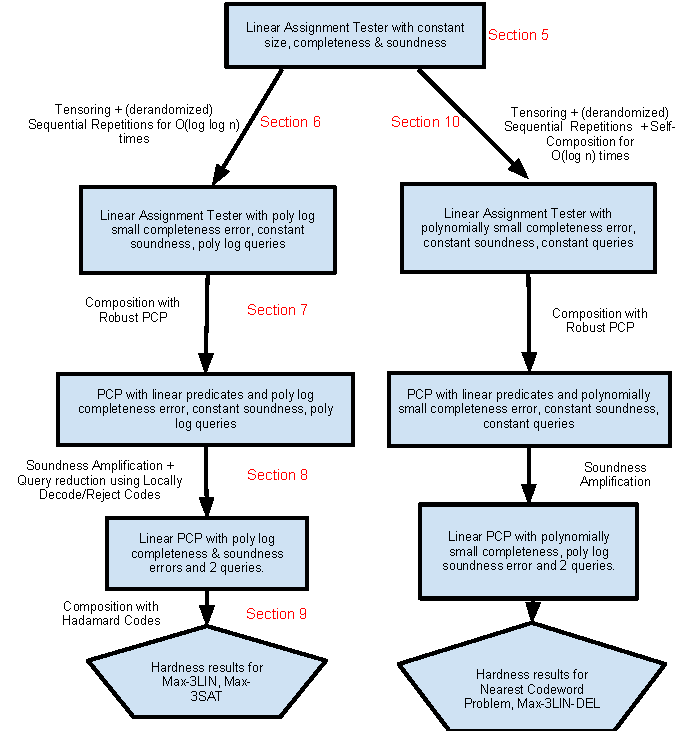
\includegraphics{Layout}
\caption{Layout of our Construction.}
\label{figure:layout}
\end{figure}

\newpage
%{\huge{Appendix}}

\section{Assignment Testers} \label{section:basic} In this section, we
construct a PCP verifier with a linear tests. In what follows, we work
with assignment testers. The notion of assignment testers was
pioneered by \cite{DR,BGHSV,S99}. They are (also) sometimes referred
to as PCP of Proximity. A related notion was recently explored as
Locally Decode and Reject Codes (LDRC) \cite{MR08} (ref. Definition
\ref{def:LDRC}) and as {\sf dPCP} by \cite{DH}.  Informally, an
assignment tester not only needs to accept a correct proof almost
always, but reject a purported proof which is far from any valid
proof. Note that this is a stronger requirement to that of a PCP where
one aspires to verify only if there is a valid proof or not. We
restrict ourselves to {\em linear} assignment testers. These are
assignment testers where the verifier's predicate is a linear function
over its variables.

\begin{definition}[Assignment Tester] \label{AT} An $(1 - \rho,
  \delta)$-Assignment Tester is a reduction whose input is a Boolean
  constraint $\psi$ over a set of Boolean variables $X$. The output of
  the reduction is a system of constraints $\Psi$ over variables $X$
  and auxiliary variables $Y$ such that for every assignment $\pi: X
  \rightarrow \{0,1\}$,
\begin{itemize}
\item {\sf Completeness:} If $\pi$ satisfies $\psi$ then there exists
  an assignment $\tilde{\pi} : Y \rightarrow \{0,1\}$ such that $\pi
  \cup \tilde{\pi}$ satisfies at least $1 - \rho$ fraction of
  the constraints in $\Psi$.
\item {\sf Soundness:} For every $\delta' < \delta$, if $\pi$ is
  $\delta'$-far from a satisfying assignment for $\psi$, then for
  every assignment $\tilde{\pi}: Y \rightarrow \{0,1\}$, at least
  $\Omega(\delta')$ fraction of the constraints in $\Psi$ reject $\pi \cup
  \tilde{\pi}$.
\end{itemize}
\end{definition}

From now on, it will be useful to use the set $\{+1 , -1\} = \{\pm
1\}$ instead of $\{0,1\}$. We use the following map $b \mapsto (-1)^b$
(that is, $0 \mapsto 1$ and $1 \mapsto -1$). Also note that this maps
the addition in $GF(2)$ into multiplication operation over
$\mathbb{R}$.


\paragraph{Standard Definitions.} We identify the {\em long code} of
${\bf x} \in \{\pm 1\}^s$ by $\LC$({\bf x}) $= \{ f({\bf x}) | f :
\{\pm 1\}^s \rightarrow \{\pm 1\} \}$. Informally, we evaluate {\bf x}
on every Boolean function on $s$ bits. Notice that every Boolean
function on $s$ bits may be represented by its truth table. In other
words, by specifying its evaluation on all the $2^s$
inputs. Alternatively, any string of length $2^s$ may be interpreted
as a Boolean function on $s$ bits. We denote $2^s$ by $n$. Since,
there are $2^{n}$ Boolean functions on $s$ bits, $\LC({\bf x})$ is a
string on length $2^{n}$. We use the letters $f, g$ to denote Boolean
functions. It is easy to check that given a table $A$, $ A \equiv
\LC({\bf x} : \{ \pm 1\}^s \rightarrow {\pm 1}$, $A(f) A(g) =
A(fg)$. That is, $A$ is closed under multiplication.

For $\alpha \subset [n]$, define
\[
          \chi_\alpha : \{\pm 1\}^n \rightarrow \{\pm 1\},  \chi_\alpha(f) \triangleq \prod_{i\in \alpha}f(i)
\]

It is easy to check that the characters $\{\chi_\alpha\}_{\alpha
  \subseteq [n]}$ form an orthonormal basis for the space of functions
$\{A : \{\pm 1\}^n \rightarrow \mathbb{R}\}$, where inner product is
defined by $\langle A, B \rangle = \mathbb{E}_f[A(f) B(f)] =
2^{-n}\sum_fA(f)B(f)$. It follows that any function $A: \{\pm 1\}^n
\rightarrow \{\pm 1\}$ can be written as $A = \sum_\alpha
\hat{A}_\alpha \cdot \chi_\alpha$, where $\hat{A}_\alpha =\langle
A,\chi_\alpha \rangle$.

\paragraph{The Long Code Test.}\label{LC} Let $A : \{ \pm 1\}^n \rightarrow \{\pm 1\}$. 
We intend to test if $A : \{\pm 1\}^n \rightarrow \{\pm 1\}$ is in
fact the legal encoding of a value $i \in [s]$. In other words, if
$A(f) = f(i)$ for all $f \in [2^n]$.

Fix a parameter $\rho \in [0,1]$. The test picks two uniformly random
vectors $f,g \in \{\pm\}^n$ and then ${h} \in \{\pm\}^n$ according to the
following distribution: for every coordinate $i \in [n]$, with
probability $1 - \rho$ we choose $h_i = 1$ and $h_i = -1$ otherwise.
It is useful to imagine ${h}$ as a noise vector. The test accepts iff
$A({f}) A({g}) = A({fgh})$.\eat{ In other words, iff $h_w = 1$, which
  happens with probability $1 - \rho$. It follows from the
  construction that the test accepts any valid long code encoding with
  probability $1 - \rho$. We now state a certain converse of that,
  which was establised by H{\aa}stad's lemma \cite{Has97}.
\begin{lemma}[H{\aa}stad's lemma \cite{Has97}]
  If the test accepts $A$ with probability $1/2 + \delta$, then
  $\sum_\alpha \hat{A}^3_\alpha \cdot (1 - 2\rho)^{|\alpha|} \ge
  2\alpha$.
\end{lemma}

\begin{lemma}[Corollary 22.25 in \cite{AB}]
  For every $\delta, \epsilon > 0$, if $A$ passes the long code test
  with probability with $1/2 + \delta$, then for $k =
  \frac{1}{2\rho}\log\frac{1}{\epsilon}$, there exists $\alpha$ with
  $|\alpha| \le k$ such that $\hat{A}_\alpha \ge 2\delta - \epsilon$.
\end{lemma}
}
\newcommand{\E}[2]{{\mathbb{E}}_{#1}\left[#2\right]}
%\newcommand{\expect}[2]{{\mathbb{E}}_{#1}\left[#2\right]}

\begin{lemma}[Tester Lemma]\label{longcode}
  For every $\delta > 0$, table $A$ which is $\delta$-far from any
  valid long code encoding is rejected with probability at least
  $\Omega(\delta)$.
\end{lemma}
\noindent {\em Proof.}  Assume that $A$ passes the test with
probability $1 - \delta$, then $\E{}{A(f)A(g)A(fgh)} = 1 -
2\cdot\delta$. Replacing $A$ by its Fourier expansion, we have

\begin{align*}
  1 - 2 \cdot \delta  &= \E{f,g,h}{\left(\sum_\alpha \hat{A}_\alpha\chi_\alpha(f) \right) \cdot \left(\sum_\beta \hat{A}_\beta\chi_\beta(g) \right) \cdot \left(\sum_\gamma \hat{A}_\gamma\chi_\gamma(fgh)\right)}\\
 &=\E{f,g,h}{\sum_{\alpha,\beta,\gamma}\hat{A}_\alpha\hat{A}_\beta\hat{A}_\gamma\chi_\alpha(f) \chi_\beta(g) \chi_\gamma(f) \chi_\gamma(g) \chi_{\gamma}(h)}\\
 &= \sum_{\alpha,\beta,\gamma}\hat{A}_\alpha \hat{A}_\beta \hat{A}_\gamma \E{f,g,h}{\chi_\alpha(f) \chi_{\beta}(g) \chi_{\gamma}(f) \chi_{\gamma}(g) \chi_{\gamma}(h)}
\end{align*}

\noindent Since the fourier basis are orthonormal, the expectation is $0$ unless $\alpha = \beta = \gamma$. Therefore,
\[
1 - 2\delta = \sum_\alpha \hat{A}_\alpha^3 \E{h}{\chi_\alpha(h)}\\
\]
\noindent Because $\E{h}{\chi_\alpha(h)} = \E{h}{\prod_{w \in
    \alpha}h_w} = (1 - 2\rho)^{|\alpha|}$, as each coordinate of $h$ is
chosen independently. Hence,
\begin{align*}
  1 - 2 \delta &= \sum_{\alpha} \hat{A}_\alpha^3 (1 - 2\rho)^{|\alpha|} \\
  &\le \sum_{\alpha} \hat{A}_\alpha^2 \cdot 1 \cdot (1 - 2\rho)^{|\alpha|} \ \ \ \ \  \ \  \because \hat{A}_\alpha \le 1\\
  &\le \sum_{|\alpha| =1} \hat{A}_\alpha^2 (1 - 2\rho) + \sum_{|\alpha| > 1} \hat{A}_\alpha^2 (1 - 2\rho)^{|\alpha|}, \ \ \  \ \hat{A}_\emptyset = 0 \ \ \mbox{due to folding}
%  &\le \sum_{|\alpha| =1} \hat{A}_\alpha^2 (1 - 2\rho) + \sum_{|\alpha| > 1} \hat{A}_\alpha^2 (1 - 2\rho)^{|\alpha|}  \\
 \end{align*}

 \noindent Since $A$ is assumed to have been folded, $\hat{A}_{\alpha}
 = 0$ if $|\alpha|$ is even. Hence, $(1 - 2\rho)^{|\alpha|} \le (1 -
 2\rho)^{3}$.  Therefore, the above expression can be written as follows.
\begin{align*}
  1 - 2\delta &\le \sum_{|\alpha| =1} \hat{A}_\alpha^2 (1 - 2\rho) + \sum_{|\alpha| > 1} \hat{A}_\alpha^2 (1 - 2\rho)^{3} \\
  & \le (1 -\Phi) (1 - 2\rho) + \Phi ( 1 - 2\rho)^{3} \ \ \ \  \ \ \
  \mbox{Let} \sum_{\alpha, |\alpha| > 1}\hat{A}^2_\alpha = \Phi\\
 1 - 2\delta &\le (1 - 2\rho) (1 - \Phi + \Phi (1 -2 \rho)^2) \\
{1 - 2\delta}/{1 - 2\rho} & \le (1  - \Phi (1 - (1 - 2\rho)^2)\\             
1 - 2(\delta - \rho) & \le 1 - \Phi (1 - (1 - 2\rho)^2)\\
\Phi & \le 2(\delta - \rho)/(4\rho - 4\rho^2)
\end{align*}
\noindent Since, $\rho$ is a fixed parameter, we have $\Phi = {\cal
  O}(\delta)$ At which point, we recall a result of Friedgut, Kalai
and Naor \cite{FKN} which (informally) states that if the fourier
coefficients are concentrated on the lowest two levels, then the
function is close to a constant function or a function that is
determined by a single coordinate.

\begin{theorem}[Theorem B.4, Page 41 in \cite{Dinur}]\label{FKN}
  There is a global constant $C'$ (independent of $n$) such that the
  following holds. Let $\Phi > 0$ and let $A : \{1, -1\}^n \rightarrow
  \{1, -1\}$ be a Boolean function for which $\sum_{\alpha, |\alpha|
    >1} |\hat{A}_\alpha|^2 < \Phi$. Then either $|\hat{A}_\emptyset|^2
  \ge 1 - C'\Phi$, or for some $i \in [n]$, $|\hat{A}_{\{i\}}|^2 = 1 -
  C'\Phi$.
\end{theorem}


\noindent Therefore, by folding, there must be some $i$ such that $\psi(i) = -1$
and $\chi_{i}$ is ${\cal O}(\Phi)$. Theorem \ref{FKN} also allows $-
\chi_i$ to be ${\cal O}(\Phi)$-close to $A$, but this causes the test
to fail with probability close to $1/4$, which is certainly
$\Omega(\delta)$. Hence, we showed that unless $A$ is $\delta$-close
to some $\chi_{i}$ for the value of $i$ that satisfies $\psi$, at
least $\Omega(\delta)$ of the tests must be
rejected. \qed \\






\eat{That is,
\begin{align*}
  \	   \Pr \left [A\ \mbox{passes}\ \right]  &\ge 1 - \delta \\
  & \implies   \hat{A}_k \ge 2 \cdot (1/2 -\delta ) - \epsilon \\
  &\implies  \exists \alpha \subset [n],  |\alpha|  \le k \  \mbox{s.t.}\  \chi_\alpha \  \mbox{is}\  \Omega(\delta')\mbox{-far}\ \mbox{from}\  A \\
 \end{align*}
 Note that $\chi_\alpha$ can be expressed as $\prod_{i \in \alpha}
 \chi_i$ and $|\alpha|$ is a constant.  Thus, any of the $\chi_i$'s
 agrees with $\chi_\alpha$ on at least $2^{-|\alpha|}$ fraction of the
 domain. Putting this in the context of agreement between $A$ and
 $\chi_i$: $\chi_i$ disagrees with $A$ on at least $1/2^{|\alpha|}
 \cdot \delta'$ fraction, which is essentially
 $\Omega(\delta)$. \qed\\}

  
 
\noindent We are now ready to present the assignment tester needed for
our construction. Let $\psi$ be a Boolean constraint over Boolean
variables $x_1, x_2 \ldots x_s$. We describe an algorithm whose input
is $\psi$ and whose output will be a system of linear equations
satisfying the requirements of Definition \ref{AT}. The tester seeks
as input a satisfying assignment $\sigma$ to $\psi$ and the
$\LC(\sigma)$, the long code of $\sigma$. One may imagine $\LC(\sigma)$
as the set of auxilary variables used by the tester. \\

 
\noindent Also, as done in \cite{BGS}, we fold the long code tables
over true and the respective constraint $\psi$. This means that
whenever the test needs to read $A[f]$, it reads $A[\psi \wedge f]$
instead. In addition, we fold over true which means for every pair $f$
and $-f$, we let $A$ specify only one and access the other via the
identity $A[f] = - A[f]$. In short, we assume that $A[f] = A[f \wedge
\psi]$ and $A[f] =- A[-f]$ for all $f$. It is well known that after
folding $\hat{A}_\alpha = 0$ whenever $|\alpha|$ is even or there
exists an $i$ in $\alpha$ for which $\psi(i) = 1$ (recall that $1$
corresponds to false). An interested reader may refer to Lemma 22.27
on page 482 of \cite{AB}. We elaborate on the latter. Set $f' = f +
e_i$, where $i$ is an index such that $\psi(i) = 1$. Now,
$\chi_\alpha(f) = - \chi_\alpha(f')$ but $A[f] = A[f']$. We now
describe the two kinds of constraints we place over these
variables. Say, the tester gets two tables $\sigma$ and $A$ as input.

\begin{enumerate}
\item {\sf Long Code Constraints:} The first set of constraints aims
  at testing if $A$ is indeed a valid long code encoding. It includes
  $3$ variable constraints derived from the {\em long code} test
  specified earlier. Specifically, we shall fix $\rho$ to be a
  non-zero constant and have one constraint per each coin toss of the
  long code test.

\item {\sf Consistency Constraints:} The second set of constraints
  include the following: For each choice of $i \in [s]$ and $f$
  place a constraint that is satisfied iff $\sigma(x_i) = A(f) \oplus
  A(f \oplus e_i)$\footnote{$e_i$ is the vector of dimension $2^s$
    with a $-1$ in $i$-th index and $1$ elsewhere.}. For the ease of
  argument, assume that are an equal number of constraints of each
  type\footnote{This can be easily achieved by placing multiple copies
    of the constraint of each type with appropiate multiplicity.}.
\end{enumerate}

\begin{lemma}[Assignment Tester] \label{Tester} For any $\rho, \delta
  > 0$, the constraint system constructed above is a $(1- \rho,
  \delta)$-assignment tester for any Boolean function $\psi : [s]
  \rightarrow \{0,1\}$. Moreover, the assignment tester is a linear
  function on its input.
\end{lemma}
\noindent {\em Proof.} Linearity of the constraints follows from
construction. We now analyze the parameters of the tester below
parameter by parameter.

\begin{itemize}
\item {\em Completeness:} We set the probability of generating the
  noise vector {$h$} in the long code test to $1 - \rho$. Now, for any
  good assignment that satisfies the constraint $\psi$, the second set
  of constraints are always satisfied. The only case where we reject a
  good proof is during the long code test and this happens with
  probability at most $\rho$.

\item {\em Soundness:} Say, the tester gets $\sigma$ and $\pi$ as
  input and $\sigma$ is $\delta$-far from a satisfying assignment of
  $\psi$, we shall show that the assignment tester rejects with
  probability at least $\Omega(\delta)$. {\em w.l.o.g}, we consider
  the following cases. (1) $\pi$ is $\delta$-far from any long code
  encoding. (2) $\pi$ is not $\delta$-far from a valid long code
  encoding. \\

  \noindent In the former, it follows from Lemma \ref{longcode} that
  if $\pi$ is $\delta$-far from a valid long code table is rejected
  with probability greater than $\Omega(\delta)$ and by our
  construction these constraints constitute at least
  $\Omega(\delta)$-fraction of the total constraints. Thus, we reject
  any $\pi$ that is $\delta$-far from a valid long code encoding with
  probability at least $\Omega(\delta)$.


  In the latter, since $\pi$ was folded across $\psi$, we may assume
  that $\pi$ encodes a satisfying assignment to $\psi$. Say $\pi$
  encoded a satisfying assignment ${\sigma'}$. Since, $\sigma$ is
  $\delta$-far from a satisfying assignment, it must be that $\sigma$
  is $\delta$-far from ${\sigma'}$. Hence, $Pr_i[\sigma(x_i) \ne
  \sigma'(x_i)] \ge \delta$. Since, $\pi$ is not $\delta$-far from a
  valid long code encoding, we also have that
\begin{align*}
  \Pr_{f \in [n]} \left[ \pi(f) \oplus \pi(f +e_i) = f(\sigma') \oplus (f \oplus e_i)(\sigma') \right] & \ge \Pr [\pi(f) = f(\sigma') \ \ \mbox{and} \ \ \pi(f \oplus e_i) = (f \oplus e_i)(\sigma') ] \\
 &\ge 1 - 2\delta
\end{align*}
This fails whenever $\sigma(x_i) \ne \sigma'(x_i)$, then $f(\sigma')
\oplus (f \oplus e_i)(\sigma') = \sigma'(x_i) \ne \sigma(x_i)$. And
this is at least $\delta (1 - 2\delta) = \Omega(\delta)$. \\

\noindent Hence, in either case we would have rejected $\sigma \circ
\pi$ with probability at least $\Omega(\delta)$. Because, there are an
equal number of constraints of each type, we reject an invalid proof
$\pi$ with probability at least $\Omega(\delta)$.

\item {\em Query Size:} The tester picks at random a long code
  constraint or a consistency constraint and verifies it. In either
  case, it makes $3$ queries.

\item {\em Randomness:} The tester uses $2 \cdot s$ bits of
  randomness. \qed
\end{itemize}



We denote the {\sf size} of a linear tester by the $n$ and it refers
to the quantity $q \cdot m$, where $q$ is the number of queries made
by the tester and $m$ is the total number of equations in the
tester. Linear assignment testers cannot have perfect completeness.
For otherwise, one may use guassian elimination to figure out the if
there is an assignment that satisfies all the linear constraints and
reject if there isn't one. Hence, any linear tester is forced to have
a non-zero completeness error. Also, the soundness is always less than
$1/2$ as a random assignment satisfies at least $1/2$ of the equations
in $\eL$ in an expected sense (follows from the fact that the
equations are over ${GF}(2)$). As highlighted earlier, having low
completeness error becomes handy in several scenarios. We now
highlight on how we intend to use the tools we developed in the
previous section to achieve completeness amplification.


\section{Completeness Amplification}  \label{section:complete}

In this section, we employ tensoring to amplify the completeness of
the assignment tester we have built in Section \ref{section:basic}.
In what follows, we start with notations and a few observations that
will be useful to us in amplifying the completeness of the assignment
tester.\eat{ Let $\eL \equiv {\bf Ax} + {\bf y} = {\bf 0}$ denote the
  linear assignment tester given to us by Lemma \ref{Tester}. We now
  show that the d($\A$), d($\A$) $\equiv \min_{{\bf x} \ne {\bf 0}}
  {\bf Ax}$, is non-zero.

\begin{proposition}\label{longcodeisbest}
  Let $\eL \equiv {\bf Ax} + {\bf y} = {\bf 0}$ be the assignment
  tester obtained via Lemma \ref{Tester}. Then, for every ${\bf x_1}$
  and ${\bf x_2}$, ${\bf x_1} \ne {\bf x_2}$, the Hamming weight of
  ${\bf A} \cdot ({\bf x_1} + {\bf x_2})$ is a non-zero quantity. In
  other words, d($\A$) $> 0$.
\end{proposition}
\noindent {\em Proof.} To establish this, we consider the long code
constraints. Observe that the constants in the long code constraints
arise from the noise vector {h}. Thus, modulo the noise vector the
long code constraints are over auxilary variables $\pi$ of the tester
and are the following: $\Pi$ = $\pi(i) + \pi(j) + \pi(i + j) \ \forall
\ i,j \in |\pi|$. Now, since ${\bf x_1} \ne {\bf x_2}$, they either
differ on exactly $0 < k \le |\pi|$ coordinates. ${\bf x_1}$ and ${\bf
  x_2}$ evaluate different on every equation in $\Pi$. In the latter,
say they disagree on $\pi({\bf 0})$, then they evaluate differently on
$\pi(\alpha) + \pi({\bf 0}) + \pi(\alpha + {\bf 0})$. If however they
agree on $\pi({\bf 0})$, then either they disagree only one coordinate
$\beta$ or on more than one coordinates. In the former, ${\bf x_1}$
and ${\bf x_2}$ disagree on $\pi(\beta) + \pi(\alpha) + \pi(\alpha +
\beta)$. \qed }

\begin{definition} Let ${\cal T}$ denote the assignment tester
  obtained via Lemma \ref{Tester} and $\psi : [s] \rightarrow \{0,1\}$
  denote the Boolean predicate being tested. For any proof $\Psi$
  provided to ${\cal T}$, we denote by $\Pi_\psi$ the assignment
  induced by $\Pi$ on the variables of $\psi$. Also, we denote by
  $\psi(\Pi_\psi)$ the evaluation of $\psi$ on $\Pi_\psi$. 
\end{definition}

\begin{observation} \label{invariant} For any given proof $\Pi$ to
  assignment tester ${\cal T}$ to verify the satisfiability of $\psi$,
  $\Pi^{\otimes 2}_\psi$ is exactly same as $\Pi_\psi$. More
  importantly, the distance of $\Pi_\psi$ to a satisfying assignment
  of $\psi$ remains uneffected by tensoring. Moreover, the converse
  also holds. That is, for any purported proof $\Pi$ to a tensored
  system and its the diagonal entries, denoted by $\pi$, $\pi_\psi$ is
  same as $\Pi_\psi$.
\end{observation}
\noindent {\em Proof Sketch.} Since, we are working with $GF(2)$, it
follows from the defintion of tensoring that the diagonal entries
$\{x_{ii}\}$ of $\Pi^{\otimes 2}$ preserve $\Pi$. Thus, $\Pi_\psi$ and
$\Pi^{\otimes 2}_\psi$ are exaclty the same. The converse follows from
the fact that we extract (decode) the assignment $\pi$ from $\Pi$ by
reading
its diagonal entries. \qed\\


In fact, both directions of the aforementioned observation can be
extended to any $\Pi^{\otimes k}$, $\Pi^{\otimes j}, \ 0 < j \le
k$. We are now ready to amplify the completeness of the basic
assignment tester we have constructed in Lemma \ref{Tester}.

\begin{lemma}[Tensored Assignment Tester] \label{tensortester} For
  every $\rho, \delta > 0$, there is a $(1 - \rho^2,
  \delta^2)$-assignment tester for any Boolean function $\psi : [s]
  \rightarrow \{0,1\}$. Moreover, the predicate of the assignment
  tester is linear.
\end{lemma}
\noindent {\em Proof.} We invoke Lemma \ref{Tester} to construct an
$(1 - \rho, \delta)$-assginment tester ${\cal T}$. The tests performed
by our new $(1 - \rho^2, \delta^2)$-assginment tester, denoted by
${\cal T}^{\otimes 2}$, will be tensored tests of ${\cal T}$. In other
words, if the tests of ${\cal T}$ are $\eL$, then the tests of ${\cal
  T}^{\otimes 2}$ are linear equations in $\eL^{\otimes 2}$
(ref. Definition \ref{Tensoring}). Let $\Pi$ denote proof required by
${\cal T}$. The proof to $(1 - \rho^2, \delta^2)$-assginment tester
${\cal T}^{\otimes 2}$ will be ${\Pi}^{\otimes 2}$. Thus, the new
proof format will be $(\sigma \circ \pi)^{\otimes 2}$ and the
variables of $\psi$ will be $\{ \sigma_{ii}\}$ and the rest will be
auxilary variables of ${\cal T}^{\otimes 2}$. We shall now analyze the
parameters of ${\cal T}^{\otimes 2}$.
\begin{itemize}
\item {\em Completeness:} In the good case, if there is a proof
  $\sigma \circ \pi$ which ${\cal T}$ accepts with probability at
  least $1 - \rho$. We invoke Proposition \ref{basic} to conclude that
  the probability that ${\cal T}^{\otimes 2}$ accepts $\left(\sigma
    \circ \pi\right)^{\otimes 2}$ is at least $1 -$UNSAT($\eL, \sigma
  \circ \pi$)$^2$, which is $1 - \rho^2$.

\item {\em Soundness:} We shall establish that for any purported proof
  $\Pi$ to ${\cal T}^{\otimes 2}$, if $\Pi_\psi$ is $\delta^2$-far
  from a satisfying assignment to $\psi$, then ${\cal T}^{\otimes 2}$
  rejects with probability at least $\Omega(\delta^2)$.  In order to
  establish this, we deal with the contrapositive of the claim.  Say,
  if $\Pi$ is accepted with probabilty $1 - \delta^2$, we shall show
  that $\Pi_\psi$ is not $\Omega(\delta^2)$-far to a satisfying
  assignment of $\psi$.

  Say, $\Pi$ is accepted with probability at least $1 - \delta'$, we
  can use Lemma \ref{converse} to infer that the diagonal vector of
  ${\Pi}$ gives us a proof which ${\cal T}$ accepts with probability
  at least $\alpha = 1 - \lfloor \frac{\delta'}{\delta}\rfloor$, where
  $\delta' < 1/16$. For the parameters that we have choosen, if
  $\delta' = \Theta(\delta^2)$ then $\alpha \simeq 1 -
  \Omega(\delta)$. In other words, if $\Pi$ has an acceptance
  probability of $1 - \delta^2$, then we can decode a proof $\pi$,
  which ${\cal T}$ would accept with probability $1 -
  \Theta(\delta)$. And from Lemma \ref{Tester}, we know that if ${\cal
    T}$ accepts $\pi$ with probabilty $1 - \Theta(\delta)$, then
  $\pi_\psi$ isn't $\Omega(\delta)$-far from a satisfying assignment
  of $\psi$.

  But, from Observation \ref{invariant} we can infer that $\Pi_\psi$
  is exactly same as $\pi_\psi$. Thus, if $\pi_\psi$ is not
  $\delta$-far from a satisfying assignment of $\psi$, so is
  $\Pi_\psi$. Also, by hypothesis, ${\cal T}^{\otimes 2}$ accepts
  $\Pi$ with probability $1 - \Theta(\delta^2)$. Hence, we can
  conclude that for every $\Pi$, if $\Pi$ is accepted with probability
  at least $1 - \delta^2$, then $\Pi_\psi$ is not $\Omega(\delta)$-far
  from a satisfying assignment. Since $\delta^2 < \delta$, it follows
  that if $\Pi_\psi$ is $\delta$-far from a string, it is
  $\delta^2$-far. Therefore, the soundness of ${\cal T}^{\otimes 2}$
  holds.
\item {\em Query size:} ${\cal T}^{\otimes 2}$ needs to make as many
  queries as the number of variables in an equation of $\eL^{\otimes
    2}$. And this happens to be $\q^2$, where $\q$ is query size of ${\cal T}$.

\item {\em Randomness:} The randomness used by ${\cal T}^{\otimes 2}$
  is $\log \eL^{\otimes 2}$, which is $2 \cdot \log \eL$. In general,
  if we blow up the randomness by a factor of $k$ whenever we tensor
  an assignment tester $k$ times.\qed
\end{itemize}


\noindent Notice that the above transformation preserves the linearity
of the tester. The downside of tensoring is that while it enhances the
completeness, it also destroys the soundness. Ideally, we would like
to improve the acceptance probability of the verifier in the good case
and leave the acceptance probability in the bad case unperturbed. Thus
to improve the soundness of the tester after the tensoring operation,
we invariably resort to soundness amplification.

\subsection{Soundness Amplification Perserving Linearity}
Soundness amplification of a PCP can achieved via some kind of
repetition, either sequentially or in parallel. Repetition of a PCP
involves repeating the tests with independent randomness. For
instance, performing sequential repetition once would involve 
repeating the assignment tester on two independently drawn tests 
and accepting them iff both are satisfied. This transforms an $(1 - \rho,
\delta)$-assignment tester into an $(1 - 2 \cdot \rho ,2 \cdot
\delta)$-assignment tester. In general, performing sequential
repetition for $\vartheta$ times on $(1 - \rho , \delta)$-tester leaves us
with a $(1 - \vartheta \cdot \rho, \vartheta \cdot
\delta)$-tester. However, this operation does not preserve
linearity. 


Thus, we resort to a different kind of soundness amplification. We
pick ${\cal O}(1)$ tests of the assignment tester and then, adds all
possible linear combinations of these tests to the create a new
assignment tester. The idea is that even if one the ${\cal O}(1)$
 equations are not satisfied by some assignment, half of the linear
combinations of these equations will also not be satisfied by the
assignment. This also happens to preserve the linearity. However, to
keep the size of the output assignment tester instance small, we
pseudo-randomly generate only ${\cal O}(n)$ of the $n^{{\cal O}(1)}$
possible ways to pick ${\cal O}(1)$ tests from $n$ tests.

Given a $(1 - \rho^2, \delta^2)$-assignment tester as an input, we
wish to produce an $(1 - \rho^2, \delta)$-assignment tester as the
output. We achieve this via randoms walks on expanders. We aim to
achieve the following by taking a random walk on a expander: the
probablilty of visiting a subset containing a certain fraction
($\delta^2$ in our case) of the vertices is at least $2 \cdot
\delta$. And since, at least half of the linear combinations having an
unsatisfied equation also remain unsatisfied, we would end up with our
cherished objective of amplifying the soundness to $\delta$.

We begin by defining a {\em walk of length l} in a graph $G = (V,E)$
is a sequence $v_0, \ldots v_l$ of vertices of $G$, where for $1 \le i
\le l$, $v_{i-1}v_i$ is an edge in $G$. By a simple calculation, the
total number of walks of length $l$ in any $d$-regular graph is
exactly $|V|\cdot d^l$. Suppose there is a subset $C$ of $V$, we wish
to bound the number of walks that do not contain a vertex from $C$. If
$G$ happens to be disconnected, it may happen that a constant fraction
of them avoid $C$. However, Ajtai, Koml\'{o}s and Szemr\'{e}di
\cite{AKS87} showed that if all the eigenvalues of $G$, with the
exception of the largest, are small, then there are far fewer of walks
avoiding $C$. We now state their result.

\begin{theorem} \label{walks} Let $G = (V,E)$ be a $d$-regular graph
  on $n$ vertices, and suppose that each of its eigenvalues but the
  first one is at most $\lambda$. Let $C$ be a set of $cn$ vertices of
  $G$. Then, for every $l$, the number of walks of length $l$ in $G$
  that avoid $C$ does not exceed $(1 - c)\cdot n \cdot ((1 - c) \cdot
  d + c \cdot \lambda)^l$.
\end{theorem}

Now, a {\em randomly chosen walk} of length $l$ in $G$ chosen
according to a uniform distribution among all walks of that length.
If $G$ is regular, then such a walk can be chosen by choosing its
starting point $v_0$ uniformly at random and then picking the next
vertex of the walk among the $d$ neighbours of $v_0$ uniformly at
random. We are now ready to state a Corollary of Lemma \ref{walks}
which will be very useful for us.

\begin{corollary}\label{randomwalks}
  Let $G = (V,E), d, n, \lambda, C$ and $c$ be as in Theorem
  \ref{walks} and suppose 
\[
(1 - c)\cdot d + c \cdot \lambda \ \le \ \frac{d}{\sqrt{2}}
\]
Then, for every $l$, the probability that a randomly chosen walk of
length $l$ in $G$ avoids $C$ is at most $2^{{-l}/{2}}$.
\end{corollary}

\eat{In this work, we make use of a samplers based approach. Samplers
  are pseudo-random objects that are extremely useful in simulating a
  random walk or drawing random samples. In what follows, we denote
  the neighbours of a vertex $u$ in a graph by $\Gamma(u)$.

\begin{definition}[Samplers]
  A bipartite graph $H = (A,B,E)$ is said to be an $(\epsilon,
  \gamma)$-sampler if for every subset $S \subseteq A$,
\[
  \Pr_{b \in B}\left[ \frac{|\Gamma(b) \cap S|}{|\Gamma(b)|} > \frac{|S|}{|A|} + \epsilon \right] \le \gamma
\]
\end{definition}

In other words, neighbourhoods of most vertices $b$ behave like a
random sample of $A$, in the sense that that their density within any
fixed $S$ is close to what is expected.  The following article
\cite{Sample} by Oded Goldreich is an excellent exposition on
samplers, their constructions and applications.

\begin{theorem}\cite{Sample}\label{sample} There exists a polynomial 
  time algorithm that, given an integer $n$ and a parameter $\epsilon
  > 0$, outputs an $(\epsilon, \gamma)$-sampler with $|A| = |B| = n$
  and the right degree $4/\epsilon^4$. Moreover, the randomness used
  by the algorithm is bounded by $\log n + {\cal O}(\log 1/\epsilon )
  + {\cal O}(\log  1/\gamma)$.
\end{theorem}
}
\begin{lemma}[Soundness Amplification] \label{boosting} There is
  universal constant $\vartheta$, such that every $(1 - \rho^2,
  \delta^2)$-assignment tester for a Boolean predicate $\psi$ over
  variable set $\sigma$ can be amplified to a $(1 - \vartheta \cdot
  \rho^2, {\delta})$-assginment tester. Moreover, the new tester still
  has a linear predicate.
\end{lemma}
\noindent {\em Proof.} Let us denote the $( 1 - \vartheta \cdot
\rho^2), \delta^2)$-assignment tester by $V$ and the tests performed
by $V$ with $\eL$. Our approach will be to design a new assignment
tester $V'$ whose tests are the sum of $\vartheta$ tests of the old
verifier $V$. We construct a graph $G$ in which the vertices are the
tests of $V$. Let $\phi_i$ denote the equation (constraint) at vertex
$v_i$. We then pick a (test) vertex $v_1$ uniformly at random. We then
take a random walk of length $\vartheta$ starting at $v_1$. The new
tests will be the sum of tests at each of these vertices. Thus, $\eL'
= \{ \phi_1 \oplus \phi_2 \ldots \oplus \phi_\vartheta : \phi_i \in
\eL\}$. We fix $\vartheta$ to be the length of random that one must
take on an expander so that the probability we hit a $\delta^2$
fraction of the tests is at least $2 \cdot \delta$. It follows from
Corollary \ref{randomwalks} that for an appropiate choice of expander
and some constant $\vartheta$ less than $5$ it holds that the
probability we hit a $\delta^2$ fraction of the vertices is at least
$2 \cdot \delta$. Note that even though the tests of $V'$ are
different from $V$, both of them expect the same proof as in Lemma
\ref{Tester}. We now establish that $V'$ is in fact a $(1 - \vartheta
\cdot \rho^2, {\delta})$-assignment tester.
\begin{itemize}
\item {\em Completeness:} In the good case, $V$ reject a valid proof
  with probability at least $\rho^2$. Now by basic probability, the
  probability that $V'$ accepts a valid proof it is at most $(1 - \rho^2)^\vartheta$, 
  which is bounded from below by $(1 - \vartheta \cdot \rho^2)$.
 
\item {\em Soundness:} Say, we are given an assignment tester $V$ that
  rejects any proof $\Pi$ if $\Pi_\psi$ (projection of $\Pi$
  on the variable set $\sigma$) is $\delta$-far from a satisfying
  assignment of $\psi$, it is rejected with probability at least
  $\Omega(\delta^2)$. The claim we make is that the assignment tester
  $V'$ will get reject any $\Pi$ such that $\Pi_\psi$ is $\delta$-far
  from a satisfying assignment to $\psi$ with probabilty at least
  $\Omega({\delta})$. Consider the scenario that $V$ rejects a proof
  with probability $\delta^2$. It follows from our parameters 
  that probability the random walk hits the bad set is
  at least $2 \cdot \delta$ and at least half of these tests fail over
  the choice of our random walk. Thus, the probability the we accept
  an invalid proof is bounded from above by $1 - \delta$. In other
  words, if $V$ rejected an invalid proof with probability at least
  $\delta^2$, the new tester would reject it with probability at least
  $\delta$. The distance parameter of $\Pi_\psi$ is uneffected by this
  operation and hence, we inherit from Lemma \ref{Tester} and 
  \ref{tensortester} that if $\Pi_\psi$ was $\delta$-far from
  a satisfying assignment, it continues to be so.
 
\item {\em Query size:} The arity of the equations in $\eL'$ is $\vartheta
  \cdot q$, where $q$ is the arity of $V$.

\item {\em Randomness:} Since, we are choosing a test of $V$ uniformly
  at random and then taking a random walk of length $\vartheta$ on an
  expander $G$ with a constant degree, we would be needing $r_V +
  {\cal O}(\vartheta)$, where $r_V$ is the randomness used by $V$.\qed
\end{itemize}


\eat{
  \begin{lemma}[Derandomization Lemma] \label{derandomize} For every
    $\rho > 0, \delta < 1/4$, $\vartheta < \min(1/\rho,1/\delta)$ and
    $\vartheta$ sequential repetitons of every ($\rho,
    \delta$)-assignment tester can be achieved using only $r_v + {\cal
      O}(\vartheta)$ random bits.
\end{lemma}
\noindent{\em Proof.} Follows by invoking Theorem \ref{sample} to
construct a $(\epsilon, \gamma)$-sampler and use it instead of
sampling $\vartheta$ tests of verifier at random. Specifically, set $n
= 2^{r_v}$, $\gamma = 1- \vartheta \cdot \delta$, $\epsilon$ will be
fixed latter.  We now establish that this process actually simulates
sequential repetition in a randomness efficient way. During sequential
repetition, we wish to test independent samples of the verifier's
test. Consider the soundness case, here we would like to sample one of
the constraints that fail the verifier's test. Say, a set $S$ of the
tests fail. So, we would like to hit one of these tests. In a
sequential repetition, the probability that we hit this set is
$\vartheta \cdot \frac{|S|}{|A|}$.

We aim to achieve the aforementioned claims via a sampler. For a
sampler to have failed us, it must be that the vertex $b$ on the right
must have had all its neighbours in the complement (denote this set by
$\overline{S}$) of $S$ that we wanted to hit. And, the probability
that this would happen is
\begin{align*}
  \Pr_{b \in B}\left[ \frac{|\Gamma(b) \cap \overline{S}|}{|\Gamma(b)|} = 1 \right] 
  = \Pr_{b \in B}\left[ \frac{|\Gamma(b) \cap \overline{S}|}{|\Gamma(b)|} = 1 - \frac{|S|}{|A|} + \frac{|S|}{|A|} \right] 
  =  \Pr_{b \in B}\left[ \frac{|\Gamma(b) \cap \overline{S}|}{|\Gamma(b)|} =  \frac{|\overline{S}|}{|A|} +  \frac{|S|}{|A|} \right] 
%  =& \Pr_{b \in B}\left[ \frac{|\Gamma(b) \cap \overline{S}|}{|\Gamma(b)|} =  \frac{|\overline{S}|}{|A|} +  \frac{|S|}{|A|} \right] \\
  \end{align*}
We invoke Theorem \ref{sample} for $\epsilon \in (0, \frac{|S|}{|A|}]$.  
\begin{align*}
  \Pr_{b \in B}\left[ \frac{|\Gamma(b) \cap
      \overline{S}|}{|\Gamma(b)|} > \frac{|\overline{S}|}{|A|} +
    \epsilon \right] \le 1 - \vartheta \cdot \delta \implies \Pr_{b \in
    B}\left[ \frac{|\Gamma(b) \cap {S}|}{|\Gamma(b)|} > \epsilon
  \right] >  \vartheta \cdot \delta
\end{align*}

Hence, the completeness and soundness of this new assignment tester is
$\vartheta \cdot \rho$ and ${\vartheta} \cdot \delta$
respectively. This is essentially what we achieve with $\vartheta$
sequential repetitions as in Lemma \ref{boosting} but with a larger
query complexity $1/\epsilon^4$. If $\epsilon = \Theta(1/\vartheta)$,
then the query complexity happens to be ${\cal O}(\vartheta^4)$. The
bounds on randomness follows from Theorem \ref{sample}.
\qed\\
}
\begin{corollary}[Tensoring + Repetition]\label{iterate}
  For every $\rho > 0$ and $\delta < 1/4$, there is an absolute
  constant $\vartheta$, such that given an $(1 - \rho,
  \delta)$-assignment tester that uses $r_v$ random bits to make $\q$
  queries, one can construct an $(1 - {\cal O}\left(\rho^2\right) ,
  {\delta})$-assignment tester. The new assginment tester uses $2
  \cdot r_v + {\cal O}(\vartheta)$ random bits and makes ${\cal
    O}(\vartheta \cdot \q^2)$ queries. Moreover, our latest
  construction has a linear predicate.
\end{corollary}
\noindent {\em Proof.} We start with the assignment tester ${\cal T}$
given by Lemma \ref{Tester} that seeks a proof $\Pi = \sigma \circ
\pi$, where $\sigma$ are the variables of the Boolean predicate being
verified and $\pi$ is the auxilary variables introduced by the
assignment tester. Our new assignment tester ${\cal T}'$ is obtained
by invoking Lemma \ref{tensortester} and then followed by Lemma
\ref{boosting} on ${\cal T}$ with parameters $\delta = 16/100$,
$\vartheta = 5$ and $\rho = 1/\left(2 \cdot \vartheta\right)$ . The
proof required by ${\cal T}'$ will be $\Pi^{\otimes 2}$. We now argue
the completeness and soundness of the newly constructed assignment
tester.
\begin{itemize}
\item {\em Completeness:} In the good case, if we have a proof that
  the input assignment tester $T$ accepts with probability $1 - \rho$,
  we can use Proposition \ref{basic} to claim that after invoking
  Lemma \ref{tensortester} on $T$, we have a completeness of $1-
  \rho^2$. Now, after the application of Lemma \ref{boosting} it
  follows from our parameters that the completeness of $1 - {\cal
    O}(\rho^2)$.
\item {\em Soundness:} Say, the newly constructed assignment tester is
  given a purported proof $\Pi$ such that $\Pi_\psi$ (denotes the
  assignment induced on $\sigma$ by $\Pi$) is $\delta$-far from a
  satisfying assignment to $\psi$, we will need to establish that it
  is rejected with probability at least $\Omega(\delta)$. One
  important inference from Observation \ref{invariant} is that the
  neither tensoring nor soundness amplification change the assignment
  to $\sigma$ and hence, its distance to a satisfying assignment of
  $\psi$. Hence, if the input assignment tester has the soundness for
  $\delta < 1/4$, we can invoke the soundness arguments of Lemma
  \ref{tensortester} and \ref{boosting} to infer that soundness
  condition remains intact for $\delta < 1/4$. \qed
\end{itemize} 


\begin{lemma}[Completness Amplification Lemma]\label{Camplify}
  For every $\rho > 0$ and $\delta < 1/4$, given a $(1 - \rho,
  \delta)$-assignment tester with query complexity $\q = {\cal O}(1)$
  and size $2^{r_v}$, one can construct a $(1 - {\cal
    O}(\rho^k),\delta')$-assignment tester with query complexity $\q$,
  $\q = 1/\rho^{k'}$, in time polynomial in $2^{ k \cdot {\cal
      O}(r_v)}$. Also, the resulting assignment tester has a linear
  predicate.
\end{lemma}
\noindent{\em Proof.} Say we have a (1 - $\rho, \delta$)-assignment tester
that verifies a Boolean predicate $\psi$ using a proof over variables
of $\psi$ (call them $\sigma$) and auxilary variables $\pi$. The idea is to
let the tests of the $(1 - {\cal O}(\rho^k),\delta)$-assignment 
tester be the tests of lemma \ref{iterate} tensored with itself $k$ times. 
Our $(1 - {\cal O}(\rho^k),\delta)$-assignment 
tester uses the proof ($\sigma \circ \pi$)$^{\otimes k}$.

However, we would like to iteratively apply the output of Lemma
\ref{iterate} upon on itself. This makes it easier to apply the tools
that we have build thus far. The first observation we make is that the
after a $(1 - \rho, \delta)$-tester, of size $n$, under goes $r$
iterations of the tensoring followed by $\sigma$ rounds of sequential
repetition, the size of the resulting tester is
$n^{2^{2^{r-1}}}$. This can be verified once we observe that we are
squaring the size of the input instance in every iteration. By
invoking Corollary \ref{iterate}, we infer that the completeness error
is also squared in each iteration. Hence after $r$ iterations, the new
error parameter is $\rho^{2^{2^{r-1}}}$. However, the soundness of the
tester remains uneffected due to the amplification given by Lemma
\ref{boosting}. With this background, the Lemma follows by setting $ r
= \log \log k$. Notice that the proof required by this recursive
construction is same as that of the iterative assignment tester
constructed in previous paragraph.  The new proof will be $(\sigma
\circ \pi)^{\otimes k}$. Also, note that while the auxilary variables
blow up in every step, the variables of the Boolean predicate that we
are checking remain the same. The parameters are summarized in Table
\ref{roundup}.

\begin{table}
%\begin{table}
\centering
\begin{tabular}{|l|c|c|c|}
\hline
%\ & & \\
{\em Parameters}  &{ Tensoring} & {\parbox{0.9in}{Soundness\\ Amplification}} & \parbox{0.7in}{After $k$\\ Iterations}\\
	\hline
%\ &  & \\ 
        \hline
        {\tt Completeness} & $1 - \rho^2$ & 1 - ${\cal O}\left(\rho^2\right)$  & 1 - ${\cal O}(\rho^{k + 1})$ \\  
        {\tt Soundness} &   $\delta^2$ & $\delta$&  $\delta$ \\
        {\tt Queries} &   $q^2$ & $\vartheta\cdot q^2$ & $\vartheta^{\sqrt{k}+1} \cdot  q^{k} $ \\
        {\tt Alphabet}&    $\{0,1\}$ & $\{0,1\}$ & $\{0,1\}$ \\
        \hline
\end{tabular} %\caption{Parameters after one iteration} \label{1round}
  \caption{Parameters of a ($\rho, \delta$)-assignment tester after various operations.} \label{roundup}
\end{table}


\begin{itemize}
\item {\em Completeness:} It is by far the easier case to argue. Say,
  a $(1 - \rho, \delta)$-assignment tester is given to us that enables
  us to verify a Boolean predicate using a proof $\Pi$. Then by
  Corollary \ref{iterate}, we have a new assignment tester which has
  the square of the completeness error after a single iteration. It
  follows that after $\log \log k$ iterations, we end up with a
  completeness error of ${\rho^k}$.

\item {\em Soundness:} Say that the $(1 - {\cal
    O}(\rho^k),\delta)$-assignment tester is given access to a
  purported proof $\Pi$, we need to show that the if the proof
  $\Pi_{\psi}$ (denotes the assignment induced by $\Pi$ on the
  variables of $\psi$) is $\delta$-far to a satisfying proof of the
  Boolean predicate, the tester rejects with probability at least
  $\Omega(\delta)$. We show this property holds after each iteration
  and hence, the newly constructed assignment tester via this process
  always has the soundness condition.

  The approach is simple. We give a proof by induction on the number
  of iterations. The assignment tester produced after the first
  iterate is sound by Corollary \ref{iterate}. Assume that the
  assignment tester produced after $i$-th iterations is sound. We now
  show that the assignment tester produced after ($i+1$)-th iteration
  is also sound. By assumption, the assignment tester at the $i$-th
  level has the soundness property, it now follows from Corollary
  \ref{iterate} that the soundness holds even after $(i+1)$-th
  iteration.

\item {\em Queries:} We again invoke Corollary \ref{iterate} to
  conclude that the number of queries are first squared and then,
  multiplied by a factor of $\vartheta$ in every iteration. Since the
  basic tester of Lemma \ref{Tester} made $\q = {\cal O}$($1$)
  queries, after $\log \log k$ iterations we would have a query
  complexity of $\q^{k} \simeq 1/\rho^{k'}$.

\item {\em Randomness:} In every tensoring operation, we square the
  randomness (ref. Lemma \ref{tensortester}). Thus, the {\em
    randomness} of the tester after $r$ iterations is $k \cdot {\cal
    O}(r_v)$, where $r_v$ is the randomness used by the ($1 - \rho,
  \delta$)-tester of Lemma \ref{Tester}.

\item {\em Alphabet:} The alphabet of the tester obtained via Lemma
  \ref{Tester} has an alphabet $\{ 0,1\}$ and it remains unchanged
  during the application of Lemma \ref{iterate}. \qed
\end{itemize}






\chapter{Final Brick: Composition}\label{section:composition}
In this section, we use the assignment tester constructed in Section \ref{section:complete}
to construct a PCP with linear predicate and logarithmically small completeness error and a constant
soundness. However, the query size will be also poly-logarithmic. We shall deal with query reduction
in Section \ref{section:sound}. For now, we shall restrict our attention to compose our assignment
tester with low completeness error with a PCP to construct linear PCPs with sub-constant
completeness error. The overall strategy will be to start with an outer PCP which has
perfect completeness and is also robust. The notion of robust
composition PCP's was pioneered by \cite{BGHSV,DR}. It involves
two steps:

\begin{itemize}
\item {\sf Robustization:} The key idea is to have a stronger
  soundness condition. In a robust PCP not only that the verifier must
  reject any invalid proof with a good probability, also the answers
  to the queries of PCP verifier are sufficiently far from any
  satisfying answer.  Robust PCP's can be constructed from the extant
  PCP literature. We highlight two constructions.
\begin{enumerate}
\item {\em Robust PCP} $\equiv$ {\sc Label-Cover}.  The formulation of
  Robust PCP's might have arrived late, but they have been
  ever-existent and ubiquitous in the PCP world disguised as {\sc
    Label-Cover} (ref. Section \ref{label-cover} to know more about
  {\sc Label-Cover}).  An interested reader might refer Lemma $2.5$,
  page $11$ of \cite{DH} to understand this equivalence.


\item {\em Via Error Correcting Codes.} Dinur and Reingold \cite{DR}
  give a generic transformation of any PCP into a robust one. It
  roughly involves encoding the alphabet with an error correcting code
  $E: \Sigma \rightarrow \{0,1\}^l$. The distance required from the
  code is determined by the robustness parameter $\rho$. Also, if one
  would additional require that the size of the reduction is
  quasi-linear, then they must use an error correcting code $E$ to
  with a linear rate.
\end{enumerate}

\item {\sf Composition:} We now run the assignment tester given by
  Lemma \ref{Camplify} (with required parameters) on every test $c :
  \Sigma^k \rightarrow \{0,1\}$ of the aforementioned robust PCP
  verifier. Notice that $C$ can be transformed into a Boolean
  constraint over Boolean variables. To this end, replace each
  variable $v$ by a set of $l$ Boolean variables denoted by $[v]$ and
  the circuit for $c$ by Boolean gates (essentially its binary
  encoding).  So, we would end up with a new constraint $\tilde{c}$
  over new variables $[x_1] \cup [x_2] \ldots [x_s]$.  $c$ would be
  satisfied iff the assignment for $[x_1] \cup [x_2] \ldots [x_s]$ is
  a satisfying assignment for $c$. After carrying out the above
  transformation, we shall have a system of constraints
  $\{\tilde{c}_i\}_{i \in [n]}$.  Thus, it is well defined
  to run the tester on ${c}$.

  After composing them with our tester, we will end up with
  $\left\{\widehat{c}_i\right\}$ over the old variables $[x_1] \cup
  [x_2] \ldots [x_s]$ and new auxiliary variables $Y$.  Firstly, it is
  easy to check that the size remains polynomial in $n$
  \footnote{Follows from the fact that the size of every inner is
    ${\cal O}(\log n)^\beta$, for some $\beta < 1$ and there are at
    most ${\cal O}(n^{1 + o(1)})$ constraints to compose.}. The outer
  will be a Robust PCP verifier instance. We start with a verifier
  possessing perfect completeness \footnote{In other words, no error
    in completeness.}  and low soundness error. Hence, the error
  parameters of the ``new'' composed verifier are solely determined by
  the errors of the assignment tester $\Pi$. This completes the
  outline of the composition.
\end{itemize}

\section{Robust Composition}
We now state the robust outer that we intend to use for our
composition. We use the low error {\sc Label-Cover} (Definition \ref{label}) instance generated
by Moshkovitz and Raz \cite{MR08}. For the sake of completeness, we
state it here.

\begin{theorem}[Low-Error {\sc Label-Cover}]\label{lowlc}
  For every $n$, and every $\epsilon > 0$ (that can be any function of
  $n$) the following holds. Solving {\sc 3SAT} on inputs on size $n$
  can be reduced to distinguishing between the case that a {\sc
    Label-Cover} instance of size $n^{1 + o(1)} \cdot {\sf
    poly}(\frac{1}{\epsilon})$ and parameters $\log
  |\Sigma_A| \le {\sf poly(\frac{1}{\epsilon})}$ and
  $|\Sigma_B| \le |\Sigma_A|$ is completely satisfiable and the case
  that at most $\epsilon$ fraction of the edges are satisfiable.
\end{theorem}

\begin{table}
\centering
\begin{tabular}{|l|c|c|c|c|}
\hline
\ &  {\sc Robust Outer} & {\sc Linear Tester} & {\sc Final PCP} & {\sc Amplification}\\
\hline
{\tt Soundness} & $\epsilon$  & $\epsilon$ &  $2 \cdot \epsilon$ & $1/{\cal O}((\log n)^\beta)$ \\
{\tt Completeness} & $1$  &  $1 - 1/(\log n)^\alpha$ & $1 - 1/(\log n)^\alpha$ & $1 - 1/{\cal O}(\log n)^{\alpha'}$ \\
{\tt Queries}  &  ${\cal O}(1)$ & $(\log n)^\alpha$ & $(\log n)^\alpha$ & $2$ \\
{\tt Alphabet} & ${\cal O}{(1)}$  & $\{0,1\}$  & $\{0,1\}$ & $\{0,1\}^{\log n}$	 \\
{\tt Size} &  $n$  & $(\log n)^\beta$ & $n \cdot (\log n)^{\alpha}$  & $n \cdot (\log n)^{{\cal O} (\alpha)}$   \\
\hline
\end{tabular} \caption{Various Parameters during Composition} \label{table:compose}
\end{table}

\paragraph {Notations.}  We denote by $PCP_{c,s}\left[r, q\right]_\Sigma$ the class of
languages that have a PCP verifier with completeness $c$, soundness
$s$, randomness $r$ and makes $q$ queries to the purported proof over
an alphabet $\Sigma$. It is often useful to imagine all the parameters as a function of $n$.

\begin{theorem} \label{composedPCP}
For every $\alpha \le 1$ and $\epsilon > 0$, 
\[
		3SAT \in PCP_{{1 - \frac{1}{\left(\log n\right)^{\alpha'}}}, \epsilon } \big[ \left(1 + o\left(1\right) \right) \cdot \log n,  (\log n)^{\alpha'} \big ]_{\{0,1\}^{(\log n)^\alpha}}
\]
Moreover, the verifier performs linear tests which have the
projection property.
\end{theorem}
\noindent {\em Proof.} We now make the aforementioned construction
explicit.  We start with a randomness efficient robust PCP with
perfect completeness and sub-constant soundness error. To obtain a
robust PCP, we use its equivalence to {\sc Label-Cover}. In particular, we
start with a {\sc Label-Cover} generated by Theorem \ref{lowlc} for some
constant $\epsilon > 0$. In particular, we use a Robust PCP with robustness 
parameter set to some constant $\epsilon'$. Now we invoke
Lemma \ref{Camplify} to construct a $(1/(\log n)^\alpha, \epsilon)$-tester 
($\alpha$ will be fixed later). We then compose the inner with the {\sc Label-Cover} instance in an
obvious way. We summarize the parameters in Table \ref{table:compose}. 
We analyze the parameters of the newly composed verifier.

\begin{itemize}
\item Completeness: Since the Label-Cover has perfect completeness,
  the error is solely contributed by the inner. Invoking Lemma
  \ref{Camplify}, we conclude that the completeness is $1 -
  \frac{1}{(\log n)^{\alpha'}}$.

\item Soundness: The inner and the outer each contribute $\epsilon$ to the error. Hence, the overall soundness is
  $2 \cdot \epsilon $.

\item Query Size: This is inherited from the query size of the
  inner. Since, we use Lemma \ref{Camplify} to obtain it, the
  inner makes $(\log n)^{\alpha'}$ queries.

\item Alphabet: Again, follows from Lemma \ref{Camplify} that alphabet
  is $\{0,1\}$. Hence, the alphabet
used by the proof is $\{0,1\}$.

\item Randomness: The randomness of the composed verifier is the
  sum total of the randomness used by inner and that used by the
  outer. In our case, it follows from Theorem \ref{lowlc} and Lemma
  \ref{Camplify} that the inner uses $\log \log n \cdot \alpha' \cdot
  {\cal O}(r_v + \log \vartheta)$ random bits and the outer uses $\log
  n \cdot (1 +o(1))$. So, the total number of random bits
  is $(1 + o(1)) + \log n + {\cal O}(1) \cdot \log \log n \ \ \simeq \ \ (1 +
    o(1)) \cdot \log n$.
\end{itemize}
\qed



\section{Towards Reducing Queries, Soundness Amplification} \label{section:sound}

One parameter we have not paid attention during the completeness
amplification of the tester is the query size. As was the case with
every other parameter, we also square the number of the queries the
input tester makes. In general, the number of queries the tester makes
is ${\cal O}(1/\rho)$. To establish PCPs for {\sf NP}, one must be frugal
when it comes to queries. So, we must apply some technique to keep
reduce the queries. The obvious approach to break into {\sc 3-Lin}
does not work as we would lose huge factors ($1/\rho$) in soundness. At
which point, it will be hard to keep the randomness used by the
verifier to logarithmic amount.  Thus, we use Bipartite {\em Locally
  Decode/Reject Codes} (LDRC) to reduce the number of queries in the
PCP (from the perspective of {\sc GAP-LIN}, we reduce the size of
equation).  We begin by defining Biparitite LDRC.

\begin{definition}[Biparitite LDRC \cite{MR08}]\label{def:LDRC}
Consider a list of k-tuples
\[
\langle i_{1,1}, . . . , i_{1,k}\rangle, . . . , \langle i_{N,1}, . . . , i_{N,k} \rangle \in [n]^k
\]
A Bipartite LDRC for the k-tuples is ${\cal G} = \langle G =
(A,B,E),A,B,\{\pi_{e}\}_e \in E, \{\tau_e\}_{e \in E},\{\rho_e\}_{e
  \in E}\rangle$, where ${\cal G}' = \langle G = (A,B,E),A,B,
\{\pi_e\}_{e \in E} \rangle$ is an instance of {\sf Label-Cover}, and
  every edge $e \in E$ carries a $k$-tuple $\tau_e$ from the list and
  an evaluation function $\rho_e : \Sigma_A \rightarrow \{0, 1\}^k$.
  For each $j \in [N]$, the tuple $\langle i_{j,1}, . . . ,
  i_{j,k}\rangle$ appears on the same number of edges.

  Given a labeling to the vertices of the graph, i.e., functions $C_A
  : A \rightarrow \Sigma_A$ and $C_B : B \rightarrow \Sigma_B$, an
  edge $e = (a, b) \in E$ is said to be ``satisfied'' if it is
  satisfied in ${\cal G}'$. For a message $x \in \{0, 1\}^n$, the edge
  e is said to ``decode'' $x$ if $\rho_e(C_A(a)) = \langle x_{i,1} ,
  . . . , x_{i,k}\rangle$ where $\tau_e = \langle i_1, . . . ,
  i_k\rangle$ is the tuple associated with $e$. 

 Let $0 < \delta_{min} < 1$. Let $l_{max} : (0, 1) \rightarrow
 {\mathbb R}^+$ be a decreasing function. We say that the LDRC is a
 $(\delta_{min}, l_{max})$-bipartite LDRC if it satisfies the following
 conditions: 
 \begin{enumerate}
 \item{\bf Completeness:} For every $x \in \{0, 1\}^n$, one can
   efficiently compute assignments $C_A : A \rightarrow \Sigma_A$ and
   $C_B : B \rightarrow \Sigma_B$, such that all edges $e \in E$ are
   satisfied and decode $x$. 

  \item {\bf Soundness:} For every $C_B : B \rightarrow \Sigma_B$, for
    every real $\delta$ such that $\delta_{min} < 1$, there exist $l
    \le l_{max}(\delta)$ messages $x_1, . . . , x_l \in \{0, 1\}^n$,
    such that the following holds for any $C_A : A \rightarrow
    \Sigma_A:$ when picking uniformly at random an edge $e \in E$, the
    probability that $e$ is satisfied but does not decode any one of
    $x_1, . . . , x_l$, is at most ${\cal O(\delta)}$.
\end{enumerate}
\end{definition}

We now present a construction of an almost-linear size bipartite LDRCs due to Moshkovitz and Raz \cite{MR08}.
\begin{definition}[Construction Algorithm, Theorem 15 in \cite{MR08}]\label{cons}
  A $(k_{max}, \delta_{min})$-construction algorithm for bipartite
  LDRCs with parameters $\langle size, block_A, block_B \rangle$ is an
  efficient algorithm that given a collection of $k$-tuples, where $k
  \le k_{max}$, outputs a $(\delta_{min}, l_{max})$-bipartite LDRC for
  the tuples, where $l_{max}(\delta) \le \delta^{−O(1)}$. The size of
  the output is $size$, the alphabet size of the $A$ vertices is
  $2^{block_A}$ and the alphabet size of the $B$ vertices is
  $2^{block_B}$.
\end{definition}

\begin{theorem}[Query Reduction, Theorem 16 in \cite{MR08}] \label{query}
If there is a $(q, \epsilon)$-construction algorithm for bipartite
LDRCs with parameters $\langle size \le (N + n) \cdot n^{o(1)},
block_A, block_B \rangle$, then for some $\epsilon_0 \ge \epsilon^{O(1)}$,

\[
PCP_{1, \epsilon_0}\left[\left(1 + o\left(1\right)\right) \cdot \log
  n, q\right] \subseteq PCP_{1,O(\epsilon)}\left[\left(1 +
  o\left(1\right)\right) \cdot \log n, 2\right]_{\{0,1\}^{block_A}}
\]
Moreover, the transformation yields linear projection tests if the
original instance had linear constraints.
\end{theorem}

Though, the claim on linearity is not explicitly stated in
\cite{MR08}, it does hold. The key observation in establishing this
invariant is that locally decode/reject codes are based on linear
codes and are themselves linear by definition. One advantage of using
LDRC for query reduction is that the composed verifier has all the
qualities of a tester and thus, will be for ready for composition with
another verifier in a seamless manner.


%\begin{lemma}[Query Reduction] \label{Query_Reduction}
%The number of variables in the system ${\sf Tensor ({\cal L})}$
%can reduced to those in ${\cal L}$ at no loss in completeness and a
%small an additive loss in soundness.
%\end{lemma} 
%\noindent{\em Proof.}  Follows from Theorem \ref{query} for
	%appropriate parameters. \qed


\begin{theorem}[Linear PCP with Low Error]\label{main} 
For some $\alpha, \beta > 0$
\[
  3SAT \in PCP_{1 - \frac{1}{(\log n)^{\alpha'}}, \frac{1}{(\log n)^\beta} } \big[ (1 + o(1) ) \cdot \log n,  2 \big ]_{\{0,1\}^{\log n}}
\]

\end{theorem}
\noindent {\em Proof.} Follows by invoking Theorem \ref{query} on the
tester obtained in Theorem \ref{composedPCP}. We  set $\epsilon =
\frac{1}{(\log n)^\beta} $ and then use the $((\log n)^\alpha, \epsilon)$-construction algorithm for query
reduction and soundness amplification. We now analyze the parameters
of the PCP.
\begin{itemize}

\item {\em Completeness:} The completeness error of the PCP
  obtained in Thereom \ref{composedPCP} is $(\log n)^\alpha$. Theorem \ref{query}
  introduces an error which is proportional to the soundness error of
  the PCP obtained by applying it. In fact, Theorem \ref{query} is
  essentially a parallel-repetition theorem in the low-error regime,
  albeit with a much worse alphabet tradeoff. Thus, the completeness
  error is that product of $(\log n)^\alpha \cdot \epsilon$. In other words,
  the error is not more than $(\log n)^{\alpha - \epsilon'}$, choose $(\log n)^\alpha =
  \omega(\epsilon')$ to get the parameters we want.

\item {\em Soundness:} It follows from Theorem \ref{query} that the
  soundness of the new construction is $\epsilon$.

\item {\em Alphabet:} We inherit the alphabet of Theorem \ref{query},
  which happens to be $\{0,1\}^{(\log n)^\alpha \cdot 
{\sf poly}(\frac{1}{\epsilon})}$, where {\sf poly}($\cdot$) is
  implicit in Definition \ref{cons}. We choose  ${(\log n)^\alpha \cdot 
{\sf poly}(\frac{1}{\epsilon})} = \log n$ to get the necessary parameters.

\item {\em Randomness:} Theorem \ref{query} blows up the randomness of
  the input tester to ${1 + o(1)} \cdot {\sf R}$, where ${\sf R}$ is
  randomness of the PCP obtained by Theorem \ref{composedPCP}. For the
  parameters that we have chosen, it is $(1 + o(1)) \cdot \log n \cdot (1 + o(1))  
\simeq \log n \cdot (1 + o(1))$.
\end{itemize}
\qed

\section{Hardness of Label-Cover}\label{label-cover} 
PCP's with the 
projection property can also formulated a certain CSP called the {\sc
  Label-cover} problem. An instance of a {\sc Label-cover} is a
bi-partite graph whose edges are between questions of first prover and
those of the second prover. For every edge, there is an associated
projection that uniquely identifies the label of second vertex given
the label of a vertex from the first set. The goal is find a labelling
that maximizes the number of satisfied edges.  The following
formalizes the notion we have been talking in the prequel.

\begin{definition}[{\sc Label-cover}]\label{label} An instance of {\sc Label-cover}
  contains a regular bi-partite multi-graph $G = (A, B, E)$ and two
  finite sets $\Sigma_A$ and $\Sigma_B$, where $|\Sigma_A| \ge
  |\Sigma_B|$.  Every vertex in $A$ is supposed to get a label from
  $\Sigma_A$, and every vertex in $B$ is supposed to get a label from
  $\Sigma_B$. For each edge $e \in E$ there is a projection $\pi_e:
  \Sigma_A \rightarrow \Sigma_B$ which is a partial function.

Given a labeling to the vertices of the graph, that is, functions
$\psi_A:A \rightarrow \Sigma_A$ and $\psi_B:B \rightarrow \Sigma_B$,
an edge $e =(a,b)$ is said to be ``satisfied'' if $\pi_e(\psi_A(a)) =
\psi_B(b)$ (if $\pi(\psi_A(a))$ is undefined; in which case the edge
is deemed to be unsatisfied.) The goal is to find a labeling which
maximizes the number of satisfied edges.
\end{definition} 

We say that $\gamma$ fraction of the edges are satisfiable if there
exists a labeling that satisfies $\gamma$ fraction of the edges. In
the {\sc Label-Cover} notation, the size corresponds to the number of
vertices $|A| + |B|$. The alphabet corresponds to the larger set of
labels $\Sigma_A$.

The {\sc Label-Cover} seems to be extremely useful in establishing
inapproximability results. Khot's survey \cite{LongCodeSurvey} is an
excellent exposition on the gamut of hardness results that can be obtained
from {\sc Label-Cover}.  In the world of provers, the projection
property is equivalent to a $2$ prover $1$ round game and has the
following correspondence with the {\sc Label-cover}: The vertices in
$A$ and $B$ are the set of questions that can posed by the verifier to
the first prover and the second prover respectively. The set of labels
corresponds to the answers of the provers. So, upon receiving an
answer from the first prover, the verifier rejects the claim made by
the provers or has uniquely determined the answer to the second
prover's question.


Theorem \ref{main} can be reformulated in the language of {\sc
  Label-Cover} as follows.

\begin{corollary}\label{oldcover}
  For every $n$ and for some $\alpha, \beta > 0$ the following
  holds. Solving an instance of ${\sc SAT}$ of size $n$ can be reduced
  to distinguishing between the following two cases of a {\sc
    Label-Cover} instance.
\begin{itemize}
\item {\sf Yes:} There is a labeling that satisfies at least $(1 -
  \frac{1}{\log n)^\alpha})$-fraction of the edges.
\item {\sf No:} Any labeling satisfies at most $(\frac{1}{(\log n)^\beta})$-fraction of the edges.
\end{itemize}
Moreover, the size of the {\sc Label-Cover} instance is $n^{1 + o(1)}$
and every projection is linear in nature.
\end{corollary}

\eat{
\paragraph{Soundness Amplification.}

\begin{theorem}
For every $\alpha, \beta > 0$, such that $poly\left(\frac{1}{\left(\log n\right)^\alpha}\right) + \beta = 1$,  
\[
		SAT \in PCP_{{1 - \frac{1}{\left(\log n\right)^\beta}}, {1 - \frac{1}{\left(\log n\right)^\alpha}}} \big [ \left(1 + o\left(1\right) \right) \cdot \log n, 2 \big ]_{\{0,1\}^{\log n}}
\]
\end{theorem}
\noindent {\em Proof.} \remark{To be Done.} Apply Moshkovitz and Raz \cite{MR08}. \qed

\paragraph{Other Remarks.} If instead of \cite{MR08} we would have used 
the sum-check protocol to reduce the size of the equation to 
{\sf polylog} $n$ and then break into ${\sf 3LIN}$ in an obvious way 
we get the following theorem. It is a strict improvement over \cite{KP}.
\begin{corollary}[Improved Main Theorem of \cite{KP}]
There is a polynomial time algorithm that when given a 
$(c,s)$-tester outputs a $(n^\alpha,\Omega(\log n)^{-3})$-tester.
Moreover, the size of instance is ${\cal O}(n^{1 +o(1)})$.
\end{corollary}
}





\chapter{Hardness Results}\label{section:hardness}

We begin by borrowing some machinery from the PCP literature. 
We will deal with Boolean functions $A:\mathbb{F}^u_2 \rightarrow
\{-1, 1\}$.  A function is called linear if $A(x \oplus y) = A(x)
\cdot A(y)$, where $\oplus$ denotes vector addition over
$\mathbb{F}_2$. Note that there are precisely $2^u$ linear functions:
for every $\alpha\ \in \ \mathbb{F}^u_2$, $\chi_\alpha$
defined as
\[
\chi_\alpha(a) = (-1)^{a \cdot \alpha} ~~\forall a \in \mathbb{F}^u_2
\]


\paragraph{Hadamard Codes.} Our PCP verifier will
expect an encoding of the proof described in the prequel.
Specifically, we will use Hadamard codes which we define now.


\begin{definition}[Hadamard Encoding]
Hadamard code of $p \in \mathbb{F}^{u}_2$ is the $2^u$¯bit string 
$\{\chi_p(a)\}_{a \in \mathbb{F}^u_2}$. We denote it by Hadamard($p$).
\end{definition}

Recall that the string $x = Q(W)$ read by the aforementioned verifier
is supposed to satisfy certain linear conditions modulo $2$. Let these
constraints be $h_1 \cdot x = \eta_1$, \ldots $h_u \cot x = \eta_u$,
where $h_1, h_2, h_3 \ldots h_u \in \mathbb{F}^{3u}_2$ and $\eta_1,
\eta_2 \ldots \eta_u \in \mathbb{F}_2$.

\paragraph{Folding.}Informally, {\em Folding} is a technique used to enable the verifier to 
ignore the linear constraint test. Suppose that $C$ is a Hadamard code
of $x$ and $x$ satisfies the constraints mentioned above.  Let
${\mathcal H}$ be the linear subspace spanned by the vectors $h_1, h_2
\ldots h_u$.  Then for any vector $b$ and any vector $h \in {\mathcal
  H}$, $h = \oplus \rho_i \cdot h_i$, we have
\[
      C(b \oplus h) = C(b)\cdot(-1)^{\sum_i \rho_i \eta_i}
\]

One may generalize this observation, for any function $F:
\mathbb{F}^{3u}_2 \rightarrow \{-1, 1\}$, Let $v_b$ denote the
lexicographically smallest vector in the set of vectors $b \oplus
{\mathcal H}$ (coset of ${\mathcal H}$).  we one may define a function
$F'$ as:
\[
b = v_b \oplus \rho_i\cdot h_i, ~~ \rho_1,\ldots \rho_u \in \mathbb{F}_2
F'(b) = F(b) \cdot (-1)^{\sum_i \rho_i \eta_i}
\]
$F'$ is said to be a folding of $F$ over the linear constraints.

The verifier we design requires the supposed Hadamard codes be folded
over the respective constraints. This does not alter much. One
difficulty that it may introduce is ensuring that this requirement is
enforced.  This is done as follows: If the verifier is required to
read $F(b)$ from the code, it can read $F(v_b)$ and can calculate
$F(b)$ from the expression given in the prequel.

A comment on folding of Hadamard codes is due. We will eventually need
to show that verifier accepts the purported proofs with a good enough
probability, then these ``supposed'' proofs can be decoded to
construct an assignment of the variables which satisfies a significant
fraction of the constraints. Decoding of $F$ gives $h$ with
probability $\widehat{H}^2_h$. Now, {\em folding} ensures that any $h$
given by this decoding procedure satisfies the linear constraints on
variables. Thus, folding lets us to ignore the linear constraints 
altogether.

\section{The PCP verifier}
We now define and analyze our PCP verifier whose test
s will be linear equations over $3$ 
variables. The verifier expects to have
proofs $(\Pi_A, \Pi_B)$ which are the Hadamard encoding of the assignments
given to the vertices in $A$ and $B$. The verifier does the following:
\begin{enumerate}
\item Pick at random edge $e = (x,y)$. Let $f$, $g$ be the corresponding
 Hadamard encoding of the labels of vertices $x$ and $y$ respectively; 
  and $h$ be the corresponding projection function between $\Sigma_A$ and $\Sigma_B$.
$h^{-1}(q)$ denotes the unique vector $p \in \Sigma_A$ such that $h(p)  = q$. 

\item Choose ${\bf v,y}$ at random conditioned on ${\bf v} \in \{\pm 1\}^{\log |\Sigma_A|}$ 
and ${\bf y} \in \{\pm 1\}^{\log |\Sigma_B|}$. Accept iff 
\[
           f({\bf v}) \cdot g({\bf y}) = f(h^{-1}({\bf y}) \oplus {\bf v})
\]
\end{enumerate}

We begin by stating a Theorem of Khot \cite{Khot01}. Khot uses a
Hadamard based PCP on an instance of {\sc Label-cover} produced by
applying parallel repetition on a linear PCP with completeness $1 -
\epsilon$ and soundness $\mu$. The linear PCP is queried $k$ times in
parallel and has a soundness of $S$. We start with a {\sc Label-Cover} with 
better parameters, so we set $k = 1$. We now take the liberity and rephrase 
Khot's Theorem about the guarantees provided by the verifier $V_{lin}$ 
(Page 4, Theorem 3.1 in \cite{Khot01}) in the language of {\sc Label-Cover}.


\begin{theorem} \label{khot}
Every {\sc Label-Cover} instance with linear projection tests and size $n$
has a verifier $V_{lin}$ which
\begin{itemize}

\item Uses $r = \log n$ + ${\cal O}(1)$ random bits.

\item Performs linear tests each with arity $3$.

\item Has completeness at least $1 - \epsilon$.

\item Has soundness $\frac{1}{2} + \delta$ provided $ S < \delta^2$,
  where $S$ is the soundness of {\sc Label-Cover} instance.
\end{itemize}
\end{theorem}

\begin{theorem}\label{3lin}
 For some $\alpha, \beta > 0$, {\sc 3SAT} has a verifier ${\cal V}$ that has the following properties.
\begin{itemize}
\item Uses $\log n \cdot \left(1 + o\left(1\right)\right)$ random bits.

\item The tests performed by ${\cal V}$ are linear over $3$ variables. 

\item If the {\sc SAT} instance is satisfiable, ${\cal V}$ accepts it with probability at 
least $1 - \frac{1}{(\log n)^\alpha}$.

\item If it is unsatisfiable, ${\cal V}$ accepts any proof with probability at most $\frac{1}{2} + \frac{1}{(\log n)^{\beta'}}$.
\end{itemize}

\end{theorem}
\noindent{\em Proof.}  We now use Khot's verifier $V_{lin}$ on the
{\sc Label-Cover} instance in Corollary \ref{oldcover}. Specifically,
set $\epsilon = \frac{1}{(\log n)^\alpha}$, and $\delta = \frac{1}{(\log
n)^{\sqrt[3]{\beta}}}$.  Completeness follows trivially from Theorem
\ref{khot}. Since $S < \delta^2$, the soundness of $V_{lin}$ is $\frac{1}{2} +
\frac{1}{(\log n)^{\beta'}}$. This completes the proof. \qed


%{\em Completeness:} The verifier's test has no
%additional error apart from that introduced by the outer (Theorem
%\ref{sound}). In the good case, at least $1 - 1/N^k$ fraction of the
%edges can be satisfied. So, the probability of the verifier accepting
%the label-cover instance is $1 - 1/N^k$.\\
%{\em Soundness:}  Follow from Lemma \ref{soundness} that blah...blah.

\section{Inapproximability Results}

The PCP theorem \ref{3lin} immediately yields a hardness of $\frac{1}{2} +
\frac{1}{\log n)^\beta}$ for {\sc 3Lin} assuming ${\sf P \ne NP}$. This
translates into a hardness factor of
$\frac{7}{8} + \frac{1}{(\log n)^\beta}$ for {\sc 3Sat}.\\

\begin{corollary}[{\sc 3Lin Hardness}]
  For some $\alpha, \beta > 0$, given a {\sc 3Lin} instance $\Phi$ of
  size $n$ it is {\sf NP}-hard to distinguish between the following
  two cases.
\begin{itemize}
\item There is an assignment which satisfies $(1 - \frac{1}{(\log n)^\alpha})$-fraction of $\Phi$.
\item Every assignment can satisfy at most $(\frac{1}{2} + \frac{1}{(\log
      n)^{\beta}})$-fraction of $\Phi$.
\end{itemize}
\end{corollary}
\noindent {\em Proof.} The constraint satisfaction version of Theorem
\ref{3lin}. \qed \\

\begin{corollary}[{\sc 3Sat Hardness}]
  For some $\alpha, \beta > 0$, it is {\sf NP}-hard to distinguish if a given 
{\sc 3Sat} instance $\Upsilon$  of size $n$ which of the following holds.
\begin{itemize}
\item There is an assignment which satisfies $(1 -
    \frac{1}{(\log n)^\alpha})$-fraction of $\Upsilon$.
\item Every assignment can satisfy at most $(\frac{7}{8} + \frac{1}{(\log n)^{\beta}})$-fraction of $\Upsilon$.
\end{itemize}
\end{corollary}


\chapter{Polynomially Small Completeness Error}\label{section:Iterated}

In this section, we construct PCPs with polynomially low completeness
error and yet, have a low (even sub-constant) soundness error. The bottleneck to
achieving polynomially low completeness error was that the number of
queries grew hand in hand with the completeness error. Thus, if we set
$r = \log \log n$ in Lemma \ref{Camplify} to get polynomially 
small completeness error, the queries made will be
{\sf Poly}($n$). At which point, any technique to rescue the query
size will result in either perturbing the completeness error to a
constant or soundness error into the $1/{\sf polylog}$ regime. And
both these means defeat the ends that we set out to achieve as the
former the destroys the completeness error. While the latter shall
take us into a region which we currently cannot come out of. Thus,
both these approaches are ruled out.

However, we cannot allow the query size to grow along the completeness
if we are to achieve out ends. The approach we adopt is simple, we use
composition to reduce the query size and at this point of time, there
are a lot of already established composition theorems. However, none
of them will be suitable to our needs as we need a low completeness
error and almost all the exant theorems either are non-linear or have
a constant error in completeness. So, in a sense we are forced to
self-compose with our constructions. And as it turns out it is not the
worst thing that can happen. To that end, we start by recollecting
Corollary \ref{iterate} that we construct after a tensoring and
performing sequential repetition on a basic assignment tester obtained from Lemma
\ref{Tester}.

\begin{corollary}
  For every $\rho > 0, \delta < 1/4$, there is an absolute constant $\vartheta$,  given a
$(\rho, \delta)$-assignment tester that uses $r_v$ random bits to make $q$ queries, we can construct a ${\cal O}\left(\rho^2
      \cdot \vartheta , {\delta}\right)$-assignment tester. The new assginment tester 
uses $r_v \cdot  \vartheta)$ random bits and makes ${\cal O}(\vartheta \cdot q^2)$ queries.
 \end{corollary}



 \noindent Let us take a moment and reflect the hypothetical
 parameters that one might obtain if we composed the above Corollary
 with itself (presented in Table \ref{table:selfcompose}). In short, we would double the error while reducing the
 queries as a function of $n$ (ref. Claim \ref{dying})\footnote{We
   prove a strong version of this Claim at a later point}. So, our
 blue print of the construction will be as follows.

 \begin{table}[h]
\centering 
\begin{tabular}{|l|c|c|}
  \hline 
  \ & & \\
  {\em Parameters}  &{\sc Inner} & \parbox{1.65in} {\sc Self Composed Inner}  \\
  \hline
%\ &  & & \\ 
  \hline
  {\tt Completeness error} & $\rho(n)$ & $2 \cdot \delta(n)$  \\  
  {\tt Soundness error} &  $\delta(n)$ & $2 \cdot \delta(n)$   \\
  {\tt Queries} &   $q(n)$ & $\q(\q(n))$  \\
  {\tt Randomness}&  $r(n)$ & $r(n) + r(r(n))$  \\ 
  {\tt Alphabet} & $\{0,1\}$  & $\{0,1\}$ \\
\hline
\end{tabular} %\caption{Parameters after one iteration} \label{1round}
 \caption{Parameters after Self-Composition of Inner} \label{table:selfcompose}
\end{table}



\begin{claim}\label{dying}
  For every non-decreasing $f : \mathbb{N} \rightarrow \mathbb{N}$
  such that $f(n) = o(n)$, the following holds for every $x$.
\begin{itemize}
\item $f\left(f\left(x\right)\right) \le f(x)$.
\item $f\left(f\left(x\right)\right) <  x/k$, for all $k > 0$.
\end{itemize}
\end{claim}
\noindent {\em Proof.} The first part of the claim follows from the
hypothesis that $f$ is a non-decreasing, sub-linear function. For the
latter half, suppose that $f\left(f\left(x\right)\right) = x/k$, for
some constant $k$. This implies $f(x) = O(n)$ and this is a
contradiction. Thus, the claim holds.\qed



\subsection*{Modified Composition}\label{modified}
\begin{enumerate}
\item We start with the basic ($\rho,\delta$)-assignment tester constructed in Lemma
  \ref{Tester}. We then tensor the ($\rho,\delta$)-assignment tester to obtain a
  ($\rho^2,\delta^2$)-tester. As in Lemma \ref{iterate} we perform $\vartheta$
  sequential repetitions using a ($\epsilon, \gamma$)-sampler, for
  some constant $\epsilon, \gamma > 0$, in a randomness efficient manner
  to obtain ($\vartheta \cdot \rho^2, \sqrt{ \delta^2 }$)-assignment tester, denoted
  by ${\cal V}$. The query complexity $\q(n)$ is $\vartheta \cdot \q^2$,
  where $\q$ is the number of queries made by the assignment tester in Lemma
  \ref{Tester}.

\item We now use self-composition to compose ${\cal V}$ with
  itself. As we have witnessed in Table \ref{table:selfcompose}, this 
 doubles the error parameters\footnote{Will be established 
	  via Lemma \ref{robust-composition}}. Thus, we end up with a ($ 2
  \cdot \vartheta \cdot \rho^2, 2 \cdot
  \vartheta \cdot \delta^2$)-tester with a
  query complexity of $\q(\q(n))$, where $n$ is the size of the outer.
  Set $\vartheta = 5 , \rho = 1/( 8
  \cdot \vartheta), \delta = 16/100$ to check that we essentially have a (${\cal O}(\rho^2), \delta$)-tester
  
\item We then iterate over the first two steps $ \simeq \log n$ times.  It
  follows that the tester we achieve after this is ($ 1/{\cal
    O}(\rho^{\log n}), \delta'$)-tester. This is what we would like to achieve
  as ${\cal O}(\rho^{\log n}) \simeq {\cal O}(1/n^{\Omega(1)})$. The
  query complexity of our construction decreases over each iteration
  in $n$. It take a bit of work but it is not hard to show that at the 
  end of it all, we end up with a tester that only makes a
  constant number of queries.
\end{enumerate}

However, all is not well as the above sketch suggests. For one, we
have designed the basic tester to be utilized as an inner. To be
eligible for composition as an outer, we need an robust variant of the
same. We shall use this opportunity to refresh the notion of verifier
composition. The prover would need to provide an inner-proof
$\psi_{R}$ for every possible random coin $R$ of the outer PCP. Thus,
the proof for the composed verifier is $\Psi = \big\{ \psi_{R}\ :\ R \
\mbox{outer random coins} \big\}$. Thus, if our tester to be eligible
to be used as an outer, it needs to be robust. Informally, any
satisfying assignment must be far from an unsatisfying assignment.  We
now formalize this notion via {\em robust} assignment testers first
introduced by \cite{DR,BGHSV}.

\begin{definition}[Robust Assignment Testers]\label{RAT}
  An assignment-tester is called $\rho$-robust if in the soundness
  case in Definition \ref{AT} of an assignment tester, for every
  assignment $\tilde{\pi} : Y \rightarrow \Sigma$, the assignment
  $(\pi \cup \tilde{\pi})|_{\psi_i}$ is $\rho$-far from any satisfying
  assignment of $\psi_i$ on least $1 - \epsilon$ fraction of $\Psi =
  \big \{\psi_1, . . . , \psi_R \big\}$.
\end{definition}

Dinur and Reingold \cite{DR} provide a generic transformation that
transforms any assignment-tester into a robust one. In particular,
they prove the Robustization lemma which is very useful in our
quest. Specifically, we use a slight variant of their result -- one
that includes completeness error. Let us denote a tester that uses $R$
random bits, has a completeness error $\rho$, size $S$, makes $\q$
queries, distance parameter $\delta$, soundness $\epsilon$ and
robustness parameter $\mu$ by $(R, \rho, S, \q, \delta, \epsilon, \mu)$.

\begin{lemma}[Robustization Lemma, Lemma 3.6 in \cite{DR}]\label{Generic}
  There exists some $c_1 > 0$ such that given an assignment tester
  ${\cal A}$ with parameters $(R, \rho, S, \q, \delta, \epsilon)$, we can
  construct a $\rho$-robust assignment tester ${\cal A}' = \Psi'$ with
  parameters $\left(R, \rho, c_1 \cdot S, \q, \delta,\epsilon, \mu =
    \Omega(1/q)\right)$.
\end{lemma}

\noindent Based on Lemma \ref{Generic}, we can now transform our
tester obtained from Lemma \ref{Tester} into a robust tester. The key
parameter for us is the completeness error and this is left untouched
by this generic robustization. We also recollect the robust
composition lemma from \cite{DR} which basically establishes that
robust assignment-testers compose in a modular fashion.

\begin{lemma}[Robust Composition Lemma 3.5 in
  \cite{DR}]\label{robust-composition}
  Let ${\cal A}_1$ and ${\cal A}_2$ be two assignment testers with
  parameters $(R_1, \rho_1, \s_1, \q_1, \delta_1, \epsilon_1)$ and $(R_2,
  \rho_2, \s_2, \q_2, \delta_2, \epsilon_2)$ respectively. If ${\cal A}_1$
  is $\mu$-robust with $\mu = \delta_2$ then one can construct an
  assignment tester ${\cal A}_3$ with parameters $(R_3, \rho_3, \s_3, \q_3,
  \delta_3, \epsilon_3)$ such that:
\[
R_3 = R_1(n) \cdot R_2(\s_1(n)), \ \ \ \s_3(n) = \s_1(\s_2(n)), \ \ \
\q_3(n) = \q_2(\s_1(n)), \ \ \rho_3 = \rho_1(n) + \rho_2(\s_1(n)) - \rho_1(n) \cdot
\rho_2(\s_1(n))\\
\]
and
\[
\epsilon_3 = \epsilon_1(n) + \epsilon_2(\s_1(n)) - \epsilon_1(n) \cdot \epsilon_2(\s_1(n)), \ \ \ \delta_3(n) = \delta_1(n)
\]
\end{lemma}


\section{Construction of Basic Tester}

We now highlight the iterative construction aimed at constructing
PCP's with polynomially small completeness error. The construction
involves {\em three} phases as outlined in Section \ref{modified}.\\

\noindent {\sf Tensoring and Soundness Amplification.} 
We begin by recalling the tester we obtained after tensoring a
($\rho, \delta$)-tester followed by $\vartheta$ sequential repetitions in a
randomness efficient manner via Corollary \ref{iterate}.

\begin{corollary}[Tensoring + Repetitions]
    For every $\rho > 0, \delta < 1/4$, there is an absolute constant $\vartheta$,  given a
$(\rho, \delta)$-assignment tester that uses $r_v$ random bits to make $q$ queries, we can construct a ${\cal O}\left(\rho^2
      \cdot \vartheta , {\delta}\right)$-assignment tester. The new assginment tester 
uses $r_v \cdot  \vartheta)$ random bits and makes ${\cal O}(\vartheta \cdot q^2)$ queries.
\end{corollary}

\noindent {\sf Robustization.} In order to compose the tester we have
built with itself.  It must be robust in the sense of Definition
\ref{RAT}. So, our approach will be to robustize the tester via Lemma
\ref{Generic} and then compose it with the tester obtained by
Corollary \ref{iterate} using Lemma \ref{robust-composition}.

\begin{lemma}[Robust Tester]\label{robustTester}
  There exists some $\gamma > 0, \delta < 1/4$, such that as
  ($\rho, \delta$)-tester ${\cal T}$ that uses $r_v$ random bits to make $q$
  queries to verify a Boolean property $\psi$ can be made a
  $\mu$-robust assignment tester ${\cal A}$ with parameters
  $\left(r_v, \rho, \gamma \cdot \s({\cal T}), \q, \delta, \epsilon,
    \mu = \Omega(\frac{1}{\q})\right)$.
\end{lemma}
\noindent {\em Proof.} We invoke Lemma \ref{Generic} on the
($\rho,\delta$)-tester from Lemma \ref{Tester}. \qed \\ 

\noindent {\sf Self Composition.} We now compose the robust tester
obtained by Lemma \ref{robustTester} with the tester obtained via
Corollary \ref{iterate} as its inner.

\begin{lemma}\label{selfcomposed}
  For every $\rho > 0, \delta < 1/4$, there is some $\epsilon > 0$,
  the composition of the assignment tester obtained via Corollary \ref{iterate} with
 itself in a robust way yields an assignment tester with the following 
parameters (${\cal O}(r_v)$, ${\cal O}(\rho^2)$, $\s(\s(n))$, $\q(\q(n))$, $\delta$, $\epsilon$)-tester.
\end{lemma}
\noindent {\em Proof.} The idea is very simple. We start with the basic tester
($r_v$, $\rho^2$, $\s(n)$, $\q(n)$, $\delta$, $s'$)-tester obtained from Corollary \ref{iterate}. 
We then invoke Lemma \ref{Generic} on it to obtain its robust cousin 
$\left(r_v, \rho^2, \gamma \cdot \s(n), \q(n), \delta, \epsilon, \mu =
  \Omega(1/\q(n))\right)$-tester. We now compose them in an obvious 
way using Lemma \ref{robust-composition} to claim the result. 

In particular, we begin by setting $\vartheta = 5, \rho = 1/( 8 \cdot \vartheta)$ in Lemma \ref{iterate} to
obtain an ($1/64 \cdot \vartheta, \delta'$)-tester with $\q$ queries.  Upon
composition with a robust version of itself we end up with a $\rho = 1/32
\cdot \vartheta = 1/2 \cdot 1/64 \cdot \vartheta \simeq {\cal O}(\rho^2)$
and $\delta = \Omega(\frac{1}{\q}) = {\cal O}(1) \simeq \epsilon$\footnote{Since, this is a
  one-time composition, it is a constant.}. The rest of
the parameters follow vacuously.\qed 

\section{Iterated Tester}

We are now almost set to iterate over Corollary \ref{iterate}, Lemmas \ref{robustTester} and
\ref{selfcomposed} to obtain our ends. But before we go any further, we would
like to introduce a couple of definitions and make a few
observations about the function ${\q}(n)$. At the
very outset, we make it clear that in what follows we deal with only
sub-linear functions. That is, functions whose output is
small than its input by a {\sf poly}($\cdot$) quantity. Examples 
of such functions include $\log n$, {\sf
  poly} $\log n$, $n^\epsilon$, for $\epsilon < 1$.

\begin{definition}[{\tt Repetition}] \label{repetition} We define {\tt
    Repetition}(${\cal V}$) as an invocation of Corollary \ref{iterate} on
  ${\cal V}$, followed by robustization using Lemma
  \ref{robustTester}, and finally self composition using Lemma
  \ref{robust-composition}. Further, for any $k > 0$ we define {\tt
    Repetition}$^{k}$(${\cal V}$) recursively as {\tt Repetition}({\tt
    Repetition}$^{k-1}$(${\cal V}$)).
\end{definition}


\begin{corollary}\label{repeat} For every $\rho > 0$ and $\delta < 1/4$, there is a  $k > 0$ such that
  {\tt Repetition}(${\cal T}$) yields a ($k \cdot r_v, {\cal O}(\rho^2), {\cal O}(\s^k), \delta$)-tester.
\end{corollary}
\noindent {\em Proof.}  Essentially restating Lemma \ref{selfcomposed}
expect for we use an explicit constant to account for the randomness
used by in a single invocation of {\tt Repetition}. \qed

\begin{definition}\label{queries}
  Let ${\cal T}$ be an assignment tester with a query function $\q :
  \mathbb{N} \rightarrow \mathbb{N}$.  For any $i$, we define $\q^{i}(n)$
    as the query size of the tester produced after {\tt Repetition}$^i({\cal T})$.
\end{definition}

\begin{proposition}\label{compute}
  For every tester ${\cal T}$ with query complexity $\q(n)$, $k > 0$,
  $\q^{k}(n) = \big[\q^{k-1}\left((\q^{k-1}(n))^2\right)\big]^2$.
\end{proposition}
\noindent {\em Proof.}  Follows from the definition of {\tt
  Repetition}. The query size of the input tester to the {\tt
  Repetition}$^i$ is $\q^{i-1}$. Recall Corollary \ref{iterate} to conclude
that the tensor and sequential repetition operations increase the
query function to $Q = {\cal O}(\q^{i-1}(n))^2$. The robustization
step does not increase the number of queries. And from Lemma
\ref{robust-composition}, the self composition step results in a query
size of $Q(Q(n))$, which is
$\big[\q^{k-1}\left((\q^{k-1}(n))^2\right)\big]^2$. \qed
 
\begin{lemma}
  The sequence ${\cal Q}_{i \in \mathbb{N}} = \{\q^{i}(n)\}$ is well
  behaved in the sense that given $\q^k$, one can compute $\q^{k-1}$
  and $\q^{k+1}$ upto constant factors.
\end{lemma}
\noindent {\em Proof.} In order to be able to compute $\q^{k-1}$ we
would need uncompute the effect of the $k$-th {\tt Repetition} and we
are perfectly capable to do $\grave{a}$ la Proposition \ref{compute}. The
argument for computing $\q^{k+1}$ follows arguments from Proposition
\ref{compute}. \qed


\begin{corollary}[Smoothness Property]\label{smooth}
  The sequence ${\cal Q}_{i \in \mathbb{N}} = \{\q^{i}(n)\}$ is smooth
  in the following sense. 
\[
        \q^{k} = \Theta(f) \implies \q^{k-1} = \Theta(\tilde{f}) \quad \mbox{and} \quad \q^{k+1} = \Theta(\hat{f})
\]
Moreover, both $\tilde{f}$ and $\hat{f}$ are sub-linear in their input.
\end{corollary}
%\noindent {\em Proof.} .  \qed


\begin{definition}[${\cal Q} = \Upsilon(f)$]
  For any $f : \mathbb{N} \rightarrow \mathbb{N}$ and any ${\cal Q}_{i
    \in \mathbb{N}} = \{\q^{i}(n)\}$, we say ${\cal Q} = \Upsilon(f)$
  if there is a constant $C$, such that $\q^{i}(n) = \Theta(f^i(n))$
  for every $i > C$, where $f^i(n)$ is the function obtained by
  composing $f$ with itself for $i$ times.
\end{definition}


\begin{lemma}\label{qdecay}
  The sequence ${\cal Q}_{i \in \mathbb{N}} = \{\q^{i}(n)\}$ decreases
  faster than any function in $n$. In other words, there is no $f$
  such ${\cal Q} = \Upsilon(f)$.
\end{lemma}
\noindent {\em Proof.} We give a proof by contradiction. Suppose there
is a function $f$ such that ${\cal Q} = \Upsilon(f)$. Thus for every
$i > C$, $\q^{i}(n) = \Theta(f^i(n))$. Since, every element in ${\cal
  Q}$ can be used to good effect in computing its predecessor, we can
go backwards until the point where we have reached the start of the
sequence or $\q^j$ is no longer sub-linear. In the former, we arrive
at a contradiction as the initial tester in the sequence had a query
complexity independent of $n$ or a constant number of queries. In the
latter case, we contradict the smoothness property of Corollary
\ref{smooth} as $\q^j = \Theta({f})$ implies the existence
of $\q^{j-1} = \Theta(\hat{f})$. \qed

\begin{proposition}\label{constant}
  ${\cal Q}_{i \in \mathbb{N}} = \{\q^{i}(n)\}$ is independent of
  $n$. In other words, any $\q^{i}(n) = {\cal O}(1)$.
\end{proposition}
\noindent {\em Proof.} It follows from Lemma \ref{qdecay} that the
sequence ${\cal Q}$ is not bounded from below by any $f(n)$. Thus,
${\cal Q}$ is independent of $n$. \qed

\begin{theorem}\label{iterateInner}
  For every $k > 0, \rho, \delta < 1/4$, there exists $m = k(\cdot)$ and
  constants $\q', \epsilon > 0$, such that {\tt
    Repetition}$^m$($r_v, \rho, \s, \q, \delta$)-assignment tester yields a ($r_v
  \cdot \log k, \rho^k, \s^k, \q', \delta, \epsilon$)-tester. Also, the newly constructed assignment
 tester performs only linear tests.
\end{theorem}
\noindent {\em Proof.} Recall that even though sequential repetition,
self composition increase the size, the tensoring step dominates the
rest of them asymptotically. Since in this study, we primarily deal
with asymptotics, we can focus on the blow-up due to
tensoring. Repeated tensoring essentially squares the size of the
input instance. It is easy to verify that the sequence generated is
$\{2^{2^{i-1}}\}_{i}$.

Corollary \ref{repeat} gives the parameters after a single invocation
of {\tt Repetition}. To establish the Theorem would essentially
require us to export each parameter across each invocation of {\tt
  Repetition}. We invoke it with $m = \log \log k$. We now analyze
and argue the parameters of the tester.
\begin{itemize}

\item {\em Randomness:} As highlighted in the prequel, the randomness
  used is asympotically dominated by the tensoring operation. Thus, we
  would square the randomness used at every iteration. Hence if the
  input tester uses $r_v$ bits, after $m$ iterations the randomness
  blows up to $r_v \cdot 2^{2^{m}} \simeq r_v \cdot k$.

\item {\em Completeness:} Again, we square the completeness error in
  each iteration, the error falls doubly exponential in $m$, which is
  {\cal O}($k$). Hence, the completeness error at the end of $m$
  iterations is ${\cal O}(\rho^k)$.

\item {\em Query Size:} We recall Proposition \ref{constant} to
  conclude that the query $\q(n)$ is independent of $n$ and thus, we
  maintain a constant query size after each invocation.

\item{\em Soundness:} Say that {\tt Repetition}$^m$(($r_v, \rho, \s, \q, \delta$)-tester) is given access 
to a purported proof $\Pi$,  we need to show that the if the proof $\Pi_{\sigma}$ (denotes
 the projection of $\Pi$ on the variables of $\psi$) is $\delta'$-far to a satisfying proof of 
the Boolean predicate, we reject with probability at least $\Omega(\delta)$. We show this 
property holds after each iteration and hence, the newly constructed assignment tester via this 
process always has the soundness condition. We begin by defining the projection 
of a proof on $\sigma$.  We denote by $\Pi_\sigma$ the assignment which $\Pi$ makes to the variables in
$\sigma$. We begin by recalling Observation \ref{invariant}, which states that the distance of assignment to 
$\sigma$ is invariant to tensoring of proof. In fact, the same is vacously true of sequential repetition
as it does not modify the proof. We are now ready to establish the soundness.

The approach is simple. We give a proof by induction on the number of iterations. The assignment 
tester produced after the first iterate is sound by Corollary \ref{iterate}. Assume that the assignment 
tester produced after $i$-th iterations is sound. We now show that the assignment tester produced after ($i+1$)-th iteration is also sound. 
Since, the assignment tester at the $i$-th level has the soundness property, it follows 
from Corollary \ref{iterate} that the soundness holds even after $(i+1)$-th iteration. Thus, it is true
that the output of {\tt Repetition}$^m$(($r_v, \rho, \s, \q, \delta$)-tester)  is sound.



\item {\em Distance Parameter:} In our construction, this is same as
  the soundness.
\end{itemize} 
\noindent The linearity of the tests follows from the observation that
that the basic steps of this operation including tensoring, sequential
repetition, self composition preserve linearity.  \qed


\section{Final Composition}

\begin{theorem}\label{constantSoundness}
  For every $n$ and $\alpha > 0$ and some $\epsilon$,
\[
3SAT \in PCP_{1 - {n^{\frac{\alpha'}{\alpha' + 1}}}, {\epsilon}} \big[ \left( 1 + \alpha \right) \cdot \log n, {\cal O}(1) \big ]_{\{0,1\}}
\]
Moreover, verifier's test are linear, and also have the projection
property.
\end{theorem}
\noindent {\em Proof.}  We invoke Theorem
\ref{constantSoundness} to construct a $(1/ n^\alpha,
  \epsilon)$ PCP. We then compose the inner with the
Label-Cover instance in an obvious way. We analyze the parameters of
the newly composed verifier.

\begin{itemize}
\item Completeness: Since the Label-Cover has perfect completeness,
  the error is solely contributed by the inner. Invoking Theorem
  \ref{iterateInner}, we conclude that the completeness is $1 - n^{\frac{-\alpha'}{\alpha' + 1}}$.

\item Soundness: The inner and the outer each contribute $1/\epsilon$
  to the error. Hence, the overall soundness is $1/{\cal
    O}\left(\epsilon\right)$.

\item Query Size: This is inherited from the query size of the
  inner. Since, we use the inner obtained viaTheorem \ref{iterateInner}, the
  inner makes ${\cal O}(1)$ queries.

\item Alphabet: Again, follows from Theorem \ref{iterateInner} that alphabet
  is $\{0,1\}$.

  \item Randomness: The randomness of the composed verifier is the sum
    total of the randomness used by inner and that used by the
    outer. In our case, it follows from Theorem \ref{iterateInner} and Lemma
    \ref{lowlc} that the inner uses $\log n \cdot \alpha'$ random bits and the outer uses $\log n \cdot \left(1
      +o(1)\right)$. So, the total number of random bits is $\alpha' \cdot \log n + \left(1 +
      o\left(1\right)\right) \cdot \log n \ \ \simeq \ \ \left(1 +
      \alpha + o(1)\right) \cdot \log n$.
\end{itemize}
\qed



\subsection{Soundness Amplification}

The tester obtained by Theorem \ref{constantSoundness} has a constant
soundness, for some arbitrary constant. We now amplify the soundness
of the tester whilst losing modest factors in the completeness.
Again, we would like to amplify the soundness whilst retaining the
good properties which are helpful in making the composition modular
even possibly at the expense of a non-binary alphabet. In fact, to
achieve non-constant soundness we would need larger alphabet. To this
end, we shall use Locally Decode and Reject Codes (Definition \ref{def:LDRC} of Moshkovitz and
Raz \cite{MR08}. To amplify the soundness, we use Theorem \ref{query}
on the tester obtained from Theorem \ref{constantSoundness}. The
construction follows.


\begin{theorem}[Linear PCP with Low Error]\label{main} 
For every $\alpha , \epsilon > 0$
\[
  3SAT \in PCP_{{1 - {n^{-\frac{\alpha'} {1 + \alpha'}}}}, \epsilon } \big[ (1 + o(1)) \cdot \log n,  2 \big ]_{\{0,1\}^{{\sf poly}(\frac{1}{\epsilon})}}
\]

\end{theorem}
\noindent {\em Proof.} Follows by invoking Theorem \ref{query} on the
tester obtained in Theorem \ref{constantSoundness}. We 
use the $( \q, \epsilon)$-construction algorithm for query
reduction and soundness amplification, where $\q$ is constant obtained
from Theorem \ref{constantSoundness}. We now analyze the parameters
of the PCP.
\begin{itemize}

\item {\em Completeness:} The completeness error of the PCP
  obtained in Thereom \ref{constantSoundness} is $n^\alpha$. Theorem \ref{query}
  introduces an error which is proportional to the soundness error of
  the PCP obtained by applying it. In fact, Theorem \ref{query} is
  essentially a parallel-repetition theorem in the low-error regime,
  albeit with a much worse alphabet tradeoff. Thus, the completeness
  error is that product of $n^\alpha \cdot \epsilon$. In other words,
  the error is not more than $n^{\alpha} \cdot \epsilon$, choose $ n^\alpha =
  \omega(\epsilon')$ to get the parameters we want.

\item {\em Soundness:} It follows from Theorem \ref{query} that the
  soundness of the new construction is $\epsilon$.

\item {\em Alphabet:} We inherit the alphabet of Theorem \ref{query},
  which happens to be $\{0,1\}^{{\sf poly}(\frac{1}{\epsilon})}$.
For poly alphabet, choose ${{\sf poly}(\frac{1}{\epsilon})} = \log n$ to get the 
necessary parameters.

\item {\em Randomness:} Theorem \ref{query} blows up the randomness of
  the input tester to ${1 + o(1)} \cdot {\sf R}$, where ${\sf R}$ is
  randomness of the PCP obtained by Theorem \ref{constantSoundness}. For the
  parameters that we have chosen, it is $(1 + o(1))  \cdot (1 + \alpha + o(1)) \cdot \log n   
\simeq  \log n \cdot (1 +  \alpha + o(1))$.
\end{itemize}
\qed

\section{New Hardness Results}
\begin{corollary}[{\sc Label-Cover}] \label{newcover}
  For every $n$, $\alpha$ and some $\beta > 0$ the following
  holds. Solving an instance of ${\sc SAT}$ of size $n$ can be reduced
  to distinguishing {\sc Label-Cover} instances 
  between the following two cases.
\begin{itemize}
\item {\sf Yes:} There is a labeling that satisfies at least $(1 -
		\frac{1}{n^{\alpha'}})$-fraction of the edges.
\item {\sf No:} Any labeling satisfies at most $(\frac{1}{(\log n)^\beta})$-fraction of the edges.
\end{itemize}
The size of the {\sc Label-Cover} instance is $n^{1 + \alpha}$ and every projection is linear in nature.
\end{corollary}

\begin{corollary}[{\sc 3Lin Hardness}] \label{3linpoly} For every
  $\alpha$, there is some $\beta > 0$, the following holds. Given a
  {\sc 3Lin} instance $\Phi$ of size $n$, it is {\sf NP}-hard to
  distinguish between the following two cases.
\begin{itemize}
\item {\sf Yes:} There is an assignment which satisfies $(1 -
		\frac{1}{n^{\alpha'}})$-fraction of $\Phi$.
\item {\sf No:} Every assignment can satisfy at most $(\frac{1}{2} +
    \frac{1}{(\log n)^{\beta}})$-fraction of $\Phi$.
\end{itemize}
\end{corollary}
\noindent {\em Proof.} Plugging in the {\sc Label-Cover} obtained from
Corollary \ref{newcover} instead of the one obtained by Corollary
\ref{oldcover} in Theorem \ref{3lin} by setting 
$\epsilon = \frac{1}{n^\alpha}$, and $\delta = \frac{1}{(\log
n)^{\sqrt[3]{\beta}}}$.  Completeness follows trivially from Theorem
\ref{khot}. Since $S < \delta^2$, the soundness of $V_{lin}$ is $\frac{1}{2} +
\frac{1}{(\log n)^{\beta'}}$. This completes the proof.\qed

\begin{corollary}[{\sc Min-3Lin-Deletion Hardness}] \label{3delpoly}
  For every $\alpha$ and some $\beta > 0$ the following holds. Given a
  {\sc Max-3Lin-Deletion} ${\cal D}$ instance of size $n$ it is {\sf
    NP}-hard to distinguish between the following two cases.
\begin{itemize}
\item {\sf Yes:} There is a $(\frac{1}{n^{\alpha'}})$-fraction of
  equations whose removal makes ${\cal D}$ satisfiable.
\item {\sf No:} At least $\beta$-fraction of the equations in ${\cal
    D}$ need to be removed from it to make it satisfiable.
\end{itemize}
\end{corollary}
\noindent {\em Proof.} An alternate view of Corollary \ref{3linpoly}. \qed \\

\begin{corollary}[{\sc 3Sat Hardness}]
  For every $\alpha > 0$ and some $\beta > 0$, given a {\sc 3Sat}
  instance $\Upsilon$ of size $n$ it is {\sf NP}-hard to distinguish
  between the following two cases.
\begin{itemize}
\item {\sf Yes:} There is an assignment which satisfies $(1 -
    \frac{1}{n^{\alpha'}})$-fraction of $\Upsilon$.
\item {\sf No:} Every assignment can satisfy at most $(\frac{7}{8} +
    \frac{1}{(\log n)^{\beta}})$-fraction of $\Upsilon$.
\end{itemize}
\end{corollary}






















\section{Nearest Codeword Problem} 

The Nearest Codeword Problem (NCP) (also known as the maximum
likelihood decoding problem) is the following.  The input instance
consists of a generator matrix ${\bf A} \in \mathbb{F}_2^{k \times n}$ and
a received word ${\bf x} \in \mathbb{F}^n_2$ and the goal is to find
the nearest codeword ${\bf y} \in \A$ to {\bf x}. One relaxation that
received attention was estimating the minimum error weight to the
nearest codeword. In other words, the distance $d({\bf x, y})$ to the
nearest codeword, without necessarily finding the codeword {\bf y}.

\paragraph{Prior Results.} Berlekamp, McEliece and van Tilborg
\cite{BMT} showed that even the relaxed version is {\sf
  NP}-hard. Arora {\em et al.} \cite{ABSS} established that the error
weight is hard to approximate to any constant is {\sf NP}-hard and
$2^{\log^{(1-\epsilon)}n}$ for any $\epsilon > 0$ under ${\sf NP}
\nsubseteq {\sf DTIME}(2^{\sf poly log})$. This was improved to
inapproximability to within $n^{1/{\cal O}(\log\log n)}$ under ${\sf
  P} \ne {\sf NP}$ by Dinur {\em et al.} \cite{DKRS}. On the
algorithmic front, Berman and Karpinski \cite{BK} gave a randomized
algorithm for $\epsilon\cdot n/\log n$ approximation, for any fixed $\epsilon >0$
and $\epsilon \cdot n$ approximation in deterministic time.


In the gap version of nearest codeword problem (NCP), we are given a
linear code {$\A$}, target vector {\bf v} and an integer $t$ with a
promise that either the Hamming distance of {\bf v} to $\A$ is {\em
  less than} $\gamma \cdot t$ or greater than $t$, one must decide
which of them is true. In this section, we show that for the nearest
codeword problem of any linear code over a {\em binary} alphabet
cannot be approximated within $n^\alpha$, for some $\alpha > 0$ unless
{\sf P = NP}. Before we establish the theorems, we shall define the
corresponding promise problems which capture the hardness of
approximating the aforementioned problems within a factor of $\gamma$.

\begin{definition}[Nearest Codeword Problem] For $\gamma \ge 1$ and $t
  < 1$, an instance of {\sc GapNcp}$_\gamma$ is a triplet $({\bf A},
  {\bf v}, t)$, where ${\bf A} \in \mathbb{F}_2^{k\times n}$, ${\bf v}
  \in \mathbb{F}_2^{n}$ and $t \in \mathbb{Z}^+$, such that
 \begin{itemize}
\item ({\bf A},d) is a {\sf Yes} instance if $d(\A, {\bf v}) \le \gamma t$.
\item ({\bf A},d) is a {\sf No} instance if $d(\A, {\bf v}) > t$.
 \end{itemize}
\end{definition}

\eat{
\begin{theorem}
  There exists an absolute constant $\beta > 0$ such that for every
  $\gamma < n^\beta$ it is {\sf NP}-hard to decide {\sc
    GapNcp}$_\gamma$.
\end{theorem}
}

We begin by recollecting Corollary \ref{3delpoly}.

\begin{col}[{\sc Min-3Lin-Deletion Hardness}]
  For some $\alpha, \beta > 0$ and {\sc Max-3Lin-Deletion} ${\cal D}$
  instance of size $n$ it is {\sf NP}-hard to distinguish between the
  following two cases.
\begin{itemize}
\item There exists a $\left(\frac{1}{n^\alpha}\right)$-fraction of equations
  whose removal makes ${\cal D}$ satisfiable.
\item One needs to delete more than $\beta$-fraction of the equations
  in ${\cal D}$ to make it satisfiable.
\end{itemize}
\end{col}

\noindent We are now ready to prove the hardness of approximation of
{\sc GapNcp}$_{n^{-\beta}}$.

\begin{theorem}
  There exists an absolute constant $\beta > 0$ such that it is {\sf
    NP}-hard to approximate {\sc GapNcp}$_{n^{-\beta}}$.
\end{theorem}
\noindent {\em Proof.} We reduce {\sc
  Min-3Lin-Deletion}$_{\frac{1}{n^{\beta}}, \frac{1}{2}}$ to {\sc
  {Gap}{Ncp}}$_{n^{-\beta}}$.  Given an instance $\eL \equiv {\bf AX +
  y = 0}$ of {\sc Min-3LinDel}$_{\frac{1}{n^{\beta}}, \frac{1}{2}}$,
we use the $n^{-\beta}$ approximation scheme for {\sc GapNcp}
available to us on $\left({\bf A, y}, 1/2\right)$.
\begin{itemize}
\item {\sf Yes Case:} Here the deletion value of the instance is less
  than $1/n^{\beta}$. Thus, number of unsatisfied equations is at most
  $n^{-\beta}$. So, Hamming weight of {\bf AX + y} is at most $
  n^{-\beta}$. Invoking Proposition \ref{unsat}, we infer that the
  Hamming distance between (${\bf AX, y}$) is at most
  $n^{-\beta}$. Since, we have an access to ${\cal
    O}\left(n^{-\beta}\right)$ approximation algorithm to estimate the
  nearest codeword of any linear code. For the parameters, the
  algorithm must accept (${\bf AX, y}, 1/2$).

\item {\sf No Case:} In this case, more than $1/2$ constraints are
 left unsatisfied by every assignment. Thus, the Hamming distance between
  (${\bf AX, y}$) is strictly greater than $1/2$ and the approximation
  algorithm is forced to reject the instance (${\bf AX, y}, 1/2$).
\end{itemize}
This completes the reduction. \qed













%--------------------------


\eat{
\begin{definition}[Minimum Distance Problem] For $\gamma \ge 1$,
an instance of ${\sc GapDist}_\gamma$ is a pair $({\bf A}, d)$,
where ${\bf A} \in \mathbb{F}_2^{k\times n}$ and $d \in \mathbb{Z}^+$,
 such that
 \begin{itemize}
\item ({\bf A},d) is a {\sf Yes} instance if $d(\A) \le \gamma d$.
\item ({\bf A},d) is a {\sf No} instance if $d(\A) > d$.
 \end{itemize}
\end{definition}
}

%\include{chap2}
%\appendix
%\chapter{Tables}

\begin{table}
\caption{Armadillos}
\label{arm:table}
\begin{center}
\begin{tabular}{||l|l||}\hline
Armadillos & are \\\hline
our	   & friends \\\hline
\end{tabular}
\end{center}
\end{table}

\clearpage
\newpage

%\chapter{Figures}

\vspace*{-3in}

\begin{figure}
\vspace{2.4in}
\caption{Armadillo slaying lawyer.}
\label{arm:fig1}
\end{figure}
\clearpage
\newpage

\begin{figure}
\vspace{2.4in}
\caption{Armadillo eradicating national debt.}
\label{arm:fig2}
\end{figure}
\clearpage
\newpage

%% This defines the bibliography file (main.bib) and the bibliography style.
%% If you want to create a bibliography file by hand, change the contents of
%% this file to a `thebibliography' environment.  For more information 
%% see section 4.3 of the LaTeX manual.
\begin{singlespace}
\bibliography{Completeness_Amplification}
\bibliographystyle{plain}
\end{singlespace}

\end{document}

